
\documentclass[notoc,nofonts,a4paper,twoside,nobib]{tufte-book}
%\documentclass[nofonts,a4paper,twoside]{book}

\usepackage[english]{babel}
\usepackage{currfile,hyperxmp}

\usepackage{filemod}
   \usepackage{dsfont}
\usepackage[
    type={CC},
    modifier={by-sa},
    version={4.0},
    imagewidth = 17mm,
 ]{doclicense} 
  
 \usepackage[T1]{fontenc}
\usepackage[utf8]{inputenc}

 

\usepackage[refsegment=chapter,style=authoryear-comp,natbib=true,url=true,
isbn=false]{biblatex}

\addbibresource{literature.bib}
%\addbibresource{literature_EPC1.bib}
  
 
%rm -rf `biber --cache`


%\AtBeginBibliography{\urlstyle{rm}}

\RequirePackage{fontawesome}

\DeclareFieldFormat{doi}{%
  \ifhyperref
    {\href{http://doi.org/#1}{\small \faExternalLink}}
    {\nolinkurl{#1}}}

\DeclareFieldFormat{url}{%
  \ifhyperref
    {\href{#1}{\small \faExternalLink}}
    {\nolinkurl{#1}}}
    
\renewbibmacro*{doi+eprint+url}{%   
  \iftoggle{bbx:url}     
    {\iffieldundef{doi}{\usebibmacro{url+urldate}}{}}     
    {}%   
  \newunit\newblock   
  \iftoggle{bbx:eprint}     
    {\usebibmacro{eprint}}     
    {}%   
  \newunit\newblock   
  \iftoggle{bbx:doi}     
    {\printfield{doi}}     
    {}}  

\usepackage{amssymb,amsmath}
\usepackage{mathtools,bm}
 
\usepackage{modiagram}
\usepackage{chemformula}
\usepackage{chemfig}
\renewcommand*\printatom[1]{\ensuremath{\mathsf{#1}}}


\usepackage{tikz,tikz-3dplot}

\DeclareUnicodeCharacter{0393}{$\Gamma$} 
\DeclareUnicodeCharacter{03C3}{$\sigma$} 


\newcommand{\inputtikz}[1]{%

 \tikzexternalenable
  \tikzsetnextfilename{#1}%
  \input{#1.tikz}%
  \tikzexternaldisable

}


\usetikzlibrary{math,matrix,fit,positioning,intersections}

\usetikzlibrary{calc}
\usetikzlibrary{arrows.meta} %needed tikz library

\usepackage{standalone}
\usepackage{pgfplots}
 \pgfplotsset{compat=newest}
\usepgfplotslibrary{groupplots}
\usepgfplotslibrary{fillbetween}

\tikzset{>=latex}

\usepackage{tikzorbital}
 \usepackage{tikzsymbols}
\usetikzlibrary{quotes,angles}

\usepackage{currfile,hyperxmp}


% \pgfplotsset{
% tufte line/.style={
%     axis line style={draw opacity=0},
%     ytick=\empty,
%     axis x line*=bottom,
%     x axis line style={
%       draw opacity=1,
%       gray,
%       thick
% },
%  %   yticklabel=\pgfmathprintnumber{\tick}
%   }
%   }

% \tikzset{
% mymat/.style={
%     matrix of math nodes,
%     left delimiter=|, right delimiter=|,
%     align=center,
%     column sep=-\pgflinewidth,
% }
% %,mymats/.style={
% %    mymat,
% %    nodes={draw,fill=#1}
% %} 
%  }
 
% \newcommand{\myarrow}[5]{\draw[#4](#1.south -| #2)  -- ++(#3 :6mm) node[above,pos=0.55]{$#5$};
% } 

% \newcommand{\interactLp}[3]{\myarrow{#1-#2-1}{#1.west}{-135}{<-}{#3}} 
% \newcommand{\interactLm}[3]{\myarrow{#1-#2-1}{#1.west}{+135}{->}{#3}} 
% \newcommand{\interactRp}[3]{\myarrow{#1-#2-2}{#1.east}{ -45}{<-}{#3}} 
% \newcommand{\interactRm}[3]{\myarrow{#1-#2-2}{#1.east}{ +45}{->}{#3}}  

% \newcommand{\interactout}[2]{\myarrow{#1-1-1}{#1.west}{+135}{->,dashed}{#2}} 


% \newcommand{\benzene}[8]{%
% \tikzmath{\x1 = #1; \dx1 = 0.5; \dx2 = 0.9; \ps=0.5;}
% \tikzmath{\x2 = \x1 + \dx1 ;}
% \tikzmath{\x3 = \x2 + \dx2 ;}
% \tikzmath{\x4 = \x3 + \dx1 ;}

% \tikzmath{\y1 = #2; \dy = 0.5;}
% \tikzmath{\y2 = \y1 + \dy ;}
% \tikzmath{\y3 = \y2 + \dy ;}

% \orbital[pos = {(\x1,\y2)},scale=#3 * \ps]{pz}
% \orbital[pos = {(\x2,\y1)},scale=#4 * \ps]{pz}
% \orbital[pos = {(\x3,\y1)},scale=#5 * \ps]{pz}
% \orbital[pos = {(\x4,\y2)},scale=#6 * \ps]{pz}
% \orbital[pos = {(\x3,\y3)},scale=#7 * \ps]{pz}
% \orbital[pos = {(\x2,\y3)},scale=#8 * \ps]{pz}

% \draw (\x1,\y2) -- (\x2,\y1) -- (\x3,\y1) -- (\x4,\y2) --(\x3,\y3) 
% -- (\x2,\y3) -- (\x1,\y2);
% }
\usetikzlibrary{external}
\tikzexternalize[prefix=tikz_external/]




\usepackage{graphicx}
\setkeys{Gin}{width=\linewidth,totalheight=\textheight,keepaspectratio}


\usepackage{booktabs}
\usepackage{url}
\usepackage{hyperref}

%\usepackage{units}

\usepackage{chemformula}

\usepackage{braket}
\setcounter{secnumdepth}{0}

% citations
%\usepackage{natbib}
%\bibliographystyle{plainnat}
%\setcitestyle{round} 

% pandoc syntax highlighting
%\usepackage{color}
%\usepackage{fancyvrb}



% longtable
\usepackage{longtable,booktabs}
\usepackage{multicol}
\usepackage[normalem]{ulem}

% morefloats
\usepackage{morefloats}

\usepackage{calc}
\usepackage{tcolorbox}




%% -- tint overrides
%% fonts, using roboto (condensed) as default
\usepackage[sfdefault,condensed]{roboto}
%% also nice: \usepackage[default]{lato}

%% colored links, setting 'borrowed' from RJournal.sty with 'Thanks, Achim!'
%\RequirePackage{color}
%\definecolor{link}{rgb}{0.1,0.1,0.8} %% blue with some grey
%\hypersetup{
%  colorlinks,%
%  citecolor=link,%
%  filecolor=link,%
%  linkcolor=link,%
%  urlcolor=link
%}

%% macros
\makeatletter

%% -- tint does not use italics or allcaps in title
\renewcommand{\maketitle}{%     
  \newpage
  \global\@topnum\z@% prevent floats from being placed at the top of the page
  \begingroup
    \setlength{\parindent}{0pt}%
    \setlength{\parskip}{4pt}%
    \let\@@title\@empty
    \let\@@author\@empty
    \let\@@date\@empty
    \ifthenelse{\boolean{@tufte@sfsidenotes}}{%
      %\gdef\@@title{\sffamily\LARGE\allcaps{\@title}\par}%
      %\gdef\@@author{\sffamily\Large\allcaps{\@author}\par}%
      %\gdef\@@date{\sffamily\Large\allcaps{\@date}\par}%
      \gdef\@@title{\begingroup\fontseries{b}\selectfont\LARGE{\@title}\par}%
      \gdef\@@author{\begingroup\fontseries{l}\selectfont\Large{\@author}\par}%
      \gdef\@@date{\begingroup\fontseries{l}\selectfont\Large{\@date}\par}%
    }{%
      %\gdef\@@title{\LARGE\itshape\@title\par}%
      %\gdef\@@author{\Large\itshape\@author\par}%
      %\gdef\@@date{\Large\itshape\@date\par}%
      %\gdef\@@title{\begingroup\fontseries{b}\selectfont\LARGE\@title\par\endgroup}%
      %\gdef\@@author{\begingroup\fontseries{l}\selectfont\Large\@author\par\endgroup}%
      %\gdef\@@date{\begingroup\fontseries{l}\selectfont\Large\@date\par\endgroup}%
      \gdef\@@title{\begingroup\fontseries{b}\fontsize{28}{60}\selectfont\@title\par\endgroup}%
      \gdef\@@author{\begingroup\fontseries{l}\fontsize{16}{20}\selectfont\@author\par\endgroup}%
      \gdef\@@date{\begingroup\fontseries{l}\fontsize{16}{20}\selectfont\@date\par\endgroup}%
    }%
    %\phantom{XXX}%
    \vspace{12pc}%
    \@@title%
    \vspace{4pc}%
    \@@author
    \@@date
  \endgroup
  \thispagestyle{plain}% suppress the running head
  \tuftebreak% add some space before the text begins
  \@afterindentfalse\@afterheading% suppress indentation of the next paragraph
}

%% -- tint does not use italics or allcaps in section/subsection/paragraph
\titleformat{\chapter}%
  [display]% shape
  {\relax\ifthenelse{\NOT\boolean{@tufte@symmetric}}{\begin{fullwidth}}{}}% format applied to label+text
  %{\itshape\huge\thechapter}% label
  {\huge \kapitelname \thechapter}% label
  {0pt}% horizontal separation between label and title body
  %{\huge\rmfamily\itshape}% before the title body
  {\fontseries{b}\selectfont\huge}% before the title body
  [\ifthenelse{\NOT\boolean{@tufte@symmetric}}{\end{fullwidth}}{}]% after the title body

\titleformat{\section}%
  [hang]% shape
  %{\normalfont\Large\itshape}% format applied to label+text
  {\fontseries{b}\selectfont\Large}% format applied to label+text
  {\thesection}% label
  {1em}% horizontal separation between label and title body
  {}% before the title body
  []% after the title body

\titleformat{\subsection}%
  [hang]% shape
  %{\normalfont\large\itshape}% format applied to label+text
  {\fontseries{m}\selectfont\large}% format applied to label+text
  {\thesubsection}% label
  {1em}% horizontal separation between label and title body
  {}% before the title body
  []% after the title body

\titleformat{\paragraph}%
  [runin]% shape
  %{\normalfont\itshape}% format applied to label+text
  {\fontseries{l}\selectfont}% format applied to label+text
  {\theparagraph}% label
  {1em}% horizontal separation between label and title body
  {}% before the title body
  []% after the title body

%% -- tint does not use italics here either
% Formatting for main TOC (printed in front matter)
% {section} [left] {above} {before w/label} {before w/o label} {filler + page} [after]
\ifthenelse{\boolean{@tufte@toc}}{%
  \titlecontents{part}% FIXME
    [0em] % distance from left margin
    %{\vspace{1.5\baselineskip}\begin{fullwidth}\LARGE\rmfamily\itshape} % above (global formatting of entry)
    {\vspace{1.5\baselineskip}\begin{fullwidth}\fontseries{m}\selectfont\LARGE} % above (global formatting of entry)
    {\contentslabel{2em}} % before w/label (label = ``II'')
    {} % before w/o label
    {\rmfamily\upshape\qquad\thecontentspage} % filler + page (leaders and page num)
    [\end{fullwidth}] % after
  \titlecontents{chapter}%
    [0em] % distance from left margin
    %{\vspace{1.5\baselineskip}\begin{fullwidth}\LARGE\rmfamily\itshape} % above (global formatting of entry)
    {\vspace{1.5\baselineskip}\begin{fullwidth}\fontseries{m}\selectfont\LARGE} % above (global formatting of entry)
    {\hspace*{0em}\contentslabel{2em}} % before w/label (label = ``2'')
    {\hspace*{0em}} % before w/o label
    %{\rmfamily\upshape\qquad\thecontentspage} % filler + page (leaders and page num)
    {\upshape\qquad\thecontentspage} % filler + page (leaders and page num)
    [\end{fullwidth}] % after
  \titlecontents{section}% FIXME
    [0em] % distance from left margin
    %{\vspace{0\baselineskip}\begin{fullwidth}\Large\rmfamily\itshape} % above (global formatting of entry)
    {\vspace{0\baselineskip}\begin{fullwidth}\fontseries{m}\selectfont\Large} % above (global formatting of entry)
    {\hspace*{2em}\contentslabel{2em}} % before w/label (label = ``2.6'')
    {\hspace*{2em}} % before w/o label
    %{\rmfamily\upshape\qquad\thecontentspage} % filler + page (leaders and page num)
    {\upshape\qquad\thecontentspage} % filler + page (leaders and page num)
    [\end{fullwidth}] % after
  \titlecontents{subsection}% FIXME
    [0em] % distance from left margin
    %{\vspace{0\baselineskip}\begin{fullwidth}\large\rmfamily\itshape} % above (global formatting of entry)
    {\vspace{0\baselineskip}\begin{fullwidth}\fontseries{m}\selectfont\large} % above (global formatting of entry)
    {\hspace*{4em}\contentslabel{4em}} % before w/label (label = ``2.6.1'')
    {\hspace*{4em}} % before w/o label
    %{\rmfamily\upshape\qquad\thecontentspage} % filler + page (leaders and page num)
    {\upshape\qquad\thecontentspage} % filler + page (leaders and page num)
    [\end{fullwidth}] % after
  \titlecontents{paragraph}% FIXME
    [0em] % distance from left margin
    %{\vspace{0\baselineskip}\begin{fullwidth}\normalsize\rmfamily\itshape} % above (global formatting of entry)
    {\vspace{0\baselineskip}\begin{fullwidth}\fontseries{m}\selectfont\normalsize\rmfamily} % above (global formatting of entry)
    {\hspace*{6em}\contentslabel{2em}} % before w/label (label = ``2.6.0.0.1'')
    {\hspace*{6em}} % before w/o label
    %{\rmfamily\upshape\qquad\thecontentspage} % filler + page (leaders and page num)
    {\upshape\qquad\thecontentspage} % filler + page (leaders and page num)
    [\end{fullwidth}] % after
}{}

% tint: no smallcaps in header 
% The 'fancy' page style is the default style for all pages.
\fancyhf{} % clear header and footer fields
\ifthenelse{\boolean{@tufte@twoside}}
%  {\fancyhead[LE]{\thepage\quad\smallcaps{\newlinetospace{\plaintitle}}}%
%    \fancyhead[RO]{\smallcaps{\newlinetospace{\plainauthor}}\quad\thepage}}
%  {\fancyhead[RE,RO]{\smallcaps{\newlinetospace{\plaintitle}}\quad\thepage}}
  {\fancyhead[LE]{\thepage\quad{\newlinetospace{\plaintitle}}}%
    \fancyhead[RO]{{\newlinetospace{\plaintitle}}\quad\thepage}}%
  {\fancyhead[RE,RO]{{\newlinetospace{\plaintitle}}\quad\thepage}}
  



\makeatother




\renewcommand{\chaptermark}[1]{\markboth{#1}{}}%


\ifthenelse{\boolean{@tufte@twoside}}
  {\fancyhead[LE]{\thepage\quad{\newlinetospace{Advanced Experimental Physics}}}%
    \fancyhead[RO]{{\newlinetospace{\leftmark}}\quad\thepage}}%
  {\fancyhead[RE,RO]{{\newlinetospace{c}}\quad\thepage}}
  
 
%\makeatletter
\fancypagestyle{mystyle}{%
\fancyhf{}%
\fancyfoot[L]{%
\begin{minipage}{17mm}
\doclicenseImage
\end{minipage}
\begin{minipage}{90mm}
 \footnotesize
 \doclicenseLongText
\end{minipage}%
}% 
%\fancyfoot[L]{\doclicenseThis}% 
}
%\makeatother

\usepackage{etoolbox}
\patchcmd{\chapter}{\thispagestyle{plain}}{\thispagestyle{mystyle}}{}{}



\hypersetup{
 linktocpage,
  colorlinks,
  citecolor=Maroon,
  filecolor=Maroon,
  linkcolor=RoyalBlue,
  urlcolor=RoyalBlue
}


\usepackage[theme=default-plain,charsperline=62]{jlcode}
\usepackage{siunitx}

%default, default-plain, grayscale, grayscale-plain and darkbeamer.




 
\newcommand{\kapitelname}{Chapter\ }
\newcommand{\chapterauthors}{Markus Lippitz}
\newcommand{\lastmod}{\Filemodtoday{\currfilepath}}


\newcommand{\addtochapter}{%
\vspace*{-12mm}{
\setlength{\parindent}{0pt}
\chapterauthors  \newline \lastmod
}
\vspace*{12mm}
}

\makeatletter
\let\stdchapter\chapter
\renewcommand*\chapter{%
  \@ifstar{\starchapter}{\@dblarg\nostarchapter}}
\newcommand*\starchapter[1]{\stdchapter*{#1}}
\def\nostarchapter[#1]#2{\stdchapter[{#1}]{#2} \addtochapter}
\makeatother

\makeatletter
  \def\my@tag@font{\scriptsize}
  \def\maketag@@@#1{\hbox{\m@th\normalfont\color{gray}\my@tag@font#1}}
  \let\amsmath@eqref\eqref
  \renewcommand\eqref[1]{{\let\my@tag@font\relax\amsmath@eqref{#1}}}
\makeatother

\newcounter{questions}[chapter]

\newenvironment{questions}{
\subsection{\normalsize Test yourself}
\begin{enumerate} \small
\setcounter{enumi}{\value{questions}}
}{
\setcounter{questions}{\value{enumi}}
\end{enumerate} 
}

\newtcolorbox{zusammen}{%
  breakable,
  enhanced jigsaw,
 % borderline west={1pt}{0pt}{black},
  sharp corners,
  %boxrule=0pt,
  %frame hidden,
  left=1ex,right=1ex,
  fonttitle={\bfseries},
  coltitle={black},
  title={Zusammenfassung:\ },
  attach title to upper}
  
  
  \newcommand{\pluto}[1]{%
  %
  \edef\cfd{\currfiledir}%
  \StrGobbleRight{\cfd}{1}[\mystring]%
  %
  \sidenote{%
  \begin{tikzpicture}
  [baseline={([yshift=-2pt]current bounding box.center)}]
  \definecolor{redline}{RGB}{201,61,57}
  \definecolor{redfill}{RGB}{214,102,97}
  \definecolor{blueline}{RGB}{148,91,176}
  \definecolor{bluefill}{RGB}{170,125,192}
  \definecolor{greenline}{RGB}{59,151,46}
  \definecolor{greenfill}{RGB}{107,171,91}
  \path[draw=redline,fill=redfill,line width=0.8pt] (0,-5.4pt) circle (4.4pt);
  \path[draw=blueline,fill=bluefill,line width=0.8pt] (0,0) circle (4.4pt);
  \path[draw=greenline,fill=greenfill,line width=0.8pt] (0,5.4pt) circle (4.4pt);
  \end{tikzpicture} \ \ 
  \href{https://raw.githubusercontent.com/MarkusLippitz/advanced-experimental-physics/main/\mystring/pluto/#1.jl}{download}
  \ \ 
  \href{https://binder.plutojl.org/v0.19.30/open?url=https\%253A\%252F\%252Fraw.githubusercontent.com\%252FMarkusLippitz\%252Fadvanced-experimental-physics\%252Fmain\%252F\mystring\%252Fpluto\%252F#1.jl}{run on binder}
  }}  
  

  \newcommand{\bk}{\boldsymbol{k}}
  \newcommand{\br}{\boldsymbol{r}}

\usepackage[titletoc]{appendix}
%\renewcommand{\appendixname}{Anhang}
%\renewcommand{\appendixtocname}{Anhang}
%\renewcommand{\appendixpagename}{Anhang}

%\includeonly{1_FT/1_fourier}
%\includeonly{2_optics/2_fourier_optics}
%\includeonly{3_SLM/3_SLM}
%\includeonly{4_xray/4_xray}
  
%\includeonly{5_classic/5_classic}
%\includeonly{6_quantum/6_quantum}
%\includeonly{7_quantum_optics/7_quantum_optical}

%\includeonly{8_plasmonic_rods/8_cda}
 
 
\begin{document}
 
  \tikzexternaldisable


\title{Selected Topics in \\ Advanced Experimental Physics}

\author{Markus Lippitz}
\date{\today}


\maketitle


\newpage
\thispagestyle{empty}

% \hfill

% \vfill

% \noindent \textit{cite as}\\
% \noindent Lippitz, Markus, 2023.  \\
% \noindent Festkörperphysik II - Skript zur Vorlesung (Sommer 2023). Zenodo. \\
% \noindent \url{https://doi.org/10.5281/zenodo.8279873}
% %

\tableofcontents

%\include{preface}


\part{Concept: Fourier Transformation}
\renewcommand{\lastmod}{September 18, 2023}
\renewcommand{\chapterauthors}{Markus Lippitz}

\chapter{Fourier transformation}

\section{Overview}

It is useful and helpful to have an intuitive approach to the Fourier transform. The bottom line is that in experimental physics one rarely needs to actually calculate a Fourier transform. Very often it is sufficient to know a few frequently occurring Fourier pairs and to combine them with simple rules. This is what I want to present here. A very nice and much more detailed presentation can be found in \cite{Butz2015}. I will follow his notation here.

Before we get to Fourier pairs, however, we need to lay down some foundations.

\section{Fourier series: a periodic function and its Fourier coefficients}

We first consider everything here in one dimension in time or frequency space with the variables $t$ and $\omega = 2 \pi \nu$. Let the function $f(t)$ be periodic in time with period $T$, i.e. 
\begin{equation}
 f(t) = f (t + T) \quad .
\end{equation}
Then this can be written as a Fourier series
\begin{equation}
 f(t) = \sum_{k=-\infty}^{\infty} \, C_k \, e^{i \, \omega_k \, t}
 \quad \text{with} \quad \omega_k = \frac{2 \pi \, k}{T}
\end{equation}
and the Fourier coefficients
\begin{equation}
 C_k = \frac{1}{T} \, \int_{-T/2}^{T/2} \, f(t) \, \, e^{-i \, \omega_k \, t} \, dt \quad .
\end{equation}
Note the negative sign in the exponential function in contrast to the equation before. For reel-valued functions $f(t)$, 'opposite' $C_k$ are conjugate-complex, so $C_k = C_{-k}^\star$. For $k<0$ the frequencies $\omega_k$ are negative, but this is not a problem.\sidenote{One could alternatively require $k\ge 0$ and apply a $\sin$ and $\cos$ series.} Thus, the zeroth coefficient $C_0$ is just the time average of the function $f(t)$.



\section{An arbitrary function and its Fourier transform}

Now we remove the restriction to periodic functions $f(t)$ by letting the period $T$ go to infinity. This turns the sum into an integral and the discrete $\omega_k$ become continuous. Thus
\begin{align}
 F(\omega) = & \int_{-\infty}^{+\infty} \, f(t) \, e^{- i \omega\, t} \, dt \\
 f(t) = & \frac{1}{2 \pi } \int_{-\infty}^{+\infty} \, F(\omega) \, e^{+ i \omega\, t} \, d\omega \quad .
\end{align}
Here, the first equation is the forward transformation (minus sign in the exponent), and the second is the reverse transformation (plus sign in the exponent). The symmetry is broken by the $2 \pi$. But this is necessary if one wants to keep $F(\omega = 0)$ as mean\sidenote{$F( 0) = \int f(t) \, dt$ without $1/T$ in front of it is meant here by Butz as mean!}. Alternatively, we could formulate all this with $\nu$ instead of $\omega$, but then we would have a $2 \pi$ in many more places, though not before the integral.





\section{Sidenote: Delta Function}

The delta function can be written as
\begin{equation}
  \delta(x) = \lim_{a \rightarrow 0} f_a(x) \quad
   \text{with} \quad
    f_a(x) = \left\{ \begin{matrix}
    a & \text{if } |x| < \frac{1}{2a} \\
    0 & \text{other}
    \end{matrix}
    \right.
\end{equation}
or as
\begin{equation}
\delta(x) = \frac{1}{2 \pi}  \int_{-\infty}^{+\infty} \, e^{+ i\, x \, y} \, dy \quad .
\end{equation}
An important property is that the delta function selects a value, i.e. 
\begin{equation}
 \int_{-\infty}^{+\infty} \, \delta(x) \, f(x) \, dx = f(0) \quad .
\end{equation}


\section{Important Fourier pairs}

It is very often sufficient to know the following pairs of functions and their Fourier transforms. I write them here, following Butz, as pairs in $t$ and $\omega$ (not $\nu = \omega / (2 \pi)$). In the same way, one could have written pairs in $x$ and $k$. The important question is whether a $2 \pi$ appears in the exponential function of the plane wave or not. So
\begin{equation}
e^{i \omega t} \quad \text{and} \quad e^{i k x} \quad \text{, but} \quad 
e^{i 2 \pi \nu t} \quad .
\end{equation}

Further, I follow here the convention made above about the asymmetric distribution of the $2 \pi$ between forward and reverse transformations. If you distribute them differently, then of course the prefactors change. A good overview of many more Fourier pairs in various '$2 \pi$' conventions can be found in the English Wikipedia under 'Fourier transform'. In their nomenclature, the Butz convention used here is 'non-unitary, angular frequency'.

\paragraph{constant and delta function} $f(t) = a$ becomes $F(\omega) = a \, 2 \pi \, \delta(\omega)$ and $f(t) = a \, \delta(t)$ becomes $F(\omega) = a $. This is again the asymmetric $2 \pi$.


\paragraph{rectangle and sinc} The rectangle function of width $b$ becomes a sinc\sidenote{sometimes $\text{sinc}(x) = \sin (\pi x) / (\pi x)$ is defined, especially when $\nu$ and not $\omega$ is used as conjugate variable.}, the sinus cardinalis. So from
\begin{equation}
 f(t) = \text{rect} _b (t) = \left\{ 
 \begin{array}{ll}
 1 & \text{for} \quad |t| < b/2 \\
 0 & \text{other} \\
 \end{array}
 \right.
\end{equation}
we get
\begin{equation}
F(\omega) = b \, \frac{\sin \omega b / 2}{\omega b /2} = b \, \text{sinc}( \omega b /2) \quad .
\end{equation}



\paragraph{Gaussian} The Gaussian function is preserved under Fourier transform. Its width changes into the reciprocal value. So from a Gauss function of area one
\begin{equation}
 f(t) = \frac{1}{\sigma \sqrt{2 \pi}} \, e^{- \frac{1}{2} \left( \frac{t}{\sigma} \right)^2}
\end{equation}
we get
\begin{equation}
 F(\omega) = e^{- \frac{1}{2} \left( \sigma \, \omega \right) ^2 } \quad .
\end{equation}



\paragraph{(two-sided) exponential decay and Lorentz curve} From a curve decaying exponentially at both positive and negative times
\begin{equation}
 f(t) = e^{- |t| / \tau}
\end{equation}
we obtain the Lorentz curve
\begin{equation}
 F(\omega) = \frac{2 \tau}{1 + \omega^2 \, \tau^2} \quad .
\end{equation}


\paragraph{one-sided exponential decay} As a side note, here  the one-sided exponential decay
\begin{equation}
 f(t) = \left\{ \begin{array}{ll}
e^{- \lambda t } & \text{for} \quad t > 0 \\
 0 & \text{other} \\
 \end{array}
 \right. \quad .
\end{equation}
It will become
\begin{equation}
 F(\omega) = \frac{1}{\lambda + i \, \omega}
\end{equation}
and it is therefore complex-valued. Its magnitude squared is again a Lorentz function
\begin{equation}
| F(\omega)|^2 = \frac{1}{\lambda^2 + \omega^2}
\end{equation}
and the phase is $\phi = - \omega / \lambda$.


\paragraph{One-dimensional point lattice} An equidistant chain of points or delta functions remains an equidistant chain under Fourier transform. The distances take  the reciprocal value. So from
\begin{equation}
 f(t) = \sum_n \, \delta (t - \delta t \, n)
\end{equation}
we get
\begin{equation}
 F(\omega) = \frac{2 \pi}{\delta t} \, \sum_n \, \delta \left(\omega - n\frac{2 \pi}{\Delta t} \right). \quad .
\end{equation}


\paragraph{Three-dimensional cubic lattice} A three-dimensional primitive cubic lattice of side length $a$ makes the transitions to a primitive cubic lattice of side length $2 \pi/a$. A face-centered cubic lattice with lattice constant $a$ of conventional unit cell is converted  to a space-centered cubic lattice with lattice constant $4 \pi / a$ and vice versa. 


\section{Theorems and properties of the Fourier transform}

In addition to the Fourier pairs, we need a few properties of the Fourier transform. In the following, let $f(t)$ and $F(\omega)$ be Fourier conjugates and likewise $g$ and $G$.

\paragraph{linearity} The Fourier transform is linear
\begin{equation}
a \, f(t) + b \, g(t) \quad \leftrightarrow \quad 
a \, F(\omega) + b \, G(\omega)  \quad .
\end{equation}

\paragraph{shift} A shift in time implies a modulation in frequency and vice versa.
\begin{align}
 f(t - a) & \quad \leftrightarrow \quad 
F(\omega) \, e^{-i \omega a} \\
 f(t) \, \, e^{-i \omega_0 t} & \quad \leftrightarrow \quad 
F(\omega + \omega_0)   \quad .
\end{align}

\paragraph{scaling}  
\begin{equation}
 f( a \, t) \quad \leftrightarrow \quad 
\frac{1}{|a|} \, F \left( \frac{\omega}{a} \right)   \quad .
\end{equation}


\paragraph{convolution and multiplication} Convolution is converted into a product, and vice versa
\begin{equation}
 f(t) \otimes g(t) = \int f(\zeta) g(t- \zeta) d\zeta 
 \quad \leftrightarrow \quad 
 F(\omega) \, G(\omega)
\end{equation}
and
\begin{equation}
 f(t) \, g(t) 
 \quad \leftrightarrow \quad 
\frac{1}{2 \pi} \, F(\omega) \otimes G(\omega) \quad .
\end{equation}

\paragraph{Parseval's Theorem} The total power is the same in both time and frequency domain
\begin{equation}
 \int |f(t) |^2 \, dt = \frac{1}{2 \pi} \, \int | F (\omega ) | ^2 \, d\omega
\end{equation}

\paragraph{time derivatives}
\begin{equation}
 \frac{d \, f(t)}{dt} 
 \quad \leftrightarrow \quad 
i \omega \, F(\omega)  \quad .
\end{equation}


\section{Example: Diffraction at a double slit}

As an example, we consider the Fourier transform of a double slit, which describes its diffraction pattern. The slits have a width $b$ and a center distance $d$. Thus the slit is described by a convolution of the rectangular function with two delta functions at the distance $d$
\begin{equation}
f(x) = \text{rect} _b (x) \, \otimes \, \left( \delta (x - d/2) + \delta (x + d/2) \right) \quad .
\end{equation}
The Fourier transform of the rectangular function is the $\text{sinc}$, that of the delta functions a constant. However, the shift in position causes a modulation in $k$-space. Thus, the sum of the two delta functions becomes 
\begin{equation}
\mathcal{FT}\left\{ \delta (x - d/2) + \delta (x + d/2) \right\} =
e^{-i k d/2} + e^{+i k d/2} = 2 \cos ( k d/2) \quad .
\end{equation}
The convolution with the rectangular function passes into a multiplication with the $\text{sinc}$. Together we get
\begin{equation}
\mathcal{FT}\left\{ f(x) \right\} = b \frac{\sin (k b/2) }{kb/2} \, 2 \cos ( k d/2) = \frac{4}{k} \, \sin (k b/2) \, \cos ( k d/2)  \quad .
\end{equation}
The intensity in direction $k$ is then the squared magnitude  of this.




\begin{questions}
  \item \emph{Temporal shift}
    Sketch the amplitude and phase of the FT of a temporal square  pulse pulse centred on time zero!    What changes if the pulse is shifted to positive times?

    \item \emph{Pulse sequence} You wonder what the Fourier transform (magnitude squared) of an infinite sequence of square pulses looks like and start searching for it on the internet. Your fellow student replies that you can "see" it immediately.
    Sketch the Fourier transform!
    Explain why you could derive it directly or why you should "see" it!

    \item \emph{Light pulse}
    Think of a "light pulse" as a mathematical construction of an infinitely long cosine oscillation corresponding to the frequency of light. The "pulse" is obtained by multiplying the wave by a time-limited Gaussian pulse envelope (e.g. half-width of 10 light oscillations).
    Sketch the construction of the Fourier transform in the spectral domain.
\end{questions}




\section{Two-dimensional Fourier transformation}

We can extend the definition of the Fourier transform to two and more dimensions. The conjugated variables are $(x,y)$ and $(k_x, k_y)$ instead of $t$ and $\omega$. The wave vector $k_i = 2\pi / \lambda_i$ contains the factor $2\pi$ as in the angular frequency $\omega$. We define
\begin{align}
  F(k_x, k_y) = & \iint_{-\infty}^{+\infty} \, f(x,y) \, e^{- i (k_x \, x + k_y \, y )} \, dx \, dy \\
  f(x,y) = & \frac{1}{(2 \pi )^2} \iint_{-\infty}^{+\infty} \, F(k_x, k_y) \,\, e^{+ i (k_x \, x + k_y \, y )}  \, dk_x \,dk_y \quad .
 \end{align}

When we can separate the function $f(x,y)$ into a product of one-dimensional functions, then  the Fourier transform is simply the product of the individual Fourier transforms
\begin{equation}
  f(x,y) = g(x) \cdot h(y) \quad \leftrightarrow \quad 
  F(k_x, k_y) = G(k_x) \cdot H(k_y) \quad .
\end{equation}

A rectangle of size $a \times b$ is transformed into a product of sinc functions
\begin{align}
  (x,y) = & \text{rect} _a (x) \cdot \text{rect} _b (y) \\
  \leftrightarrow \quad  F(k_x, k_y) = & a b \, \text{sinc}( k_x a /2) \, \text{sinc}( k_y b /2) \quad .
\end{align}


A special case of this is the rotational symmetric two-dimensional Gaussian function
\begin{equation}
  f(x,y) = 
  \frac{1}{2 \pi \sigma^2} \, e^{-  \frac{x^2 + y^2}{2 \sigma^2} }
  \quad \leftrightarrow \quad 
  F(k_x, k_y) = e^{- \frac{\sigma^2 }{2} \left(k_x^2 + k_y^2 \right)  } \quad .
\end{equation}

One important function can not be separated into a product of one-dimensional functions: a disc of radius $a$
    \begin{equation}
    f(x,y)  = \left\{ 
    \begin{array}{ll}
    1 & \text{for} \quad x^2+y^2 < a \\
    0 & \text{other} \\
    \end{array}
    \right.
   \end{equation}
is transformed into 
\begin{equation}
  F(k_x, k_y) = a \, \frac{J_1(\pi \, a \, \rho )}{\rho}
  \quad \text{width} \quad \rho = \sqrt{k_x^2 + k_y^2}
\end{equation}
and the (cylindrical) Bessel function of the first kind $J_1(x)$
\begin{equation}
  J_1(x) = \frac{1}{\pi} \int_0^\pi \cos (\tau - x \sin \tau) \,d\tau \quad ,
\end{equation}
which is the cylindrical analogue of a sinc function.


%%%%%%%%%%%%%%%%%%%%%%%%%%%%%%%%


\section{Discrete FT: a periodic sequence of values}


In particular, if one collects and evaluates measurement data with a computer, then one does not know the measured function $f(t)$ on a continuous axis $t$, but only at discrete times $t_k = k \, \delta t$, nor does one know the function from $t = - \infty$ to $t = + \infty$. So we have only a finite sequence of numbers $f_k$ as a starting point.
Because we do not know the sequence of numbers outside the measured interval we make the assumption that it is periodic. With $N$ measured values the period is $T = N \Delta t$. For simplicity, we also define $f_k = f_{k + N}$ and thus $f_{-k} = f_{N - k}$ with $k= 0, 1, \dots, N-1$. Thus the Fourier transform becomes\sidenote{see \cite{Butz2015} chap. 4, \cite{Horowitz_Hill}, chap. 1.08, 7.20, 15.18}
\begin{equation}
  F_j =  \frac{1}{N} \, \sum_{k=0}^{N-1} \, f_k \, e^{- k \, j \, 2 \pi i / N } 
 \end{equation}
and its inverse transform
 \begin{equation}
 f_k =   \sum_{j=0}^{N-1} \, F_j \, e^{+ k \,  j \, 2 \pi i / N } \quad .
 \end{equation}
The definition is again such that $F_0$ corresponds to the mean. Because of $f_{-k} = f_{N - k}$, the positive frequencies are in the first half of $F_j$ as the frequency increases. After that come the negative frequencies, starting at the 'most negative' frequency and increasing to the last frequency before zero. So the maximum frequency that can be represented is the Nyquist (angular) frequency
\begin{equation}
\Omega_\text{Nyquist} = \frac{\pi}{\delta t} \quad .
\end{equation}
%
This frequency is such that we take two samples per period of the
oscillation. Faster oscillations or fewer samples per period cannot be
represented. Even with $f_\text{Nyquist}$ the imaginary part is always zero, because we always sample the sine at the 
zero crossing.


% \begin{jllisting}
%   using Plots
%   x = range(0, 2 * pi; length=100)
%   plot(x, sin.(x); label="ein Sinus")
% \end{jllisting}


\section{FFTW}

The most used package for numerical Fourier transform is probably FFTW\sidenote{\url{https://www.fftw.org/}}. You have to pay attention to the details of the definition. In particular, the prefactors may differ between different packages. In FFTW, the prefactor $1/N$ changes from the forward to the backward transformation, i.e.
%
\begin{equation}
 F_j =   \sum_{k=0}^{N-1} \, f_k \, e^{- k \, j \, 2 \pi i / N } 
\end{equation}
%
and the inverse Fourier transform
%
\begin{equation}
f_k =  \frac{1}{N} \, \sum_{j=0}^{N-1} \, F_j \, e^{+ k \,  j \, 2 \pi i / N } \quad .
\end{equation}
In equations, I (and Butz) use mathematical indices (starting from zero).
Some programming languages count from one (e.g., Julia).

One helpful thing of FFTW is that is supplies also a frequency axis. As mentioned above, first come the positive frequencies, starting from zero to the maximum, then the most negative frequency, again rising until just before zero. 
Depending wether the number of samples $N$ is  even or odd, it is a little bit of a hassle 
to calculate the respective frequencies, but FFTW   does this for us:
\begin{jllisting}
  fftfreq(5) # gives [0.0, 0.2, 0.4, -0.4, -0.2]
  fftfreq(6) # gives [0.0, 0.166, 0.333, -0.5, -0.333, -0.1.66]
\end{jllisting}

\begin{questions}
  \item Try yourself the FFT in a language of your choice. The FFT of, say, $[1 1 1 1]$ should give something like $[4 0 0 0 ]$. 
  \item The inverse FFT is IFFT. Check that it inverts and test how the pre-factors are distributed.
\end{questions}



\subsection{Wrapping \& fftshift}

Now lets look at the Fourier transform of a cosine. We evaluate the cosine at 8 points:
\begin{align}
  x_n = & n \frac{2 \pi}{8} \quad \text{with} \quad n = 0 \dots 7 \\
  f_n = & \cos x_n \\
  F = & \mathcal{FT} (f) \quad .
\end{align}
We find that only $F_1$ and $F_7$ are different from zero and have the same, real value.
Two values must be different from zero because
\begin{equation}
 \cos(x) = \frac{1}{2} \left(e^{i x} + e^{-i x} \right) \quad .
\end{equation}
In general, for real  values $f_n$ we have
\begin{equation}
F_{N-j} = F_j^\star \quad .
\end{equation}



The position of these two non-zero values is a
consequence of the definition of $F_k$: first come all positive
frequencies and then all negative. For a nicer representation it is often better if the frequency zero is not the first element
but in the middle between the positive and negative frequencies.
frequencies. This we get by  \jlinl{fftshift} or backwards by \jlinl{ifftshift}.  

\begin{questions}
  \item Convince yourself that you understand why it is element 1 and 7 that differs from zero in the example above.
  \item Replace the cosine with a sine in this example and
  explain the result.
\end{questions}
  



\section{Sampling theorem}

We need at least two samples per period to describe a function by its
   Fourier coefficients. The frequencies must be
   below the Nyquist frequency $f_\text{Nyquist}$
%
\begin{equation}
f_\text{Nyquist} = \frac{1}{2 \Delta t} \quad .
\end{equation}
%
The \emph{sampling theorem} states that this is then also sufficient, i.e., we do not lose any detail by sampling.
Let $f(t)$ be a bandwidth-limited function, i.e.
$F(\omega)$ is different from zero only in the interval $|\omega| \le \Omega_\text{Nyquist}$. Then the sampling theorem\sidenote{for a proof see \cite{Butz2015}, chap. 4.4} applies and gives 
%
\begin{equation}
f(t) \overset{!}{=} \sum_{k=-\infty}^{\infty} \, f( k \Delta t) \, \text{sinc} \left( \Omega_\text{Nyquist} \cdot [t - k \Delta t] \right) \quad .
\end{equation}
So it is enough to sample $f$ all $\Delta t$. At the
times in between, $f$ is completely described by the (infinitely long) sum of the
neighbouring values times the sinc.

In measurement technology, therefore, all we need to do is ensure, for example by means of an electrical filter, that all the frequencies of a signal are below
$\Omega_\text{Nyquist}$, and then our digital acquisition of the signal will be
is identical to the signal itself.
However, if we sample too infrequently, or if there are higher frequencies present, then these too high frequency components will be reflected at the 
Nyquist frequency and end up at seemingly lower frequencies. This 'aliasing' distorts the signal.
 



\section{Zero padding}


We began with a repeating pattern of numerical values and their
Fourier transform. We always picked the length of the sequence in the examples to match an integer multiple of the period.
But of course, this isn't feasible in reality. We lack accurate knowledge of the signal's duration.
Or sometimes, multiple signals with varying frequencies are important.

The problem is then a truncation error, which leads to artefacts in the
Fourier transform.  Fig. \ref{fig:1_clipping} shows an example. 12 data points of a cosine with period 8 are sampled. The FFT assumes periodic continuation (thick) which is not the 'true' signal (thin). In this case, the FFT of the data is far from a peak at the original frequencies. The real part is even spectrally constant (see below Fig. \ref{fig:1_zeropadding})

\begin{marginfigure}
  \inputtikz{\currfiledir clipping_artefact}
  \caption{Clipping a cosine after 1.5 periods }
  \label{fig:1_clipping}
\end{marginfigure}



The way out is \emph{zero-padding}. Let our actual
measured signal sequence $f(t)$, which we know in the interval $[-T, T]$.
Now we pretend that we measured instead
\begin{equation}
g(t) = f(t) \cdot w(t)
\end{equation}
with the window function $w(t)$
\begin{equation}
w(t) = 1 \quad \text{for} \quad -T < t < T \quad \text{other} = 0 \quad .
\end{equation}
Thus we can `measure' $g(t)$ over arbitrarily long times, because it is
is quasi always zero. But the Fourier transform is
\begin{equation}
G(\omega) = F(\omega) \otimes W(\omega)
\end{equation}
with
\begin{equation}
W(\omega)= 2T \, \frac{\sin \omega T}{\omega T} = 2T \, \text{sinc}( \omega T). \quad .
\end{equation}

 
So we extend our data set on both sides with zeros.
The effect is that we convolve the actual Fourier transform of our
data set with a $\text{sinc}$ whose characteristic width is determined by the actual
measurement duration. The
frequency resolution does not increase. Rather, a kind of
interpolation in Fourier space occurs, which just eliminates the artefacts of the
truncation error.  


We consider the same data set as above, only we 'extend' it to 10 times the length. This means that the clipping error has less
influence and the peak is always at 1 Hz in frequency space. But this does not give
more resolution, of course. Peaks that are close to each other cannot be
separated by zero-padding, only the position of a peak can be be determined better .  

\begin{marginfigure}
  \inputtikz{\currfiledir zeropadding}
  \caption{Zeropadding (line) approaches better the real spectrum (filled symbols) compared to the clipped FT (open symbols).}
  \label{fig:1_zeropadding}
\end{marginfigure}








\section{Windowing}



The oscillations in the spectrum in the last example are still
artefacts. Actually, one would expect two delta functions at $\pm 1$Hz. They are a consequence of the rectangular window $w(t)$, which
leads to the sinc in frequency space. The square-wave window is natural in the sense that we always start and stop measuring. Other window functions\sidenote{\url{https://en.wikipedia.org/wiki/Window_function}}, however, may be better.They differ the width of the peak and the steepness of the slopes. Unfortunately one must trade
one against the other. Interesting parameters are
the width of the central peak in frequency space, measured as a
-3dB bandwidth, as well as the sideband suppression in \sidenote{dB = decibel = $10 \log_10 x$} dB or its
drop in dB/octave.


Typical window functions are (with $|x| = |t/T| < 1/2$ )
\begin{align}
\text{cosine} &  = \cos \pi x \\
\text{triangle} = & 1 - 2 |x| \\
\text{Hanning} = & \cos^2 \pi x \\
 \text{Hamming} = & a + (1-a)\cos^2 \pi x  \\
 \text{Gauss} = & \exp \left( - \frac{1}{2} \frac{x^2}{\sigma^2} \right) \\
\text{Kaiser-Bessel} =  & \frac{I_0(\pi \alpha \sqrt{1-4 x^2})}{I_0(\pi \alpha)} 
\end{align}
with the modified Bessel function $I_0$.




With a window, the measured values are reduced, but the Fourier
transform is smoother, because the transition to the
zero padding becomes smoother. This makes it possible to recognize in the example the peaks at $\pm 1$Hz
even with very few sampled points. 

\begin{marginfigure}
  \inputtikz{\currfiledir zeropadding_window}
  \caption{Zeropadding after windowing (thick) removes the fringes of the un-windowed data (thin) and approaches the true spectrum (solid symbols).}
  \label{fig:1_zeropadding_window}
\end{marginfigure}






We consider as example\sidenote{from \cite{Butz2015}, chapter 3.10} a sum of 6 cosine functions with partly very different amplitudes $A_l$ and frequencies $f_l$:
\begin{align}
  f(t) = & \cos \omega t + 10^{-2} \cos 1.15 \omega t  + 10^{-3} \cos 1.25 \omega t \\
   & + 10^{-3} \cos 2 \omega t  + 10^{-4} \cos 2.75 \omega t + 10^{-5} \cos 3 \omega t \nonumber
\end{align}
We sample 256 data points at intervals of $\Delta t = 1/8$, i.e. only
$8/3 \approx 3$ data points per oscillation of the highest occurring frequency, which is 5 orders of magnitude weaker than the lowest frequency.
Nevertheless, this peak can be found with a suitable window and
zero-padding.  



\begin{marginfigure}
  \inputtikz{\currfiledir example_rect}

  \inputtikz{\currfiledir example_hanning}
  
  \caption{Without windowing (top), only the main signal component is recovered. A Hanning window (bottom) allows to find even signals $10^{-5}$ below the main component.}
  \label{fig:1_example_windowing}
\end{marginfigure}



%--------------------
\printbibliography[segment=\therefsegment,heading=subbibliography]

\renewcommand{\lastmod}{September 18, 2023}
\renewcommand{\chapterauthors}{Markus Lippitz}

\chapter{Fourier Optics}

\section{Overview}
Fourier transformation simplifies the description of light, especially when it passes through obstacles, as in diffraction. The action of a lens also involves a Fourier transform. This is the field of \emph{Fourier optics}. I will follow chapter 4 of \cite{SalehTeich1991} here. Another good source is \cite{Goodman2005}. Note that books (as Saleh \& Teich) from the engineering  side of optics use $j = - i = - \sqrt{-1}$ instead of $i$. Sometimes this $j$ is even written as $i$, so engineering is the complex conjugate of physics.


We will briefly lay the foundations of Fourier optics and then discuss diffraction and optical Fourier transform through a lens. For our purposes it is sufficient to consider scalar waves, i.e. we ignore the vectorial nature of the electric (or magnetic) field of light and use only a complex scalar value at each point in space to describe light.

\section{Spatial frequencies}

Let us start with a plane wave
\begin{equation}
    U(\br) = A e^{i \bk \cdot \br} \quad \text{with} \quad k = | \bk | = \frac{2\pi}{\lambda} \quad .
\end{equation}
We assume that all three components of $\bk$ are real (\emph{far-field optics} in contrast to \emph{near-field optics}), but the amplitude $A$ might be complex.
The wave vector $\bk$ makes the angles $\Theta_{x,y}$ with the $x$--$z$ and the $y$--$z$ plane, respectively, with
\begin{equation}
    \sin \Theta_x = \frac{k_x}{k} \quad .
\end{equation}
In the $z=0$ plane, the field is
\begin{equation}
  U(x,y,0) = f(x,y) = A \, e^{2 \pi \, i (\nu_x x + \nu_y y) }
\end{equation}
with the \emph{spatial frequencies} $\nu_x$ and $\nu_y$ 
\begin{equation}
  \nu_{x,y} = \frac{k_{x,y}}{2 \pi} = \frac{1}{\Lambda_{x,y}}
\end{equation}
and the period of the field $\Lambda_{x,y}$ in the $x$ and $y$ direction. And of course all this is related, i.e.,
\begin{equation}
    \sin \Theta_x = \frac{k_x}{k} = \lambda \nu_x = \frac{\lambda}{\Lambda_x}
\end{equation}
and similar for the $y$ direction. The assumption of all-real $\bk$ components makes sure that for all combinations of $k_x$,$k_y$, $k_z$ an angle $\Theta$ can be found, i.e., the right side of the equation is real and below one in absolute value. 

We will almost always make the \emph{paraxial approximation} assuming that the wave vector is roughly parallel to the $z$-direction, the angles $\Theta_{x,y}$ are thus small, and $k_{x,y} \ll k$. Then we can omit the sine in the last equation and get 
\begin{equation}
     \Theta_x \approx \frac{k_x}{k} = \lambda \nu_x = \frac{\lambda}{\Lambda_x} \quad .
\end{equation}

What happened here? The combination of all-real $\bk$ components, i.e., optical far-field, and fixed wavelength $\lambda$ removes one degree of freedom in the three components of the wave vector. As long as we know the wavelength and we know that the plane wave is nicely propagating, only two  real values are enough to fully describe it. These two values could be the angles $\Theta_{x,y}$, or the spatial frequencies $\nu_{x,y}$ or the $\Lambda_{x,y}$.


\section{Transmittance function}

A plane wave of amplitude one is traveling in $+z$ direction. At $z=0$ it is transmitted through a thin optical element with the complex  transmittance function $f(x,y)$ with
\begin{equation}
    f(x,y) =  e^{2 \pi \, i (\nu_x x + \nu_y y) } \quad .
\end{equation}
Directly after this plate, the optical field is $U(x,y,0) = f(x,y)$, i.e., the field is modulated by the transmittance function. We know from above that such a field is traveling in the direction given by the $\Theta_{x,y}$ or equally by the spatial frequencies $\nu_{x,y}$. The field is thus diffracted in this direction.\sidenote{This is not an optical grating yet, as this would change the amplitudes only, i.e., have a real-valued tranmittance function.}

In general, if the transmittance function $f$ would have an arbitrary shape, it could be decomposed into a sum of harmonic functions. Each harmonic component would diffract a part of the plane wave into its direction. So when we express $f$ by its Fourier transform $F$
\begin{equation}
    f(x,y) = \mathcal{FT} \left\{ F(\nu_x, \nu_y) \right\}
     = \iint F(\nu_x, \nu_y)  \, e^{2 \pi \, i (\nu_x x + \nu_y y) } \, d\nu_x  d\nu_y
\end{equation}
then we get
\begin{equation}
    U(x,y,0) 
     = \iint F(\nu_x, \nu_y)  \, e^{2 \pi \, i (\nu_x x + \nu_y y) } \, d\nu_x  d\nu_y \quad .
\end{equation}
This becomes useful when calculating the field \emph{at any point in space}, i.e., by including the $z$ coordinate:
\begin{equation}
    U(x,y,z) 
     = \iint F(\nu_x, \nu_y)  \, e^{2 \pi \, i (\nu_x x + \nu_y y) } \,e^{i k_z z} \, d\nu_x  d\nu_y \quad ,
     \label{eq:2_Uxyz}
\end{equation}
where $k_z$ now depends on the integrating variables
\begin{equation}
    k_z = \sqrt{k^2 - k_x^2 - k_y^2} = 2 \pi \left( \frac{1}{\lambda^2} - \nu_x^2 - \nu_y^2 \right) \quad .
    \label{eq:2_Uxyz_kz}
\end{equation}
Again the requirement of propagating waves entails $\nu_x^2 + \nu_y^2 <  1/\lambda^2$, so not all Fourier components of $F$ play a role.


\section{Transfer function and impulse response}

Let us first introduce the concepts with electric  circuits such as an RC-filter. One can define a transfer function $H(\omega)$ that relates the frequency spectrum $F(\omega)$ at the input (of the filter) with that at the output 
\begin{equation}
    G(\omega) = F(\omega) \cdot H(\omega) \quad .
\end{equation}
In time domain, the impulse response $h(t)$ is another description. The signal $f(t)$ at the input results in an output $g(t)$
\begin{equation}
    g(t) = \int h(\tau) f(t - \tau) d\tau \quad ,
\end{equation}
where causality requires that $h(t)$ is zero for $t <0$. The interesting point is that not only the signals $f$ and $g$ are connected to their Fourier transforms $F$ and $G$, but also the transfer function $H$ is the Fourier transform of the impulse response $h$. A Fourier transform converts a product into a convolution, and vice versa.


\section{Transfer function of free space}

We now apply this scheme to spatial frequencies describing a superposition of plane waves. Letting the wave propagate by a distance $d$ from a source plane $f(x,y) = U(x,y,0)$ to a target plane $g(x,y) = U(x,y,d)$, how do the spatial amplitudes $F$ and $G$ relate? Looking at eq.  \ref{eq:2_Uxyz}, we see that it is just the last exponential function  that depends on $z$, but we need to take eq.  \ref{eq:2_Uxyz_kz} into account. Together we find
\begin{equation}
    H(\nu_x, \nu_y) = \exp \left(  
  2 \pi \, i  \, d \, \sqrt{ \frac{1}{\lambda^2} - \nu_x^2 - \nu_y^2 }
    \right) \quad .
\end{equation}
For spatial frequencies $\nu_x^2 + \nu_y^2 <  1/\lambda^2$, i.e., within a circle of radius $1/\lambda$, the magnitude does not change ($|H| = 1$), only the phase changes. Outside this circle, the magnitude drops exponentially width $d$, as the square-root becomes imaginary. These waves are called \emph{evanescent waves}, as they do not propagate and only exist in the near-field.

High spatial frequencies $\nu$ near $1/\lambda$ are far away from the paraxial approximation. In most cases it is sufficient to restrict ourself to low spatial frequencies $ \ll 1/\lambda$. In this case, we can use the \emph{Fresnel approximation} of the transfer function
\begin{equation}
    H(\nu_x, \nu_y)_\text{Fresnel} = H_0 \exp \left(  
   - 2 \pi \, i  \, d \, (
 \nu_x^2 + \nu_y^2 )
    \right) \quad \text{with} \quad H_0 = e^{i k d} \quad .
\end{equation}
The term $H_0$ factors out the trivial phase evolution due to propagation along the optical axis.

When we know the spatial frequency amplitudes $F$ at $z=0$, then we obtain $G$ at $z=d$ by
\begin{equation}
    G(\nu_x, \nu_y) =  F(\nu_x, \nu_y) \cdot  H(\nu_x, \nu_y) \quad .
\end{equation}
We can Fourier transform the equation to obtain 
\begin{equation}
    g(x,y) = f(x,y) \otimes h(x,y) \label{eq:2_gfh_conv}
\end{equation}
where $\otimes$ signals a convolution. The impulse response of free space is in the Fresnel approximation
\begin{equation}
    h(x,y)_\text{Fresnel} \approx h_0 \, \exp \left(i k \frac{x^2 + y^2 }{2d} \right) \quad \text{with} \quad
    h_0 = -\frac{i}{\lambda d} \,  e^{i k d } \quad .
\end{equation}
Eq. \ref{eq:2_gfh_conv} means that we get from one plane to the other by convolving each source point with a wave of shape $h$. This is equivalent to the Huygens principle, where each point should be a source of a spherical wave. When we take the paraxial approximation of a spherical wave we obtain $ h(x,y)_\text{Fresnel}$.


\section{Optical Fourier transform by propagation}

Up to now we used the Fourier transform to simplify description of optical fields. In this section, we will show that the propagation of an optical field by a long enough distance allows to optically 'compute' the Fourier transform. We will find that the field in the target plane $g(x,y)$ is proportional to the Fourier transform $F$ of the field in the source plane.

\begin{marginfigure}
    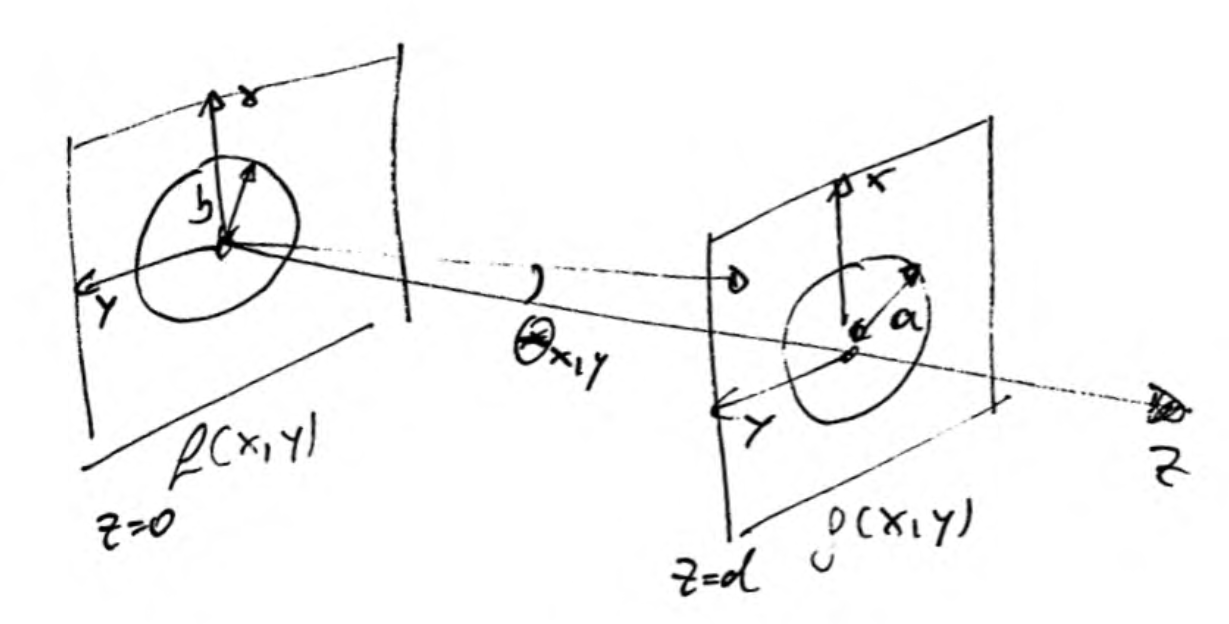
\includegraphics[width=\textwidth]{\currfiledir sketches/fraunhofer.png}
    \caption{Fraunhofer condition}
\end{marginfigure}

The Fourier components $F$ of the field $f$ in the source plane determine the direction of travel of the plane waves, as we have seen above. The problem is that a plane wave is everywhere in space. We need thus to find a condition for 'far enough' so that the individual pieces of the plane wave have separated enough. We do not only employ the paraxial approximation, i.e., that the wave vectors are not too inclined on the optical axis. The key point is that we also require the size of the source plane to be limited. This leads to the two conditions of the Fraunhofer approximation
\begin{equation}
    N_F =  \frac{a^2}{\lambda d} \ll 1 \quad \text{and} \quad
    N_{F}' =  \frac{b^2}{\lambda d} \ll 1 
\end{equation}
where the two $N_F$ are the Fresnel numbers, and $a$,$b$ are the radius of the relevant and allowed regions in the target and source planes, respectively. $d$ is again the distance between the  planes. The Fraunhofer approximation is a more severe restriction than the Fresnel approximation.

We start by writing down the convolution integral of eq. \ref{eq:2_gfh_conv} in the Fresnel approximation
\begin{align}
    g(x,y) = & f(x,y) \otimes h(x,y)_\text{Fresnel} \\
 = & h_0 \iint f(x', y') \,  \exp \left(i k \frac{(x-x')^2 + (y-y')^2 }{2d} \right)  \, dx' dy' \quad .
\end{align}
The term $(x-x')^2$ in the exponent of the exponential function is multiplied out into three terms. 
We keep the mixed terms. Both squared terms can be neglected due to the Fraunhofer approximation. For example  we get 
\begin{equation}
    \exp \left(i \pi  \frac{x'^2 + y'^2 }{ \lambda d} \right) \approx 1
\end{equation}
as  $N_{F}' \ll 1$. The terms without prime vanish due to $N_{F} \ll 1$. So we have
\begin{equation}
    g(x,y)  \approx h_0   
     \iint f(x', y') \,  \exp \left(-i 2 \pi \frac{x x' + y y' }{\lambda d} \right)  \, dx' dy' \quad .
\end{equation}
We now identify  the factor $x / \lambda d$ with the spatial frequency  $\nu_x$ ($y$ similar) and write
\begin{equation}
    g(x,y) \approx h_0
     F \left( \nu_x,\nu_y \right) 
     =  h_0
     F \left( \frac{x}{\lambda d}, \frac{y}{\lambda d} \right) \quad .
\end{equation}

When we place a screen $g$ at a distance fulfilling the Fraunhofer condition after a diffracting obstacle $f$, the interference pattern visible on the screen will be described by the Fourier transform $F$ of $f$. This simplifies a lot the calculation of single slit, double slit and grating, as typically  presented in the  introductory optics lecture.

\begin{questions}
    \item Convince yourself that the textbook solution, for example in Demtröder, can be obtained by a Fourier transform.
    \item Estimate the required distance so that a typical diffraction grating fulfils the Fraunhofer condition.
\end{questions}


\section{Optical Fourier transform by a lens}

The distance $d$ required to stay within the Fraunhofer approximation can be prohibitively large. We will see here that a lens is able to shorten the distance between the grating and the screen and still keep the Fourier relation. This explains why spectrometers are not too long, but contain a lens or curved mirror.

\begin{marginfigure}
    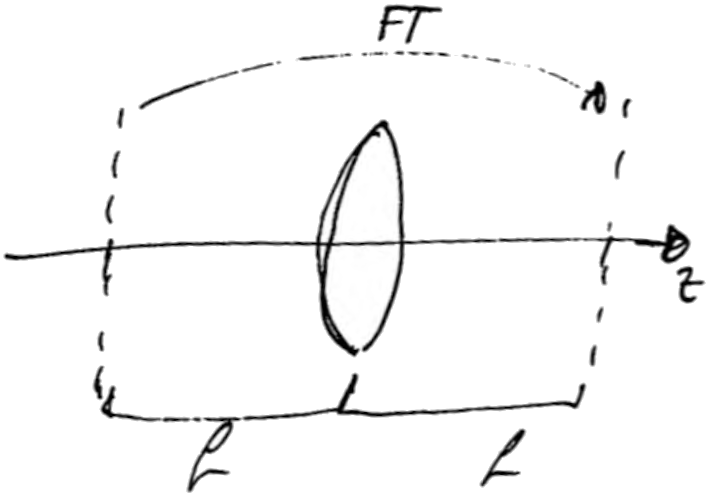
\includegraphics[width=\textwidth]{\currfiledir sketches/lens.png}
    \caption{Optical Fourier transform by a lens}
\end{marginfigure}

From geometrical optics in the paraxial approximation we know already that a lens focuses a beam  (angles $\Theta_x$, $\Theta_y$ to the optical axis) on a point 
\begin{equation}
(x,y) = (f \Theta_x, f \Theta_y)
\end{equation}
in the focal plane, where $f$ describes the focal length of the lens. A lens thus separates plane waves by their propagation direction. As in the beginning of the chapter, we can convert angles into optical frequencies and thus find that the field in the target plane $g$ is proportional the the Fourier amplitude $F$
\begin{equation}
    g(x,y) = \tilde{h} \,   F \left( \nu_x,\nu_y \right) = \tilde{h} \,  F \left( \frac{x}{\lambda d}, \frac{y}{\lambda d} \right) \quad .
\end{equation}
The remaining question is the prefactor $\tilde{h}$. If it would depend of the spatial coordinates $x$ and $y$, this would destroy the Fourier transform. To obtain $\tilde{h}$, we multiply the transfer functions of free space for the distance source plane to lens (length $d$) and lens to target plane (length $f$). And we need to multiply a transfer function for the lens, as the lens has a thickness profile $t(x,y)$ of a material with a certain index of refraction. All together one obtains\sidenote{details in \cite{SalehTeich1991}, chapter 4}
\begin{equation}
    \tilde{h}(x,y) =  \tilde{h}_0 \exp \left( 
-i \pi \frac{(x^2 - y^2)(d-f)}{\lambda^2 f}
    \right) \quad \text{with} \quad  \tilde{h}_0  = \frac{-i}{\lambda f} \, e^{ik (d+f)} \quad .
\end{equation}
This factor becomes spatially constant when the condition $d=f$ is met. A lens thus performs an optical Fourier transform between is two focal planes. In a spectrometer, the grating sits in the front focal plane of the curved mirror (acting as a lens), the detector in its back focal plane.



\section{Spatial filter}


In addition to spectrometers, the spatial filter is another important application of a lens as a Fourier transform device. We consider a so-called 4f-system, see \cite{SalehTeich1991}. All components are separated by one focal length $f$: a source plane $f$, a first lens, a filter plane $p$, a second lens and a target plane $g$. Both lenses are identical. 

\begin{marginfigure}
    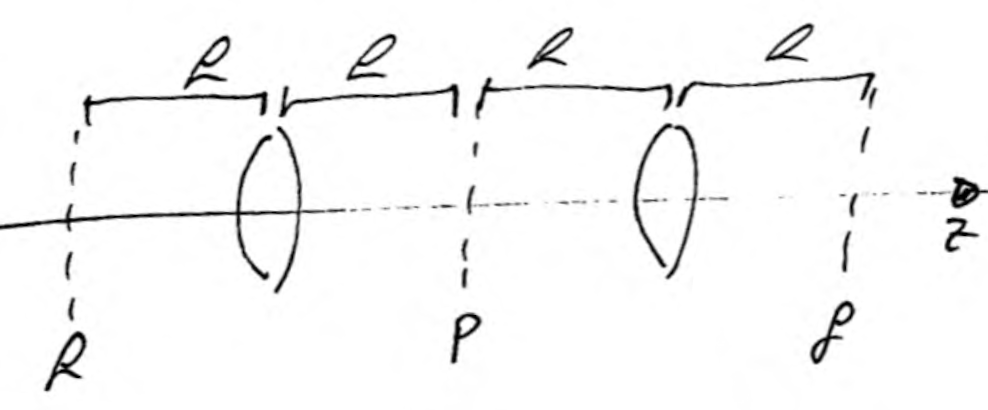
\includegraphics[width=\textwidth]{\currfiledir sketches/spatial_filter.png}
    \caption{A $4f$ system can be used as spatial filter.}
\end{marginfigure}

Let the transfer function $p$ of the filter plane be $p(x,y)=1$ for the beginning. Then the first lens Fourier transforms $f$ into $F$ in the filter plane. The filter does nothing and the second lens transforms back $F$ into $f$, so that we get in the target plane what we started with , i.e., $f=g$. Of course this make the assumption that all plane waves nicely propagate, i.e., the spatial frequencies in $f$ are small enough to cause only propagating plane waves.

The filter plane can be used to modify the Fourier components $F$. At position $x$ in the $p$ plane, only the Fourier component $\nu_x = x / (\lambda f)$ is present. We can put a mask $p(x,y)$, either just absorbing or with a complex transfer function in the filter plane. The overall transfer function of the 4f-system is then
\begin{equation}
    H(\nu_x, \nu_y) = p (\lambda f \nu_x, \lambda f \nu_y) \quad , 
\end{equation}
ignoring an overall phase factor for the propagation. 

An often used transfer function is a circular aperture. It removes all spatial frequencies above a certain threshold. In this way, one can clean up a laser beam, so that is follows the expected Gaussian profile even after transmission though many non-ideal optical elements.

The inverse filter, i.e. a opaque disc, acts as high-pass filter, increasing the edges in an optical image. A vertical slit lets only pass horizontal features in the image.



%--------------------
\printbibliography[segment=\therefsegment,heading=subbibliography]

\renewcommand{\lastmod}{October 27, 2023}
\renewcommand{\chapterauthors}{Markus Lippitz, Christoph Schnupfhagn}

\chapter{Spatial Light Modulator}

\section{Overview}

In optics, we not only Fourier transform between the two focal planes of a lens, but we can also Fourier transform between energy and time. A spatial light modulator (SLM) spatially modulates light (in the image plane of a grating spectrometer) to shape the temporal evolution of ultrafast ( $\approx 10$~fs) laser pulses. We follow the formalism of \cite{Traeger2012}.

\section{Generation and properties of ultrashort laser pulses}

To build a laser we need at least a cavity, an active medium and a pump source. The cavity has longitudinal modes if multiples of the half wavelength fit into the cavity length $l$. For integer $n$ and wavelength $\lambda$ this standing-wave condition reads ${l = n\lambda/2}$. Consequently, the resonances are equidistant in frequency space at $\omega_{n} = n\pi c/l$, where $c$ is the speed of light.  
In general, the electric field $E(x,t)$ results from a superposition of all cavity modes $\omega_{n}$ with individual amplitudes $A(\omega_{n})$ and relative phases $\phi_{n}$
\begin{equation}
	E(x,t) = \Re \left[ \sum_{i} A(\omega_{i}) e^{i (\omega_{i} t - k x + \phi_{i})} \right] \quad .
\end{equation}
The wave vector $k$ is given by the dispersion relation $k=\omega/c$.
The spatial dependence is dropped for simplicity. The electric field in time domain is linked to its counterpart in frequency domain by Fourier transform
\begin{equation}
	E(\omega) = \mathcal{F}[E(t)] = \int_{-\infty}^{\infty} E(t) e^{- i \omega t} dt \quad .
\end{equation}
Since $E(\omega)$ is complex-valued while $E(t)$ is a real function, it follows $E(\omega) = E^{*}(-\omega)$. Therefore, it is sufficient to look only at the positive frequencies $E^{+}(\omega)$ and  one separates them by writing
\begin{equation}
	E(\omega) = E^{+}(\omega) + E^{-}(\omega) \quad ,
\end{equation}
where
\begin{equation}
	E^{+}(\omega) = \left \{ 
	\begin{aligned}
		& E(\omega) &&\text{if } \omega \geq 0 \\
		& 0 && \text{if } \omega < 0
	\end{aligned} \right.
	\qquad \text{and} \qquad
	E^{-}(\omega) = (E^{+}(-\omega))^{*} \quad .
	%\left \{ 
	%\begin{aligned}
%		& 0 &&\text{if } \omega \geq 0 \\
%		& E(\omega) && \text{if } \omega < 0
%	\end{aligned} \right. \quad .
\end{equation}
The Fourier transform of $E^{+}(\omega)$ is then
\begin{equation}
	E^{+}(t) = \frac{1}{2\pi} \int E^{+}(\omega) e^{ i \omega t} d\omega \quad .
\end{equation}
And of course we can decompose the complex $E^{+}(\omega)$  into phase and amplitude
\begin{equation}
	E^{+}(\omega) = | E^{+}(\omega) | \,  e^{- i \phi(\omega)} \quad .
\end{equation}
In order to generate short laser pulses, the phase relation $\phi(\omega)$ between the laser modes needs to be fixed in time. This is called \emph{mode locking}. Additionally, to generate confined pulses in time domain Fourier's theorem requires a broad distribution in the frequency domain, i.e., an active medium with a broad gain spectrum. This is expressed by the product of temporal width $\Delta t$ (full width at half maximum, FWHM) and spectral width $\Delta\nu$ (FWHM), which can not be smaller than a minimum value TBP$_{\text{min}}$
\begin{equation}
	\Delta t \cdot \Delta \nu \geq \text{TBP}_{\text{min}} \quad .
\end{equation}
This minimum \emph{time-bandwidth product} (TBP) depends on the temporal shape of the pulse. In case of a Gaussian shape the value is TBP$_{\text{min}} = 0.441$, i.e., 7 fs pulses centered at 800 nm require a minimum spectral width of approximately 135 nm.

\begin{questions}
	\item Superimpose in increasing number of harmonic functions with equidistant frequencies to synthesis a laser pulse.
	\item Vary the phase relation between these modes to simulate a light field that is not 'mode locked'
\end{questions}

\section{Spectral phase}

The actual pulse duration for a given spectrum strongly depends on the spectral phase $\phi(\omega)$. In general, the first derivative of the phase with respect to frequency is called \emph{group delay} (GD) while the second derivative is called \emph{group delay dispersion} (GDD). Expanding the phase in a Taylor series around the central frequency $\omega_{0}$ yields
\begin{equation}
	\begin{aligned}
	\phi(\omega) = & \phi(\omega_{0}) + \phi'(\omega_{0})(\omega-\omega_{0}) + \frac{1}{2} \phi''(\omega_{0})(\omega-\omega_{0})^{2} \\
	& +  \frac{1}{6} \phi'''(\omega_{0})(\omega-\omega_{0})^{3} + ... \quad ,
	\end{aligned}
\end{equation}
where
\begin{equation}
	\phi^{(n)} = \left. \frac{\partial^{n}\phi}{\partial \omega^{n}} \right\rvert_{\omega=\omega_{0}} \quad .
\end{equation}
The propagation of laser pulses is determined by the optical properties of the materials, in particular the dispersion of the refractive index $n(\omega)$. As the refractive index in general varies with the frequency, the spectral colors gather different phase shifts during propagation. The variations are most pronounced in the vicinity of material resonances, affecting also higher orders in the Taylor expansion of the phase. To illustrate this, the influence of the different orders in the Taylor expansion on the temporal shape of bandwidth-limited 7~fs pulses is shown in Figure \ref{fig:3-pulses}.

\begin{figure}
	\centering
	\includegraphics[width=\textwidth]{\currfiledir pulses_complete.pdf}
\caption{Dependence of the temporal pulse shape on different orders in the Taylor expansion of $\phi(\omega)$. The Gaussian shaped pulses have a bandwidth limit of 7~fs and are centered at 800~nm. }
\label{fig:3-pulses}
\end{figure}



A constant phase term defines the phase difference between the carrier wave and the envelope, known as the carrier-envelope phase (CEP) without altering the pulse shape. Similarly, a linear phase term shifts the pulse in time without any distortions, where the value of $\phi'$ is equivalent to the introduced time offset.

In contrast, applying a quadratic phase term, also called \emph{linear chirp}, stretches the pulse in time. Energy conservation then requires the peak intensity to decrease. Furthermore, the different frequencies do not arrive simultaneously: The red colors arrive before the blue in case of $\phi''>0$, which is typical for most materials. Ultrashort pulses are exceptionally affected by temporal broadening since the large spectral bandwidth allows for large spectral variations of the refractive index. 

The figure shows a pulse broadening from 7~fs to 21~fs (FWHM) at $\phi'' = 50$~fs$^{2}$, corresponding to a transmission through 1.2~mm \ch{SiO_2} glass at 800 nm. This small propagation length already increases the TBP by a factor of 3 from $0.441$ to $1.323$. At the same time the peak intensity is reduced by 67~\%. Other glasses yield even higher GDD values\footcite{Traeger2012}, e.g., $\phi'' \approx 143$~fs$^{2}$ in SF10.

Applying even higher orders in the phase expansion creates increasingly complex pulse shapes; a cubic phase term for instance generates multi-pulse sequences which are asymmetric in time. 

In an experiment, one usually needs the shortest possible laser pulse at the sample. Optical elements between laser and sample can contribute a complex optical phase. It is one task of the spatial light modulator to compensate these phase differences.



\section{Pulse shaping with spatial light modulators}
	
Since both the intensity spectrum and the spectral phase determine the pulse shape in time domain, it is desirable to control both parameter sets in the experiment. This can be achieved with a spatial light modulator which directly addresses the frequency domain in a $4f$ setup as illustrated in Figure \ref{fig:3-4f}: The spectral colors of incident pulses with electric field $E_{\text{in}}( \omega)$ are spatially separated by a diffraction grating. A lens with focal length $f$ focuses each color into its Fourier plane, which is again located in a distance $f$. In this plane a complex transfer function $H(\omega) = A(\omega) \, e^{i \phi(\omega)}$, consisting of amplitude and phase term $A(\omega)$ and $\phi(\omega)$, can be applied. This could, e.g., be realized with a glass plate having a spatially varying thickness to generate a frequency-dependent phase function. An additional metallic coating might, similar to a filter wheel with variable optical density, create the amplitude mask. However, a more sophisticated way to shape pulses is to use liquid crystal masks instead of static masks where each pixel controls a different frequency. After the spectral modifications, the colors are recombined and collimated with an additional lens-grating combination in distance $f$, yielding the output electric field distribution
\begin{equation}
	E_{\text{out}}^{+}(\omega) = H(\omega) \, E_{\text{in}}^{+}(\omega) \quad .
\end{equation}
A multiplication in frequency domain corresponds to a convolution in time domain, therefore
\begin{equation}
	E_{\text{out}}^{+}(t) = \mathcal{F}\left[H(\omega)\right] \otimes E_{\text{in}}^{+}(t) \quad ,
\end{equation}
where $\otimes$ denotes the convolution. 


\begin{figure}
	\centering
	\includegraphics[width=0.7\textwidth]{\currfiledir slm_setup.pdf}
	\caption{Sketch of a $4f$ setup consisting of two gratings and lenses. The incoming electric field $E_{\text{in}}(\omega)$ is manipulated by a transfer function $H(\omega)$ in the Fourier plane of the lens, resulting in an outgoing field $E_{\text{out}}(\omega)$. }
	\label{fig:3-4f}
\end{figure}


\section{Typical masks}

A \emph{linear phase}
\begin{equation}
	\phi(\omega) = \tau (\omega-\omega_{0})
\end{equation}
translates the laser pulse by the $\tau$ in time, without any further spectral modification. The maximum accessible value of $\tau$ depends on the maximum phase change of the SLM. Values around 1~ps are typical, corresponding to 300~\textmu m travel.

A \emph{polynomial phase mask}
\begin{equation}
	\phi(\omega) = \sum_{n} \frac{a_{n}}{n!} (\omega-\omega_{0})^{n}
\end{equation}
will be used frequently in order to compensate the group delay dispersion of optical elements. Its parameters $a_n$ correspond the the Taylor coefficients of the phase dispersion.


The \emph{sinusoidal phase mask}
\begin{equation}
	\phi(\omega) = a  \cos \left[ \tau  (\omega-\omega_{0}) - \Delta\phi \right] \quad .
\end{equation}
generates a  train of a few pulses\footcite{Renard04}, separated by $\tau$ in time. The amplitude of the $n$-th puls is controlled by the modulation amplitude $a$ and is proportional to the Bessel function of first kind $J_n(a)$.

A \emph{V-shaped phase mask} splits the spectrum at $\omega_s$
\begin{equation}
	\phi(\omega) = 
\left\{
\begin{matrix}
	- \tau_{-} (\omega-\omega_s) & \quad \text{for} & \omega < \omega_s \\
	+ \tau_{+} (\omega-\omega_s) & \quad \text{for} & \omega  \ge \omega_s 
\end{matrix}
\right.	
\end{equation}
and separates both spectral components by $\tau_{+} + \tau_{-}$ in time. This is similar to pump-probe spectroscopy, where two laser pulses interact with the sample.

The \emph{sinusoidal amplitude mask}
\begin{equation}
	A(\omega) = \cos \left[ \frac{\tau}{2} (\omega-\omega_{0}) - \Delta\phi \right] \quad .
\end{equation}
creates two identical copies of the pulse separated by a time delay $\tau$. The carrier-envelope phase of both pulses is the same unless $\Delta\phi \neq 0$. This amplitude mask can be used to measure the autocorrelation of a laser pulse. Note that here $A$ changes sign. Depending on the implementation, one might want to leave $A >0$ and include a $\pi$ phase shift.




\section{Realization by liquid crystals}


How could one change   amplitude $A$ and phase $\phi$ of the optical field at each pixel? A variation in phase is obtained from a variation of the index of refraction that is experienced by the light field. The amplitude is modified by rotating the direction of linear polarization of the field, and then letting it pass through a linear polarizer, which removes the unwanted fraction of the amplitude. So we need to briefly look into polarization optics and birefringence to understand the working of the spatial light modulator.


First we need a birefringent material as used in polarization optics, but the amount of birefringence should be controllable from the outside. This we find in liquid crystals.
Uniaxial liquid crystals are anisotropic materials which can be approximated by an ellipsoidal molecular shape. The anisotropic shape results in an index of refraction that depends not only on the polarization direction, but also on the angle $\Theta$ between the wave vector $\bk$ and the symmetry axis of the molecule. The latter is called 'optic axis' in polarization optics, not to be confused\sidenote{in German, \emph{both} is 'optische Achse' !} with the 'optical axis'. 
Light is  decomposed into ordinary and extraordinary rays with refractive indices $n_{\text{o}}$ and $n_{\text{eo}}(\theta)$, respectively. While $n_{\text{o}}$ does not depend on $\Theta$, we have for $n_{\text{eo}}$
\begin{equation}
	\frac{1}{n_{\text{eo}}^{2}(\theta)} = \frac{\cos^{2}\theta}{n_{\text{o}}^{2}} + \frac{\sin^{2}\theta}{n_{\text{eo}}^{2}(90^{\circ})} \quad .
\end{equation}
 
By the manufacturing process of the electrodes a preferential direction, called \emph{director}, is given. Without external electric field, the molecules align in this direction.  Applying an electric field, the molecules orient in this field and turn. The angle $\Theta$ thus changes and so does the index of refraction. The phase difference $\Delta \phi$ between light polarized parallel and perpendicular to the director depends thus on the applied voltage $U$
\begin{equation}
	\Delta\phi(\omega,U) = \frac{\omega d}{c_{0}} \left[ n_{\text{eo}}(\omega,U) - n_{\text{o}}(\omega) \right] \quad .
\end{equation}
The exact relation has no analytical solution and needs to be calibrated.

\begin{figure}
	\centering
	\includegraphics[width=\textwidth]{\currfiledir liquid_crystal_combined_new.pdf}
	\caption{(a) Sketch of a single liquid crystal mask. (b) The liquid crystal molecules (gray) are aligned along the electrode surface (blue) if no voltage is applied. For voltages ${U>0}$ the tilting angle $\theta$ of the molecules changes. (c) In the experiment, two liquid crystal masks are placed between crossed polarizer.}
	\label{fig:3-lq-display}
	\end{figure}

This gives only one degree of freedom. In the devices, two liquid crystal panels (A,B) are put directly after each other, but with directors rotated by 90 degrees. Before and after the SLM two linear and crossed polarizers are placed. The two directors are under $\pm$45 degrees to them.  The transmitted electric field is then
\begin{equation}
	E^{+} = E_{0}^{+} \sin\left(\frac{\Delta\phi_{\text{A}}-\Delta\phi_{\text{B}}}{2}\right) \exp\left[ i \left(\frac{\Delta\phi_{\text{A}}+\Delta\phi_{\text{B}}+\pi}{2}\right) \right].
	\label{eq:3_theory-transmitted-E}
\end{equation}
It is apparent that this setup imposes an amplitude and phase term to the electric field, depending on the sum and difference of $\phi_{\text{A}}$ and $\phi_{\text{B}}$, respectively. Therefore, by varying the voltages $U_{\text{A}}$ and $U_{\text{B}}$ amplitude and phase of the transmitted field can be independently tuned. Since the SLM is positioned in the Fourier plane, this allows to shape the pulses over the complete spectral bandwidth.

  


% Due to the inherent anisotropy liquid crystals show birefringence, i.e., the refractive index of light depends on the polaization direction relative to the long axis of the molecule. This symmetry axis is called 'optic axis', which should not be confused\sidenote{in German, \emph{both} is optische Achse ...} with 'optical axis'. Not only the shape of the mocule, but also the index of refaction is represendted by an ellipsoid (see Fig XXX) When a wave travel in direction $\bk$, we intersect the index ellpsoid with a plane permedicualr to $\bk$ and going through the center of the ellispod. This intersection has the shape of an ellips. The two major axes give the direction and value of the refarctive index seen by the ordinary (o) and extraordinary (eo) polarization. As the ellipsoid is unixaliu $n_o$ is constant, idepebdet of the angle $\Theta$ begweern $\bk$ and the optic axis. For $n_\text{eo}$ we find
% \begin{equation}
% 	\frac{1}{n_{\text{eo}}^{2}(\theta)} = \frac{\cos^{2}\theta}{n_{\text{o}}^{2}} + \frac{\sin^{2}\theta}{n_{\text{eo}}^{2}(90^{\circ})} \quad ,
% \end{equation}

% polarized along the long axis differs from the orthogonal direction. In general, incident light is therefore decomposed into ordinary and extraordinary rays with refractive indices $n_{\text{o}}$ and $n_{\text{eo}}(\theta)$, respectively. The index $n_{\text{eo}}$ depends on the angle $\theta$ between the direction of light propagation and the optical axis which can be easily seen from the two extreme cases: If light is traveling along the optical axis, the transversely polarized light 'sees' the circular cross-section of the molecules and therefore $n_{\text{o}} = n_{\text{eo}}(0^{\circ})$. In contrast, if light travels perpendicular to the optical axis, it 'sees' an ellipsoidal cross section, yielding $n_{\text{o}} \neq n_{\text{eo}}(90^{\circ})$. This effect can be generalized by the index ellipsoid equation\cite{Saleh_Teich}
% \begin{equation}
% 	\frac{1}{n_{\text{eo}}^{2}(\theta)} = \frac{\cos^{2}\theta}{n_{\text{o}}^{2}} + \frac{\sin^{2}\theta}{n_{\text{eo}}^{2}(90^{\circ})} \quad ,
% \end{equation}
% where $n_{\text{o}}$ and $n_{\text{eo}}$ depend on the light frequency. Liquid crystal masks are in particular useful for pulse shaping since the direction of the optical axis is tunable by varying the voltage $U$ between the electrodes. The emerging electric field induces a torque on the molecules which is balanced by the torque that tries to align all molecules in the predefined direction. The functional dependence $\theta(U)$ is not known analytically and therefore has to be measured in the experiment, but qualitatively $\theta$ decreases with increasing voltage. Linearly polarized light will gather a phase difference $\Delta\phi$ between the ordinary and the extraordinary ray, depending on the frequency, the thickness $d$ of the liquid crystal cell, the vacuum speed of light $c_{o}$ and the applied voltage \cite{Jenoptik2015}
% \begin{equation}
% 	\Delta\phi(\omega,U) = \frac{\omega d}{c_{0}} \left[ n_{\text{eo}}(\omega,U) - n_{\text{o}}(\omega) \right] \quad .
% \end{equation}



% A Spatial light modulators needs many pixels that shoudl be controlled indiviually. To zis end a single liquid crystal layer is sandwiched between striped transparent electrodes (ITO, indium tin oxide), where the electrode periodicity defines the pixelation of the mask (see Figure \ref{fig:3-lq-display}\,(a)). Similar to an LCD screen, the volatge acorss each opixel is controlled an by this its birefringence




% \begin{figure}
% \centering
% \includegraphics[width=11.5cm]{\currfiledir liquid_crystal_combined_new.pdf}
% \caption{(a) Sketch of a single liquid crystal mask. (b) The liquid crystal molecules (gray) are aligned along the electrode surface (blue) if no voltage is applied. For voltages ${U>0}$ the tilting angle $\theta$ of the molecules changes. (c) In the experiment, two liquid crystal masks are placed between crossed polarizer.}
% \label{fig:3-lq-display}
% \end{figure}

% \section{Amplitude and phase control}

% In the experiment, two consecutive masks A and B are placed between crossed polarizes. The optical axes of the masks are perpendicular to each other, where the directions of the optical axes are rotated by $+45^{\circ}$ and $-45^{\circ}$, respectively. The first polarizer selects only the vertical polarization of the incident electric field, called $E_{0}^{+}$. Each mask introduces a phase difference $\Delta\phi_{\text{A,B}}$ between the ordinary and the extraordinary ray in the electric field. The transmitted electric field is then
% \begin{equation}
% 	E^{+} = E_{0}^{+} \sin\left(\frac{\Delta\phi_{\text{A}}-\Delta\phi_{\text{B}}}{2}\right) \exp\left[ i \left(\frac{\Delta\phi_{\text{A}}+\Delta\phi_{\text{B}}+\pi}{2}\right) \right].
% 	\label{eq:3_theory-transmitted-E}
% \end{equation}
% It is apparent that this setup imposes an amplitude and phase term to the electric field, depending on the sum and difference of $\phi_{\text{A}}$ and $\phi_{\text{B}}$, respectively. Therefore, by varying the voltages $U_{\text{A}}$ and $U_{\text{B}}$ amplitude and phase of the transmitted field can be independently tuned. Since the SLM is positioned in the Fourier plane, this allows to shape the pulses over the complete spectral bandwidth.


%--------------------
\printbibliography[segment=\therefsegment,heading=subbibliography]

\renewcommand{\chapterauthors}{Markus Lippitz}
\renewcommand{\lastmod}{September 18, 2023}


\chapter{X-Ray Scattering}




\section{Overview}
A classic application of Fourier transforms is X-ray scattering to determine a crystal structure, or similar experiments with electrons or neutrons. We will review the differences between the Bragg and Laue formalisms and then discuss the influence of a basis on the diffraction pattern.

\section{How to measure this?}

\begin{figure}
\inputtikz{\currfiledir debye_scherrer_film}
  \caption{Sketch of the diffraction pattern in a Debye-Scherrer powder diffractometer}.
\end{figure}


In a Debye-Scherrer powder diffractometer, a monochromatic X-ray beam passes through a crystalline powder. The radiation that is diffracted is detected by a film that is placed in a ring around the sample. This is why there are notches in the film at $0^\circ$ and $180^\circ$ to allow the X-ray beam to pass through. Concentric elliptical lines are found, each of which has a constant angle of deflection called $2\theta$.

\begin{marginfigure}
\inputtikz{\currfiledir setup}
  \caption{Sketch of a powder diffractometer according to Debye-Scherrer}.
\end{marginfigure}

This method is simpler than the historically older Laue method, which uses a single homogeneous crystal as the diffractive element. The powder contains all the orientations of the crystal with respect to the incident beam. As we will see below with the Ewald sphere, it is rather unlikely that the combination of wavelength, incident direction and grating will lead to constructive interference. In the Laue method, therefore, the crystal must be appropriately oriented and/or broad spectrum X-rays must be used.

The formalism presented in this chapter is not restricted to the diffraction of X-rays. You can also diffract visible light, electrons or neutrons in a completely analogous way. The relationship between energy per particle and wavelength is different. Short wavelengths can be obtained with massive particles at lower energies.  The choice of beam also determines whether the distribution of electrons (X-rays) or nuclei (neutrons) is studied.

\section{Basic idea of scattering theory}

How does a wave interact with a given arrangement of objects? This question is answered by the scattering theory. In this section, we remain general, specifying neither the type of wave (light, electrons, neutrons), nor the type of objects (gaps, electrons, nuclei). The nomenclature follows \cite{Hunklinger2014}.

A plane, here for simplicity scalar wave $A(t)$ thus
\begin{equation}
 A(t) = A_0 \, e^{- i \, (\omega_0 t - \mathbf{k}_0 \cdot \mathbf{r})}
\end{equation}
is described by the amplitude $A_0$, angular frequency $\omega_0$ and wave vector $\mathbf{k}_0$. This wave falls on the point-like scattering center at the origin of the coordinate system and generates  an outgoing spherical wave of the form
\begin{equation}
 A_Z(t) = \frac{\tilde{A}}{R} \, e^{- i \, (\omega_0 t - k_0 R)}
\end{equation}
where the spherical wave depends only on the distance $R = |\mathbf{R}|$ to the center of the sphere and the magnitude $k_0 = | \mathbf{k}_0| $ of the wave vector. The amplitude $\tilde{A}$ depends on the efficiency of the process.

\begin{marginfigure}
\inputtikz{\currfiledir kugelwelle}
\caption{Sketch scatter at a point}
\end{marginfigure}

An extended sample thus consists of many scattering centers over which one sums the amplitudes. However, one must consider the phase difference of the individual waves when integrating over many scattering centers. For two scattering centers, one at the origin, the other at $\mathbf{r}$, one finds by geometrical considerations the phase difference
%
\begin{marginfigure}
\inputtikz{\currfiledir two-points-interference}
\caption{Sketch to path difference $dx = \delta \phi / | \mathbf{k}|= ( \mathbf{k} - \mathbf{k}_0 ) \cdot \mathbf{r} / |\mathbf{k}| $ at two scattering centers.}
\end{marginfigure}
%
\begin{equation}
\delta \phi = ( \mathbf{k} - \mathbf{k}_0 ) \cdot \mathbf{r} \quad ,
\end{equation}
if $\mathbf{k}$ is the wave vector of the outgoing scattered plane wave.\sidenote{The spherical wave from above can be written as an integral over plane waves in all spatial directions}. So this gives
\begin{equation}
  A_S(t) = \frac{\tilde{A}}{R} \, e^{- i \, (\omega_0 t - k_0 R)} \,
  \sum_j e^{- i \, ( \mathbf{k} - \mathbf{k}_0 ) \cdot \mathbf{r}_j} \quad .
\end{equation}
Here we made the assumption that the size of the sample, i.e., the differences between the $\mathbf{r}_j$ is small compared to the distance $R$ to the screen. Thus, we are interested in the scattered wave only at a distance so large that, regardless of the location of the scattering center, all partial waves with wave vector $\mathbf{k}$ arrive at the same location. In Fourier optics we called this Fraunhofer approximation. Also, as virtually always in scattering theory, we assume that each wave is scattered only once. This is the Born approximation. 

Now we go from single scattering centers at positions $\mathbf{r}_j$ to a \emph{scattering density} $\rho(\mathbf{r})$, i.e., to the number of scattering centers in a volume element $dV$. Thus the sum becomes an integral and we obtain for the scattered wave
\begin{align}
 A_S(t) = & \frac{\tilde{A}}{R} \, e^{- i \, (\omega_0 t - k_0 R)} \,
  \int_{V_\text{Probe}} \, \rho( \mathbf{r}) \, e^{- i \, ( \mathbf{k} - \mathbf{k}_0 ) \cdot \mathbf{r}} \, dV \
  = & \frac{\tilde{A}}{R} \, e^{- i \, (\omega_0 t - k_0 R)} \, \mathcal{A}(\mathbf{K}) 
\end{align}
with the \emph{scattering amplitude} as Fourier-transformed of the scattering density
\begin{equation}
\mathcal{A}(\mathbf{K}) = \int_{V_\text{probe}} \, \rho( \mathbf{r}) \, e^{- i \, ( \mathbf{k} - \mathbf{k}_0 ) \cdot \mathbf{r}} \, dV = \mathcal{FT} \left\{ \rho( \mathbf{r}) \right\} \label{eq:4_scattering_amplitude}
\end{equation}
and the \emph{scattering vector} $\mathbf{K} = \mathbf{k} - \mathbf{k}_0$. Thus, in scattering experiments, one measures the Fourier transform of the scattering density. This is valid for diffraction at double slit as well as for diffraction of X-rays at electron distribution in a crystal. 



\section{The reciprocal lattice}

If the electron density in the crystal already gives the diffraction pattern as scattering amplitude via Fourier transform, then one can also look at the Fourier transform of, for example, the electron density right away.

The scattering density $\rho(\mathbf{r})$, like all properties of a crystal, is lattice-periodic, i.e. 
\begin{equation}
  \rho(\mathbf{r}) = \rho(\mathbf{r} + \mathbf{T}) = \rho(\mathbf{r} + n_1 \mathbf{a}_1 + n_2 \mathbf{a}_2 + n_3 \mathbf{a}_3) 
\end{equation}
with $n_i$ integers and $\mathbf{a}_i$ primitive unit vectors. Thus $\rho(\mathbf{r})$ is representable as a Fourier series
\begin{equation}
  \rho(\mathbf{r}) = \sum_{h,k,l} \, \rho_{hkl} \, e^{i \, \mathbf{G}_{hkl} \cdot \mathbf{r}}
\end{equation}
with $h,k,l$ integers, the Fourier coefficient as integral over the primitive unit cell PUC
\begin{equation}
\rho_{hkl} = \frac{1}{V_\text{PUC}} \, \int_\text{PUC}    \rho(\mathbf{r})\, e^{-i \, \mathbf{G}_{hkl} \cdot \mathbf{r}} \, dV \label{eq:4_rho_hkl}
\end{equation}
and the  \emph{reciprocal lattice vectors}
\begin{equation}
\mathbf{G}_{hkl} = h \mathbf{b}_1 + k \mathbf{b}_2 + l \mathbf{b}_3 \quad .
\end{equation}
The $\mathbf{b}_i$ are the primitive unit vectors of the reciprocal lattice. $\mathbf{G}_{hkl}$ thus describes the set of all lattice points. Each of these lattice points is associated with exactly one Fourier coefficient $\rho_{hkl}$ of the scattering density. 


\section{Bragg Theory of Diffraction}

The scattering amplitude $\mathcal{A}(\mathbf{K})$, i.e. the amplitude of the scattered wave in the direction $\mathbf{K} = \mathbf{k} - \mathbf{k}_0$, is simply the Fourier transform of the scattering density $\rho(\mathbf{r})$ in real space. Bragg theory is another way of finding the conditions for constructive interference and hence peaks in the scattering image. Below we will merge the different ways.

In which direction $\mathbf{K} = \mathbf{k} - \mathbf{k}_0$ do strong peaks occur in scattering experiments with X-rays, electrons, or neutrons? Bragg theory assumes that atoms form planes at distance $d$. The (matter) waves are reflected at these planes. If the phase difference is suitable, then there is constructive interference and thus a peak.


\begin{marginfigure}
\inputtikz{\currfiledir bragg}

\caption{Phase difference in reflection at two planes}.
\end{marginfigure}


From geometrical considerations one finds that constructive interference occurs exactly when the \emph{Bragg condition} is satisfied
\begin{equation}
n \, \lambda = 2 \, d \, \sin \Theta \quad .
\end{equation}
Here $n$ denotes the diffraction order, $\lambda$ the wavelength of the (matter) wave, $d$ the distance of the planes and $\Theta$ the angle between incident ray and lattice plane. Of course, since specular reflection is involved, this is also the angle of the outgoing ray with the plane.\sidenote{but not that to the surface normal} The difference 
$\mathbf{K}$ of the wave vectors is perpendicular to the reflecting lattice planes. For the magnitude we find
\begin{equation}
|\mathbf{K}| = |\mathbf{k} - \mathbf{k}_0| = 2 | \mathbf{k}_0| \, \sin \theta \quad .
\label{eq:4_def_k_sin_theta}
\end{equation}
There are, of course, many ways to find planes in a crystal, and thus many directions that satisfy the Bragg condition, i.e., many scattering peaks.
 
 
\section{Laue theory of diffraction} 
 
The Bragg condition only predicts whether there is a peak in a certain direction, but not its intensity. The Bragg theory uses only the lattice periodicity of the scattering density $\rho( \mathbf{r})$, not its exact form. Both changes with the Laue theory\sidenote{Max von Laue, 1879--1960 }.

The intensity of a scattering peak is proportional to the square of the scattering amplitude. With Eq.~\ref{eq:4_scattering_amplitude} we get
\begin{equation}
I(\mathbf{K}) \propto \left| \mathcal{A}(\mathbf{K}) \right|^2 
= \left| \int_{V_\text{probe}} \, \rho( \mathbf{r}) \, e^{- i \, \mathbf{K} \cdot \mathbf{r}} \, dV \right|^2 \quad .
\end{equation}
We repeat again the steps from the beginning of the chapter and write the scattering density as a Fourier sum with the coefficients $\rho_{hkl}$
\begin{equation}
  \rho(\mathbf{r}) = \sum_{h,k,l} \, \rho_{hkl} \, e^{i \, \mathbf{G}_{hkl} \cdot \mathbf{r}}
\end{equation}
with $h,k,l$ integers, the Fourier coefficients $\rho_{hkl}$ and the reciprocal lattice vectors
\begin{equation}
\mathbf{G}_{hkl} = h \mathbf{b}_1 + k \mathbf{b}_2 + l \mathbf{b}_3 \quad .
\end{equation}
In the following, I sometimes omit the indices at $\mathbf{G}$. Thus we obtain for the scattering intensity 
\begin{equation}
I(\mathbf{K}) \propto \left| \mathcal{A}(\mathbf{K}) \right|^2 
= \left| 
 \sum_{h,k,l} \, \rho_{hkl}
  \int_{V_\text{probe}} e^{ i \, (\mathbf{G}- \mathbf{K} )\cdot \mathbf{r}} \, dV \right|^2 \quad .
\end{equation}
The integrand oscillates rapidly with $\mathbf{r}$ and averages away unless $\mathbf{G} = \mathbf{K}$. In this case, the integral just gives the sample volume $V_\text{sample}$.

Thus we have obtained the Laue scattering condition
\begin{equation}
\mathbf{G} = \mathbf{K} \quad .
\end{equation}
The difference of the wave vectors must correspond to a lattice vector. Or the other way around: during diffraction at the lattice, a lattice vector is added to the incident wave vector.  The scattering intensity in this case is
\begin{equation}
I(\mathbf{K} = \mathbf{G}_{hkl} ) \propto \left| \mathcal{A}(\mathbf{K} = \mathbf{G}_{hkl} ) \right|^2 
= \left| \rho_{hkl} \right|^2 V_\text{probe}^2 \quad . \label{eq:4_laue_peak}
\end{equation}
Thus, a single Fourier coefficient determines the intensity of the peak in the $(hkl)$ direction.


A side note on the shape of the peaks in reciprocal space. The position is determined by $\mathbf{G}$. The width is finite, i.e. not delta-shaped, because the sample is finite in size. This is analogous to the width of the diffraction peaks at an optical line grating, which also drops as $1/N_\text{lines}$. Thus, in three dimensions, the width of the peak is $1/V_\text{sample}$. Since the height of the peak is proportional to $ V_\text{sample}^2$, the integral over a peak is proportional to $V_\text{sample}$. This is very convenient, since the intensity of the effect should go linearly with the  amount of matter, and not quadratically as Eq.~\ref{eq:4_laue_peak} suggests.


\section{Equivalence of the two conditions}

We start from the Laue condition $\mathbf{G} = \mathbf{K}$ and derive the Bragg condition from it:
\begin{equation}
 | \mathbf{K} | = |\mathbf{k} - \mathbf{k}_0| = 2 | \mathbf{k}_0| \, \sin \Theta = \frac{4 \pi}{ \lambda} \, \sin \Theta = | \mathbf{G} | = n \, | \mathbf{G} | \quad .
\end{equation}
The first steps are Eq.~\ref{eq:4_def_k_sin_theta} and pure geometric considerations for reflection, so not yet the Bragg condition. In the last step, we exploited the fact that any integer multiple of a lattice vector is also a lattice vector again.\sidenote{$\mathbf{G}$ is, after all, fully named $\mathbf{G}_{hkl}$, i.e., a set of vectors}

Each lattice vector describes a plane wave and thus a set of planes at a distance of 
\begin{equation}
 d = \frac{2 \pi}{|\mathbf{G} | }  \quad .
\end{equation}
 All together this gives the Bragg condition
 \begin{align}
   \frac{4 \pi}{ \lambda} \, \sin \Theta & = n \frac{2 \pi}{d } \\
   2 d \, \sin \Theta & = n \lambda \quad .
 \end{align}
 

\section{Ewald sphere} 
Only a few orientations of a crystal relative to the incident beam produce any reflections at all. The construction of the Ewald sphere makes it possible to identify these orientations and the reflections that are then visible:
\begin{enumerate} \setlength{\itemsep}{0pt}
\item draw the lattice as a point lattice in reciprocal space

\item to draw the incident beam with the wave vector $\mathbf{k}_0$ so that the arrowhead ends at the lattice point $(000)$. This defines the orientation of the beam relative to the crystal.

\item draw a circle / sphere around the start of $\mathbf{k}_0$ with radius $|\mathbf{k}_0|$. This gives all points that satisfy $|\mathbf{k}| = |\mathbf{k}_0|$.

\item All points of the reciprocal lattice that lie on the circle / sphere satisfy the scattering condition $\mathbf{G} =\mathbf{K} $.
\end{enumerate}

\begin{marginfigure}
\inputtikz{\currfiledir ewald}

\caption{Construction of the Ewald sphere}
\end{marginfigure}


In a finite crystal, the lattice points are not mathematical points, but extended by the Fourier uncertainty between real space and reciprocal space. Similarly, no (matter) wave is exactly delta-shaped in frequency space, because the Fourier uncertainty between time and frequency also comes into play. So for physical systems there exists points that lie on the circle.

But of course there are many Ewald spheres where only the point $(000)$ lies on the sphere. So Laue diffraction does not always occur, or the crystal has to be oriented more precisely. The use of broadband radiation, e.g. Bremsstrahlung, makes this easier, but loses the possibility to measure the lattice constant.


\section{Structure factor}

So far we have considered only the mathematical lattice and its diffraction pattern. Now we also consider the base, so especially if it contains more than one atom. The short version is: The lattice determines in which direction reflections can occur. The base determines the intensity of these reflections, which in particular can be zero. This is due to destructive interference between diffracting atoms in one sublattice and those in the other.

At the same time the 'reciprocal' in the reciprocal space becomes clear here also once more. The mathematical lattice is 'larger' in real space in the sense that it is described by integer factors (i.e. $\ge 1$) in front of the primitive unit vectors. The base is described by factors between zero and one. In reciprocal space, everything goes with the reciprocal. The mathematical lattice is then 'smaller' than the Fourier transform of the basis. In units of the primitive reciprocal vector of the lattice, the basis is now responsible for effects not between zero and one, but for those at integers $\ge 1$, i.e. the modulation of the amplitude of the diffraction peaks.

We start from Eq.~\ref{eq:4_scattering_amplitude} and insert the definition of the Fourier components Eq.~\ref{eq:4_rho_hkl}. Thus we obtain
\begin{equation}
\mathcal{A}(\mathbf{K} = \mathbf{G}_{hkl} ) 
= \rho_{hkl} V_\text{sample}
= N_\text{PUC} \, \int_\text{PUC}    \rho(\mathbf{r})\, e^{-i \, \mathbf{G}_{hkl} \cdot \mathbf{r}} \, dV 
\end{equation}
with the number of primitive unit cells $ N_\text{PUC} = V_\text{probe} / V_\text{PUC}$.
We now divide the integral over the primitive unit cell into a sum over the atoms of the unit cell and an integral over the direct environment of the atoms. In the end, we integrate over the whole unit cell again. The old spatial coordinate $\mathbf{r} = \mathbf{r}' + \mathbf{r}_\alpha$ we write as the sum of the position of the atom $\mathbf{r}_\alpha$ and the local coordinate $\mathbf{r}'$ in its vicinity. Thus we obtain
\begin{equation}
\mathcal{A}(\mathbf{K} = \mathbf{G}_{hkl} ) 
= N_\text{PUC}  \, 
\sum_\alpha e^{-i \, \mathbf{G}_{hkl} \cdot \mathbf{r}_\alpha} \, \int_{V_\alpha}  
 \rho_\alpha(\mathbf{r'})\, e^{-i \, \mathbf{G}_{hkl} \cdot \mathbf{r'}} \, dV' \quad .
\end{equation}
The integral over the scattering density in the vicinity of the atom $\alpha$ is a Fourier transform and atom-specific. Therefore one defines an \emph{atomic scattering factor} (or also \emph{atomic form factor}) $f_\alpha ( \mathbf{G} )$ as a Fourier transform of the atomic scattering density
\begin{equation}
  f_\alpha ( \mathbf{G} ) = \mathcal{FT} (\rho_\alpha(\mathbf{r}))
\end{equation}
and receives
\begin{align}
  \mathcal{A}(\mathbf{K} = \mathbf{G}_{hkl} ) 
  = &
   N_\text{PUC} \, 
  \sum_\alpha f_\alpha ( \mathbf{G}_{hkl} ) \, e^{-i \, \mathbf{G}_{hkl} \cdot \mathbf{r}_\alpha}   \quad .
  \end{align}

The coordinates $\mathbf{r}_\alpha$ of the atomic positions depend only on the crystal structure, i.e., the Bravais lattice. We write the position in the primitive unit vectors $\mathbf{a}_i$ as
\begin{equation}
\mathbf{r}_\alpha = u_\alpha \, \mathbf{a}_1 + v_\alpha \, \mathbf{a}_2 + w_\alpha \, \mathbf{a}_3
\end{equation}
with $0 \le u,v,w \le 1$. Together with the definition of $ \mathbf{G}$ we then get 
\begin{align}
\mathcal{A}(\mathbf{K} = \mathbf{G}_{hkl} ) 
 = &
  N_\text{PUC}  \, 
\sum_\alpha f_\alpha ( \mathbf{G}_{hkl} ) \, e^{-2 \pi \, i \, ( h u_\alpha + k v_\alpha + l w_\alpha ) } \\
 = &
 N_\text{PUC} \, \mathcal{S}_{hkl} = \rho_{hkl} \, V_\text{probe} 
\end{align}
with the \emph{structure factor} $\mathcal{S}_{hkl} $
\begin{equation}
  \mathcal{S}_{hkl} = \rho_{hkl} \, V_\text{PUC} = \sum_\alpha f_\alpha ( \mathbf{G}_{hkl} ) \, e^{-2 \pi \, i \, ( h u_\alpha + k v_\alpha + l w_\alpha ) }  \quad .
\end{equation}


\section{Example: \ch{CsCl}}

Caesium chloride (\ch{CsCl}) forms a cubic-primitive lattice with a diatomic base, for example with the \ch{Cs} atom at the origin and the \ch{Cl} atom at the center of the space diagonal. Thus the structure factor is 
\begin{equation}
\mathcal{S}_{hkl} = f_\text{\ch{Cs}} \, e^{-2 \pi \, i \, \mathbf{G} \cdot \mathbf{0}} + f_\text{\ch{Cl}} \, e^{- 2 \pi \, i \, \frac{1}{2}(h + k + l) }   \quad .
\end{equation}
The first exponential function is always $1$, the second is $+1$ if the sum $h + k + l$ is even, and $-1$ otherwise. This results in
\begin{equation}
  \mathcal{S}_{hkl} = \left\{
  \begin{array}{@{}ll@{}}
    f_\text{\ch{Cs}}  + f_\text{\ch{Cl}}  &\text{falls}\ h+k+l \ \text{straight} \\
     f_\text{\ch{Cs}}  - f_\text{\ch{Cl}} & \text{falls}\ h+k+l \ \text{odd} \\
  \end{array}\right.  \quad .
\end{equation} 
In X-ray scattering $f_\text{\ch{Cs}}  \approx f_\text{\ch{Cl}}$, so only every second reflection can be seen. In neutron scattering, on the other hand, the atomic structure factors are clearly different and all peaks can be seen.



\section{Example: bcc monatomic and sc diatomic}

A cubic space-centred lattice can be seen as a cubic primitive lattice with a diatomic base. Both describe the same position of the atoms in space. However, they are different mathematical lattices and therefore different $\mathbf{G}_{hkl}$. This apparently results in different peaks in the diffraction pattern, which of course should not be the case.

The resolution is again found in the structure factor. The base needed to turn a cubic primitive into a cubic space-centred lattice is again half the space diagonal, as in the last section. However, unlike in the last section, both positions are now occupied by the same atoms. So all the peaks at odd $ h+k+l $ disappear. These are just the ones that make the difference between $\mathbf{G}_{bcc} $ and $\mathbf{G}_{sc} $. There is a similar condition for the face-centred cubic lattice.


\begin{figure}
\inputtikz{\currfiledir strukturfaktor}
  \caption{If peaks are indexed according to the conventional unit cell, then some are not visible in the centered lattices. }
\end{figure}


\section{Evaluation of powder diffractometry}

The experiment gives the position of the peaks as a function of the double scattering angle $2\Theta$ with known wavelength $\lambda$ of the radiation. From this one would like to determine the possible values of the length of the lattice vector $|\mathbf{G}|$ and thus make a statement about the Bravais lattice, the basis and the lattice constant. In general this is not trivial. In simple cases, like the example at the beginning of the chapter, one can proceed as follows:

We consider the reciprocal distance of the lattice planes
\begin{equation}
\frac{1}{d} = \frac{|\mathbf{G}|}{2 \pi} = \frac{2 \sin \Theta}{ \lambda}  \quad .
\end{equation}
In cubic lattices this is
\begin{equation}
 \sqrt{h^2 + k^2 + l^2} = \frac{2 a \, \sin \Theta}{ \lambda}
\end{equation}
with the lattice constant $a$ of the conventional unit cell in real space, thus 
\begin{equation}
 h^2 + k^2 + l^2 = \left(\frac{2 a }{ \lambda} \right)^2 \, \sin^2 \Theta \quad .
\end{equation}
So one tries to describe the position of all peaks by a single choice of $a/\lambda$ and a set of integers $(hkl)$ each. Thus one obtains the lattice constant $a$ and from the presence or absence of the peaks the structure factor and thus the lattice.



%-------------------

\printbibliography[segment=\therefsegment,heading=subbibliography]



\part{Concept: Hybridization}

\renewcommand{\chapterauthors}{Markus Lippitz}
\renewcommand{\lastmod}{November 8, 2023}


\chapter{Hybridization in classical systems}


\section{Overview}


'Hybridization' is, according to the Cambridge dictionary, 'the process of producing a plant or animal from two different types of plant or animal'. In chemistry, 'orbital hybridization' plays an important role in describing hydrocarbons, for example. Here we want to broaden the view and describe various coupling phenomena from the point of view of hybridization. When two systems couple, they lose their original individual properties, and combined properties emerge. In this chapter we discuss systems of classical physics without quantum mechanics, namely classical mechanical pendulums, phonons in crystals, and Rayleigh scattering of assemblies of nanoparticles.


\section{Coupled Pendulum}

A mathematical pendulum of point mass $m$ and rod length $L$ is governed by the differential equation of its angular displacement $\phi$ in the approximation of small angles $|\phi| \ll 1$
\begin{equation}
 \ddot{\phi} + \frac{g}{L} \, \phi = 0 \quad \text{with} \quad \omega^2 = \frac{g}{L}  \quad , 
\end{equation}
where $g$ is the acceleration due to gravity and $\omega$ its angular eigen-frequency. When two of such pendulums are coupled by a spring between the two masses, we get a coupled system of differential equations
\begin{eqnarray}
 \ddot{\phi_1} + \frac{g}{L_1} \, \phi_1 + \frac{k}{m_1} \, \left( \phi_1 - \phi_2 \right) & = & 0 \\
 \ddot{\phi_2} + \frac{g}{L_2} \, \phi_2 - \frac{k}{m_2} \, \left( \phi_1 - \phi_2 \right) & = & 0 
\end{eqnarray}
with the spring constant $k$.  For the moment, we assume that the pendulums are identical, i.e., $L = L_1 = L_2$ and $m = m_1 =m_2$. The eigen-frequencies are then
\begin{equation}
 \omega_{+}^2 = \frac{g}{L} \quad \text{and} \quad 
  \omega_{-}^2 = \frac{g}{L} + 2 \frac{k}{m} \quad ,
\end{equation}
where in the mode with frequency $\omega_{+}$ both masses move to the same direction, in the $\omega_{-}$ in opposite directions. Only in the latter case the coupling spring comes into play.

To investigate the general case, we assume harmonic oscillations, i.e. $\phi(t) = \phi_0 \, \exp (i \omega t)$ and write the differential equation as matrix
\begin{equation} \boldsymbol{M \, \phi} = 
\begin{pmatrix}
  \frac{g}{L_1} + \frac{k}{m_1}& - \frac{k}{m_1}\\
 - \frac{k}{m_2} & \frac{g}{L_2} + \frac{k}{m_2}
\end{pmatrix}  \boldsymbol{\phi} =  \omega^2 \, \boldsymbol{\phi}
\quad .
\end{equation}
We thus search eigen-values and eigen-vectors of $\boldsymbol{M}$. Assuming individual lengths, but identical masses, we get
\begin{equation}
 \omega_{\pm}^2 = \left( \frac{\omega_1^2 + \omega_2^2}{2} + \frac{k}{m} \right)
  \pm \sqrt{ \left( \frac{\omega_1^2 - \omega_2^2}{2} \right)^2 + \left( \frac{k}{m} \right)^2 } \quad .
\end{equation}
For identical lengths, i.e., identical eigen-frequencies $\omega_1 = \omega_2$, this recovers the results from above.


We see here already the common theme of hybridization: two systems couple. Depending on the ratio of coupling constant (here $k/m$) and energy difference (here $\omega_1^2 - \omega_2^2$), the new eigen-frequencies (or eigen-energies) are closer to the original ones, or split around some kind of average value.


\section{Two coupled oscillators}

Lets do the same with two springs of spring constant $K$. Each spring connects a mass $m_{1,2}$ to the wall, and the masses are connect by a third (coupling) spring of constant $\kappa$. The differential equation in matrix form for harmonic motion along $x$ reads 
\begin{equation} \boldsymbol{M \, x} = 
  \begin{pmatrix}
     \frac{K + \kappa}{m_1} & - \frac{\kappa}{m_1}\\
  -  \frac{\kappa}{m_2} &  \frac{K + \kappa}{m_2}
  \end{pmatrix}  \boldsymbol{x} =  \omega^2 \, \boldsymbol{x}
  \quad .
  \end{equation}
The solutions look very similar to above. For equal masses we get
\begin{equation}
  \omega_{+}^2 = \frac{K}{m} \quad \text{and} \quad 
   \omega_{-}^2 = \frac{K + 2 \kappa}{m}  \quad .
 \end{equation}




 \section{Normal modes}
 
 How does one handle a system of $N$ masses, all connected by more or less harmonic potentials? This is a problem of classical mechanics and leads to the normal modes.\sidenote{see for example chapter 6.3 in \cite{Demtröder_molekuelphysik}}
 
 We use mass-weighted generalized coordinates $q_i = \sqrt{m_i}  \Delta \tilde{q}_i$, where the index $i$ runs over all atoms and all spatial directions, i.e., from $1$ to $3N$. $m_i$ is the mass of the associated atom and $\Delta \tilde{q}_i$ is the deviation from the equilibrium position. Thus, the kinetic energy $T$  is
 \begin{equation}
    T = \frac{1}{2} \sum_{i=1}^{3N} \dot{q}_i^2 \quad .
 \end{equation}
 For the potential we use a Taylor expansion in $q_i$. We set the zero  of the energy scale to the minimum of the potential. Thus the first two terms of the Taylor series disappear and we keep only the next one:
 \begin{equation}
  V \approx \frac{1}{2} \sum_{i,k = 1}^{3N} \frac{\partial V}{\partial q_i \partial q_k} \, q_i \, q_k =. 
   \frac{1}{2} \sum_{i,k = 1}^{3N} b_{ik} \, q_i \, q_k \quad .
 \end{equation}
 Thus we can write the Lagrangian function $L = T - V$ and obtain in this formalism the equations of motion
 \begin{equation}
     \ddot{q}_i + \sum_{k = 1}^{3N} b_{ik} \, q_k = 0 \quad \text{for} \quad i = 1 \dots 3N
 \end{equation}
 or as a matrix with $\tilde{\mathbf{B}} = (b_{ik})$ and $\mathbf{q} = (q_i)$
 \begin{equation}
    \ddot{\mathbf{q}} + \tilde{\mathbf{B}}  \cdot \mathbf{q} = 0 \quad .
 \end{equation}
 This is a system of $3N$ coupled differential equations. To decouple them we diagonalize 
 $\tilde{\mathbf{B}} $, and find $3N$ eigenvectors $\mathbf{q}_n^0$ and (potentially degenerate) eigenvalues $\lambda_n$ so that
 \begin{equation}
       \tilde{\mathbf{B}} \cdot \mathbf{q}_n^0 = \lambda_n \mathbf{q}_n^0 \quad \text{and thus} \quad
        \mathbf{q}_n(t) = \mathbf{q}_n^0 \, e^{i \, t \, \sqrt{\lambda_n}} \quad .
 \end{equation}
 The eigenvectors $\mathbf{q}_n^0$ are called \emph{normal modes}. Thus, they describe the simultaneous motion of all nuclei in all spatial directions at normal mode $n$ with frequency\sidenote{some $\lambda_n$ must be zero, since there can be only $3N - 5$ (or 6) normal modes} $\omega_n = \sqrt{\lambda_n}$. Since the $b_{ik}$ are real-valued, in the normal mode all atoms oscillate in phase, thus making the zero crossing simultaneously, and of course at the same frequency. In the basis of normal modes the potential simplifies: it has only quadratic forms of the kind $\frac{1}{2} k q_i^2$ but no bi-linear ones of the kind $\frac{1}{2} k q_i q_k$, otherwise $\tilde{\mathbf{B}} $ would not be diagonalized.
 

 \section{Chain of coupled masses}

As an example, lets look at the classical chain of coupled masses. We assume all $N$ masses and springs to be equal and take only a movement along the chain into account. The potential then reads
\begin{equation}
    U = \frac{1}{2} \kappa \sum_{n=1}^{N-1} ( \tilde{q}_n - \tilde{q}_{n+1} )^2
\end{equation}
or
\begin{equation}
U = \frac{1}{2} \frac{\kappa}{m} \sum_{n=1}^{N-1}  ( q_n - q_{n+1} )^2 \quad .
\end{equation}
When multiplied out, we get the squared terms $q_n^2$ twice, except for the first and last mass in the chain. And we get terms of neighboring masses $- 2 q_n q_{n+1}$. 
By distribution the cross-terms to the sub- and super-diagonals we get the matrix $B$ as 
\begin{equation}
B =\frac{\kappa}{m} \begin{pmatrix}
 1 & -1 & 0 &  0 & \cdots & 0 \\
-1 & 2 & -1 &  0 & \cdots & 0 \\
0  & -1 & 2 &  -1 & \cdots & 0 \\
0 & 0  & -1 & 2 &   \cdots & 0 \\
\vdots  & & &  &  & \vdots \\
0 &   & \cdots    &    & -1 & 1 \\
\end{pmatrix} \quad .
\end{equation}
We determine the eigenvalues $\lambda_n$ and from them the eigen-frequencies $\omega_n = \sqrt{\lambda_n}$. We find that
\begin{equation}
  \omega_n^2 = \frac{2 \kappa}{m} \left[ 1 - \cos \left(\frac{n-1}{N} \pi \right) \right] 
  \label{eq:5_omega_diag}
\end{equation}
and the eigenvectors describe oscillatory patterns.


What happened here? We coupled oscillators, and the new hybridized system has new eigenfrequencies. If we use many oscillators, we get a continuous band of eigenfrequencies that spans symmetrically around $\omega = \sqrt{2 \kappa / m}$, which is what we would get if a single mass were attached to a wall by two springs.


\section{Analytic approach}

Matrix diagonalization is fine, but tedious for large matrices. Even the derivation of eq.~\ref{eq:5_omega_diag} is beyond my capabilities. I only knew the end of this section. So let us take a different approach.

We now \emph{assume} that the deviation of the masses from their rest position follows a harmonic pattern, which we describe by a wave vector $k = 2 \pi / \lambda$. This way we know what all the masses are doing and we can use an analytical approach.
Let $u_s$ be the deviation of the mass $s$ from its equilibrium position. The force on the mass $s$ is then
\begin{equation}
  F_s = \sum_p \, \kappa_p \left( u_{s+p} - u_s \right)
\end{equation}
with the spring constant $\kappa_p$, which describes how the mass under consideration is  linked to another mass  $p$ lattice sites away. Thus, only the relative displacement of the masses with respect to each other enters. The equation of motion thus becomes
\begin{equation}
    m \frac{d^2 \, u_s}{dt^2} = \sum_p \, \kappa_p \left( u_{s+p} - u_s \right)
\end{equation}
where we have used that all masses are equal. With the ansatz of a plane wave the deviation of the mass with the index $s+p$ becomes
\begin{equation}
    u_{s+p} = U_0 \, e^{-i ( \omega t - k \, a \, (s+p) )}
\end{equation}
with the length $k$ of the wave vector in reciprocal space and the distance $a$ of the lattice points in real space. The term $a (s+p)$ thus describes the equilibrium position of the mass under consideration in real space. If we insert this ansatz into the equation of motion we get
\begin{equation}
- \omega^2 \, m = \sum_p \, \kappa_p \left( e^{i k \, a \, p} - 1 \right) \quad .
\end{equation}
Since all masses are identical, $\kappa_p = \kappa_{-p}$ is reasonable and therefore
\begin{equation}
    \omega^2 = \frac{2}{m} \, \sum_{p=1}^\infty \, \kappa_p \left( 1 - \cos ( k \, a \, p ) \right) \quad .
\end{equation}
Such a relation between frequency $\omega$ and wave vector $k$ is called  \emph{dispersion relation}. It is equivalent to a relation between energy and momentum.

Now we make the additional assumption that only nearest neighbors interact with each other, as in the last section. Thus only $\kappa_{\pm 1} = \kappa $ are different from zero and the sum is omitted. We now also take the root and get
\begin{equation}
\omega = \sqrt{\frac{4 \, \kappa}{m}} \left| \sin \left(\frac{1}{2} \, k \, a \right) \right|  \quad .
\end{equation}

\begin{marginfigure}

\inputtikz{\currfiledir kette_1atom}
\caption{Dispersion relation of a chain of identical masses and springs.}
\end{marginfigure}




\section{Three dimensions}

In three dimensions, we do the same, just keeping track of all neighbors becomes a bit more demanding. Lets discuss the example of 
copper. It has  a face-centered cubic (fcc) crystal structure with a monatomic basis. The reciprocal lattice is thus  body-centered cubic (bcc). The lattice constant is 3.6~\AA.

Our ansatz for the deviation $\mathbf{u}$ from the equilibrium position now contains vectors, $\mathbf{u}_0$ for the amplitude and direction, and $\mathbf{k}$ for the wave vector:
\begin{equation}
  \mathbf{u} = \mathbf{u}_0 \, e^{i ( \mathbf{k} \mathbf{r} - \omega t)} \quad .
\end{equation}
We take only displacements of the masses in the direction $\mathbf{\hat{n}}_i$ of the spring into account and sum over all $i=1 \dots 12$ nearest neighbors. In an fcc-lattice, the neighbors are along the diagonal of each cartesian plane. The sum reads
\begin{equation}
m \frac{d^2 \mathbf{u}}{dt^2} = \sum \kappa_{i} \, [ (\mathbf{u}(\mathbf{r}_i) - \mathbf{u}(0) ) \cdot \mathbf{\hat{n}}_i ]\,  \mathbf{\hat{n}}_i  \quad .
\end{equation}
We insert our ansatz for  $\mathbf{u}$ and get
\begin{equation}
  - \omega^2 m \, \mathbf{u}_0 
 = \sum \kappa_{i} \,  ( e^{i \mathbf{k} \mathbf{r}_i } - 1) [\mathbf{u}_0 \cdot \mathbf{\hat{n}}_i ]\,  \mathbf{\hat{n}}_i \quad .
\end{equation}

This is again an eigen-value equation
\begin{equation}
\mathbf{A} \mathbf{u}_0 = - \omega^2 m \mathbf{u}_0
\end{equation}
with 
\begin{equation}
\mathbf{A}_{uv} = \sum C_{i} \,  ( e^{i \mathbf{k} \mathbf{r}_i } - 1)  \, \mathbf{\hat{n}}_{i, u} \, \mathbf{\hat{n}}_{i, v}
\end{equation}
where $\mathbf{\hat{n}}_{i, v}$ is the $v$-th cartesian component of the normal vector in direction of atom $i$.

\begin{marginfigure}
\inputtikz{\currfiledir fcc-3d_2x}
\caption{Points of high symmetry in the Brillouin zone are marked by large letters. the $\Gamma$ point is the center of the BZ, so $k=0$. The path $\Gamma$--X--K--$\Gamma$--L takes advantage of the symmetry of the Brillouin zone. \label{fig:5_phonon_path} }
\end{marginfigure}

For each value of $\mathbf{k}$, we construct the $3 \times 3$ matrix $\mathbf{A}$ and calculate its eigen-values. We thus obtain a function $\omega(\mathbf{k})$ that has at each point three solutions that are  potentially degenerate (see also Pluto script\pluto{phonon_spring_3d}). This is the dispersion relation. This simple model fits rather nicely the measured data (Fig.\ref{fig:5_phonon_copper}). The entire figure represents the frequency of phonons along a path in reciprocal space shown in Figure \ref{fig:5_phonon_path}. One can take advantage of the fact that reciprocal lattice vectors $\mathbf{G}$ can be added without changing anything. There are only acoustic branches because there is only one atom in the base. The transverse modes are doubly degenerate along the highly symmetric directions. In the [110] direction, the degeneracy is removed.
 

\begin{figure}
\inputtikz{\currfiledir fig_copper_all_model}
\caption{Phonon dispersion in copper (data from \cite{Svensson_cu}) compared to the spring model. The only scaling parameter is the maximum frequency. \label{fig:5_phonon_copper}}
\end{figure}



\section{Rayleigh scattering of small spheres}


And now to something completely different. As oscillators, we use now the collective oscillation of conduction electrons in small metal spheres. These oscillators couple with each other, as each oscillating sphere radiates an electromagnetic wave that interacts with the electrons of the other spheres. We will again find hybridized states with new eigen-frequencies, now in the visible spectral range.

A sphere of radius $R$ and dielectric constant $\epsilon_{in}$ is embedded in a medium of dielectric constant $\epsilon_{out}$. We assume that the radius $R$ is much smaller than the wavelength $\lambda$ of the electromagnetic light field. This means that the phase is constant across the sphere and that we can employ the quasi-static approximation. One solves the Laplace equation taking  boundary conditions and symmetry into account.\footcite{Jackson-ED}\footcite[excercise 2.4.2]{Nolting-ED}\footcite[chapter 5.2]{BH-book}
The sphere responds to the light field with a polarization of
\begin{equation}
 \mathbf{p}(t) = \epsilon_0 \,  \epsilon_{out} \, \alpha \, \mathbf{E}(t)
\end{equation}
with the polarizability
\begin{equation}
 \alpha = 4 \pi  \; R^3 \; \frac{\epsilon_{in} - \epsilon_{out}}{\epsilon_{in} + 2 \epsilon_{out}} \quad .
\end{equation}
We find a resonance when $\epsilon_{in}(\omega) + 2 \epsilon_{out}(\omega) = 0$, which requires one dielectric function to be negative, as it is the case in metals. Small metal particles show thus exceptional strong interaction with light in a certain spectral range. This is the particle plasmon resonance.

As the electric field oscillates $E(t) = E_0 \, e^{-i \omega t}$, also the polarization $p$ oscillates and radiates a secondary, scattered electromagnetic field 
\begin{equation}
  \mathbf{E}_S = \frac{ e^{i \, k  r} }{4\pi\epsilon_0 \, \epsilon_{out}}  \frac{1}{r^3}\left\{
      (k r )^2 \left( \hat{\mathbf{r}} \times \mathbf{p} \right) \times \hat{\mathbf{r}} +
      \left( 1 -  i k r \right)
        \left( 3\hat{\mathbf{r}} \left[\hat{\mathbf{r}} \cdot \mathbf{p}\right] - \mathbf{p} \right)
    \right\} \quad ,
     \label{eq:5_hybrid_Escat}
\end{equation}
where $k = 2 \pi / \lambda$ is the length of the wave vector in the medium. In a driven oscillator, we need a 90 degree phase difference between driving force and oscillator to transfer energy. The power that is absorbed by the dipole\footcite[Chapter 8]{Novotny-Hecht2012} is thus
\begin{equation}
 P_{abs} = \frac{\omega}{c} \, \Im \left( \mathbf{p} \, \mathbf{E}^\star \right)  \quad ,
\end{equation}
so that we get the absorption cross section
\begin{equation}
 \sigma_{abs} = k \, \Im ( \alpha ) =  4 \pi \, k \; R^3 \; \Im \left( \frac{\epsilon_{in} - \epsilon_{out}}{\epsilon_{in} + 2 \epsilon_{out}} \right) \quad .
 \label{eq:5_hybrid_sigma_abs}
\end{equation}
%We are in the Rayleigh  limit of a very small particle so that we can neglect the scattered power. 


We  assume that the surrounding  medium  is a transparent dielectric, i.e., 
$\epsilon_{out}$ is real-valued. The material of the nanosphere should be described by the Drude model of metals. This is often the case when one is far enough away from inter-band transitions that lead to the color of metals, i.e., when one is far enough in the infrared. The dielectric function then reads
\begin{equation}
 \epsilon_{in} (\omega) = \epsilon_{\infty} - \frac{\omega_P^2}{ \omega \left(\omega \;
+ \; i\, \gamma \right) } \quad , \label{eq:5_hybrid_drude}
\end{equation}
where $\epsilon_{\infty} $ is the  high-frequency limit,  $\gamma = 1 / \tau_\text{coll} $ the damping parameter of the plasma oscillation, and $\omega_P$ the plasma frequency 
\begin{equation}
\omega_P = \sqrt{\frac{n \, e^2}{m^\star \epsilon_0}} \quad.
\end{equation}
The plasma frequency depends on the effective electron mass $m^\star$ and number density $n$.

The polarizability $\alpha$ has a resonance when its denominator equals zero, i.e., at $\epsilon_{in} (\omega_{res}) = -2 \epsilon_{out}$. For a Drude metal with low damping this happens at
\begin{equation}
\omega_{res} = \frac{\omega_P}{\sqrt{2 \epsilon_{out} + \epsilon_\infty}} \quad .
\end{equation}
The resonance wavelength in the absorption spectrum thus depends on 
the plasma frequency of the metal and  the dielectric function of the environment. 




 %----------
\section{Plasmon hybridization}

\begin{marginfigure}
\inputtikz{\currfiledir sketch}
\caption{Sketch of the light field shining on two small particles}
\end{marginfigure}


Now we hybridize two particle plasmons. We investigate the optical properties of two small Rayleigh particles which are brought close to each other.  The optical response of each particle is described by  a dipole $ \mathbf{p}_i(t)$, where $i = 1,2$.
 Each dipole experiences the incident field
$\mathbf{E}^{\text{inc}}(\mathbf{r}_i)$ and the field scattered from the other dipole.
The sum of these two fields multiplied by the dipole's polarizability $\alpha_i$
has to give in a self-consistent way the dipole moment (see, for example, \cite{Myroshnychenko08})
%
\begin{align} \label{eq:5_hbyrid_equationsystem}
     \mathbf{p}_1 = &  \epsilon_0 \,  \epsilon_{out} \,  \alpha_1 \left[ \mathbf{E}^{\text{inc}} (\mathbf{r}_1) +
\mathbf{E}^{\text{scat}}_2(\mathbf{r}_1) \right] \\
  \mathbf{p}_2 = &  \epsilon_0 \,  \epsilon_{out} \,  \alpha_2 \left[ \mathbf{E}^{\text{inc}} (\mathbf{r}_2) +
\mathbf{E}^{\text{scat}}_1(\mathbf{r}_2) \right]  \quad . \nonumber
\end{align}
%
The scattered electrical near-field $ \mathbf{E}^{\text{scat}}$ of the dipole $i$ at position of the dipole $j$ is given by eq.   \ref{eq:5_hybrid_Escat} above. As we aim  for a large influence of this scattered field, we will need short distances between the dipoles and thus can focus on the near-field contribution of the scattered field
\begin{equation}
  \mathbf{E}^{\text{scat, nf}}_i(\mathbf{r}_j) = \frac{ 1 }{4\pi\epsilon_0 \, \epsilon_{out}}  \frac{1}{d^3}
        \left( 3\hat{\mathbf{r}}_{ij} \left[\hat{\mathbf{r}}_{ij} \cdot \mathbf{p}_i \right] - \mathbf{p}_i \right)
  \quad ,
\end{equation}
where $\hat{\mathbf{r}}_{ij}   = \mathbf{r} _j - \mathbf{r} _i$ is a vector of length one pointing from the dipole to the point where
the field is evaluated, and $d$ is the distance between the particles.


For simplicity, we assume that both particles have the same dielectric function and are of course embedded in the same medium. 
We  can chose the polarization direction of the incoming electric field  $\mathbf{E}^{\text{inc}}$. Things become simple when we chose it to be either parallel or perpendicular to the connecting axis of the particles. In both cases, the scattered near-field at particle $j$ has the direction of the dipole $i$, which is not the case for other polarization directions. This allows us to use scalar dipole amplitudes $p_i$ and a simplified scattered field amplitude
\begin{equation}
  {E}^{\text{scat, nf}}_i(\mathbf{r}_j) = \frac{ 1 }{4\pi\epsilon_0 \, \epsilon_{out}}  \frac{v}{d^3} \, p_i 
  \quad ,
\end{equation}
where the factor $v$ is $-1$ for perpendicular and $+2$ for parallel polarization.

We solve the equation system for $p_{1,2}$, which we write as effective polarizabilities $\alpha^\text{eff}_{1,2}$
\begin{equation}
 \alpha^\text{eff}_1 = \frac{p_1}{\epsilon_0 \epsilon_{out} \, E^\text{inc}} =  \frac{\alpha_1 - v \, \frac{\alpha_1 \, \alpha_2}{4 \pi d^3}}
 {1- v^2 \, \frac{\alpha_1 \, \alpha_2 }{16 \pi^2 d^6}} 
\end{equation}
and vice versa.
The total polarizability\sidenote{see \cite{Aizpurua_in_Enoch12},  Eq. 5.14}  is then the sum of $\alpha^\text{eff}_{1}$ and $\alpha^\text{eff}_{2}$
\begin{equation}
 \alpha^\text{eff} = \frac{\alpha_1  + \alpha_2 - v \, \frac{\alpha_1 \, \alpha_2}{2 \pi d^3}}
 {1- v^2 \, \frac{\alpha_1 \, \alpha_2 }{16 \pi^2 d^6}} \quad .
 \label{eq:5_hybrid_alpha_eff}
\end{equation}
We are interested in resonance frequencies of $\alpha^\text{eff} $. As both particles are of the same material, the individual polarizability $\alpha_i$ only differ in amplitude due to the factor $R_i^3$. The spectral shape is the same. The effective polarizability comes to resonance when the denominator vanishes, i.e.
\begin{equation}
R_1^3 \, R_2^3 \, \left( \frac{\epsilon_{in} - \epsilon_{out}} {\epsilon_{in} + 2 \epsilon_{out}} \right)^2 \, v^2 = d^6
\label{eq:5_hybrid_res_cond}
\end{equation}
or,
\begin{equation}
 \frac{\epsilon_{in} - \epsilon_{out}} {\epsilon_{in} + 2 \epsilon_{out}} \, v = \pm \left( \frac{d}{\sqrt{R_1 R_2}} \right)^3 \quad .
\end{equation}

\begin{marginfigure}
\inputtikz{\currfiledir levels}
\caption{Level scheme}
\end{marginfigure}

In total, we obtain the resonance
frequency $\omega_{\text{res}} $ of the coupled two-particle system\footcite{Myroshnychenko08} 
%
\begin{equation}  \label{eq:5_hybrid_omega_coupled}
 \omega_{\text{res}} = \frac{\omega_P}{\sqrt{2 \epsilon_{out} + \epsilon_{\infty}} }  \; \sqrt{
\frac{1 + g}{ 1 +  \eta \; g}}
\end{equation}
%
with 
%
\begin{equation} \label{eq:5_hybrid_omega_coupled_variables}
 \eta = \frac{\epsilon_{\infty} - \epsilon_{out} }{\epsilon_{\infty} + 2 \epsilon_{out}  } 
 \qquad \text{and} \qquad
    g = m \;  \left( \frac{\sqrt{R_1 \; R_2 } } { d }  \right)^3 \quad .
\end{equation}
%
In the case of gold particles in vacuum, the factor $\eta$ takes a value of about $8/11 \approx 0.73$.
For the electric field being parallel to the pair axis, the index $m$ assumes
the value $-2$ for parallel dipoles (head to tail) and $2$ for anti-parallel
dipoles (head-to-head). When the electric field is perpendicular to the
pair-axis, $m$ is $+1$ for the parallel configuration and $-1$ for the
anti-parallel configuration.



Finally, lets have a look at the amplitudes of the resonance. We evaluate the enumerator of eq.  \ref{eq:5_hybrid_alpha_eff}
 at the resonance condition (eq. \ref{eq:5_hybrid_res_cond}).\sidenote{Without damping, the peaks would diverge, but in real material we have a non-zero $\gamma$ in the Drude model.} It becomes
 \begin{equation}
 \alpha^\text{eff, peak} \propto \alpha_1  + \alpha_2  \pm 2 \sqrt{\alpha_1 \alpha_2} = \left( \sqrt{\alpha_1}  \pm \sqrt{\alpha_2} \right)^2 \quad .
\end{equation}
The absorption cross-section is $\sigma_\text{abs} = k \Im {\alpha}$. Two independent particles would just shown an absorption proportional to $\alpha_1  + \alpha_2$. The near-field coupling leads to the term $\pm 2 \sqrt{\alpha_1 \alpha_2}$. The total absorption is thus redistributed on the two new hybridized states, but in sum remains unchanged.
 For two equal particles ($R_1 = R_2$), the symmetric mode caries twice the absorption strength of a single  particle and the antisymmetric mode does not show up in the absorption spectrum, as its $\alpha_\text{eff}$ vanishes.

\begin{questions}

\item Use the Pluto script\pluto{hybridization} to investigate the mode splitting in small Rayleigh particles. Compare the absorption spectrum with the analytic equations for resonance position and amplitude. Discuss differences.
\end{questions}



\section{Real metals}

In the last section, we assumed a Drude metal for both particles. This allowed us to give analytical expressions for peak positions and amplitude. But of course plasmon hybridization also exists for real metals. In stead of the Drude formula (eq. \ref{eq:5_hybrid_drude}) we use measured dielectric functions $\epsilon_{in}$, for example from Johnson and Christy\footcite{JC_gold72}. We assume an incoming polarization direction $\mathbf{E}^\text{inc}$ and wavelength $\lambda$. Then we solve the equation system given by eqs. \ref{eq:5_hbyrid_equationsystem}  to obtain the dipole amplitudes and directions $\mathbf{p}_i$. With this we can calculate  the absorption cross section. To get the full absorption  spectrum we iterate over the wavelength $\lambda$.


The effect of a real metal is additional damping due to interband absorption. For gold this happens at wavelengths below about 520 nm, leading to the color of gold. With $\omega_P = 9 eV$, $\epsilon_\infty = 9$ and vacuum as medium ($\epsilon_{out} = 1$), the plasmon resonance would appear in the Drude model at $\omega_{res} \approx 2.7$ eV or $\lambda = 460$ nm. The interband absorption shifts the resonance position to about 530 nm wavelength, just at the rim of the absorption band. Plasmon hybridization the splits the peak. The lower wavelength / higher frequency peak overlaps more with interband absorption and will be damped out. Splitting of peaks is thus difficult to observe for small gold nanoparticles.

\begin{figure}
\inputtikz{\currfiledir drude_vs_au}
\caption{Comparison of plasmon hybridization in a Drude metal and in gold. The d-band absorption shifts the resonance and suppresses half of the modes. The simulations assume two spheres of 50 and 90 nm diameter with a gap of 10 nm. They go beyond the Rayleigh approximation and use \cite{tmatrix-book06}.}
\end{figure}

\begin{questions}
\item Use the Pluto script\pluto{jc_gold} to investigate  difference between the Drude model and the measured dielectric function of gold.

\item Plot the hybridized absorption spectrum in the Rayleigh approximation using the measured dielectric function of gold and silver.
\end{questions}
 


%-------------------

\printbibliography[segment=\therefsegment,heading=subbibliography]


\renewcommand{\lastmod}{November 25, 2024}
\renewcommand{\chapterauthors}{Markus Lippitz}

\chapter{Hybridization of quantum mechanical systems}
\label{chap:hybrid_quantum}

\section*{Overview}

In this chapter we discuss the coupling of systems to be described by quantum mechanics. We start with a toy model to get used to the formalism, and then come to the Hückl method, which is close to the chemical hybridization of atomic orbitals. Here the coupling comes from the overlap of the atomic wave functions. As a second example, we will consider coupling due to the interaction of optical transition dipole moments, leading to so-called molecular H- and J-aggregates. This is the quantum mechanical analog of the interaction of scattering particles presented in the previous chapter.

%   * exciton polariton ?
%  * temporal evolution of superposition states ?




\section{Variational principle}

The Schrödinger equation
\begin{equation}
 \hat{H} \ket{\Phi} = E_0 \, \ket{\Phi} 
\end{equation}
is a differential equation and not always easy to solve.  This is where the variational principle comes in.
It says that for an arbitrary wave function $\ket{\Psi}$ we always have
\begin{equation}
 E = \frac{\braket{\Psi | H | \Psi}} {\braket{\Psi | \Psi}} \ge E_0 \quad .
 \label{eq:6_variation}
\end{equation}
$E$ becomes minimal if $\ket{\Psi}$ solves Schrödinger's equation. But even if $\ket{\Psi}$ is not a solution of the Schrödinger equation, one can easily calculate Eq.~\ref{eq:6_variation}. So we try different test functions and try to minimise the energy according to Eq.~\ref{eq:6_variation}. This way we get closer and closer to the true eigenfunction, which is the solution of the Schrödinger equation. Unfortunately, we do not know if we could get even smaller values of $E$ by using even better test functions.


We want to investigate what happens when we couple quantum mechanical systems. We already know the solutions $\phi_i$ of the individual system, so we try to express the new coupled system by a linear combination of the known individual parts:
\begin{equation}
 \ket{\Psi} = \sum_i  c_i \ket{\phi_i}  \label{eq:6_psi}
\end{equation}
with normalized $\ket{\phi_i}$ and real-valued coefficients $c_i$. This gives
\begin{eqnarray}
\braket{\Psi | \Psi} &= & \sum_i c_i^2 + \sum_{i,j} c_i c_j \underbrace{\braket{\phi_i| \phi_j}}_{= S_{ij}}\\
\braket{\Psi | H | \Psi} &=& \sum_i c_i^2 \underbrace{\braket{\phi_i | H | \phi_i }}_{= H_{ii}} 
                     + \sum_{i,j} c_i c_j \underbrace{\braket{\phi_i | H | \phi_j }}_{= H_{ij}}  \quad .
\end{eqnarray}
$S_{ij}$ are the respective overlap integrals of the two wavefunctions and $H_{ij}$ the matrix elements of the Hamilton operator.  The diagonal elements $H_{ii}$  give the Coulomb energy, and the off-diagonal elements $H_{ij}$  the exchange energy. With these abbreviations, the self-energy can be written as
\begin{equation}
  E = \frac{\sum_i c_i^2 H_{ii}  + \sum_{i,j} c_i c_j H_{ij}}{1 + \sum_{i,j} c_i c_j S_{ij}}
  \quad . \label{eq:6_e_variation}
\end{equation}
For a minimum self-energy $E$, the partial derivatives to $c_i$ must both be zero. This can be written as 
\begin{equation}
   \left|   \mathbf{H} - E \mathbf{S} \right| = 0  \quad .
\end{equation}
The eigen-energies $E$ are solutions to this equation.



% After a few transformations, we find two solutions $E_\pm$ for the minimum energy $E$ as
% \begin{equation}
%  \begin{vmatrix}
%    H_{11} - E & H_{12} - E \, S \\ H_{12} - E \, S & H_{22} - E \\
%  \end{vmatrix}
% = 0
% \quad
% \text{or} \quad
% E_\pm = \frac{H_{11} \pm H_{12}}{1 \pm S} \quad ,
% \end{equation}
% where in the last step we assumed that $H_{11} = H_{22}$. In this case, the coefficients $c_i$ are.
% \begin{equation}
% c_1 = \pm c_2 = \frac{1}{\sqrt{2 (1 \pm S)}} \quad ,
% \end{equation}
% because yes ${\braket{\Psi | \Psi}} = c_1^2 + c_2^2 + 2 c_1 c_2 S = 1$ should be.



\section{Two coupled states}

Let us start with only two states $\psi_1$ and $\psi_2$. For simplicity, we label the diagonal entries of $\mathbf{H}$ as $E_i$ and the off-diagonal entries as $H_{ij} = J$, i.e. we assume that both are identical. Without coupling ($J=0$), the Hamiltonian reads as a matrix
\begin{equation}
\hat{H}_0 = \begin{pmatrix} E_1 & 0 \\ 0 & E_2 \end{pmatrix} 
     \quad .
\end{equation}
 When the two states are coupled, then the energy of one state somehow depends on the other. In the matrix this results in an  off-diagonal element $J$
\begin{equation}
\hat{H}_{coupled} = \begin{pmatrix} E_1 & J \\ J & E_2 \end{pmatrix} 
\quad . 
\end{equation}
As a consequence, the original eigen-functions $\psi_i$ are no longer eigen-functions of this coupled Hamilton operator. We find new eigen-functions and eigen-values by diagonalizing $\hat{H}_{coupled}$, so that the diagonal elements become
\begin{equation}
 E_\pm = \frac{E_1 + E_2}{2} \pm \sqrt{ \left( \frac{E_1 - E_2}{2} \right)^2 + J^2 }
\end{equation}
and the new eigen-functions are\footcite[eq. 8.10]{Parson}
\begin{equation}
 \psi_{\pm} = 
\sqrt{\frac{1 \pm s}{2}} \, \psi_1 \, \, \pm \, \, \sqrt{\frac{1 \mp s}{2}}  \, \psi_2 \quad ,
\end{equation}
with
\begin{equation}
s = \frac{E_1 - E_2}{\sqrt{(E_1 - E_2)^2 + (2J)^2}} \quad .
\end{equation}
We can distinguish two limiting cases. The coupling energy $J$ can be larger than the energy difference between the two states, i.e. $|J| \gg |E_1 - E_2| / 2$. Then then new eigen-energies are split up by $\pm J$ around the average of the old eigen-energies $(E_1 + E_2) /2$. The eigen-functions in this situation are symmetric and anti-symmetric combinations of the old eigen-function, i.e. $\psi_\pm = \pm \psi_1 + \psi_2$. When the coupling energy is small, i.e. $|J| \ll |E_1 - E_2| / 2$, then the new eigen-energies and eigen-functions are close to the old ones.

\begin{figure}
   \inputtikz{\currfiledir anticrossing_v2}
\caption{Eigen-energies and weights of the eigen-functions as function of the unperturbed energies ($E_2 = 1$).}
\label{fig:6_anticrossing}
\end{figure}








\section{The Hückel method}

A classic example of hybridized quantum mechanical wave functions is the Hückel method for describing aromatic hydrocarbons.
 In conjugated molecules, the mechanical framework is formed by $\sigma$ bonds between carbon atoms. A chain of carbon atoms is further linked by alternating $\sigma$ and $\pi$ bonds. The electrons involved in these bonds are then delocalised throughout the chain. The Hückel approximation can be used to calculate these extended $\pi$ orbitals.

Thus, we consider only a subset of all atomic orbitals, only the $\pi$ orbitals that also participate in the $\pi$ bond. We assume that
\begin{itemize} \setlength{\itemsep}{0pt}
\item the atomic orbitals overlap only with themselves, so $S_{ij} = \delta_{ij}$
\item all atoms are identical, so $H_{ii} = \alpha$
\item exchange takes place only between adjacent orbitals, so $H_{ij} = \beta < 0 $ if atoms $i$ and $j$ are adjacent, otherwise $0$. 
\end{itemize}

Analogous to equation \ref{eq:6_e_variation} above, we calculate the self-energy according to the variation principle
\begin{equation}
 E = \frac{ \sum_{i,j} c_i \, c_j \, H_{i,j} }{ \sum_{i,j} c_i \, c_j \, S_{i,j} } \quad .
\end{equation}
The minimum self-energy $E$ is obtained when all partial derivatives to the $c_i$ are zero, or when
\begin{equation}
 \left| \mathbf{H} - E \, \mathbf{S}\right| = 0 \quad .
\end{equation}
Since we have assumed $S_{ij} = \delta_{ij}$, this simplifies to 
\begin{equation}
 \left| \mathbf{H} - E \, \mathds{1} \right| = 0 \quad .
\end{equation}
So we have to determine the eigenvalues and eigenvectors of $H_{i,j}$. The eigenvalues indicate the energy of the state, the eigenvectors the corresponding linear combination of the atomic orbitals.

As an example we consider benzene (\ch{C6H6}). The 6 carbon atoms are sp$^2$ hybridized. $\sigma$ bonds connect the carbon atoms with each other and with the hydrogen atoms. One non-hybridized p-orbital is perpendicular to each ring. These orbitals are considered in the Hückel approximation. The Hamiltonian matrix $H_{ij}$ then has the form (zeros omitted)
\begin{equation}
\mathbf{H} = 
 \begin{pmatrix}
  \alpha & \beta & & &  & \beta \\
  \beta & \alpha & \beta & & \\
  & \beta & \alpha & \beta & & \\
 & & \beta & \alpha & \beta & \\
& & & \beta & \alpha & \beta \\
\beta &  & & & \beta & \alpha 
 \end{pmatrix}  \quad .
\end{equation}
The $\beta$ in the corners close the ring.
If we assume $E = \alpha + x \beta$, then the eigenvalue equation simplifies to 
\begin{equation}
x^6 - 6 x^4 + 9x^2 - 4 = 0 \quad \text{or} \quad x = \pm 1, \pm 1, \pm 2 \quad .
\end{equation}
How to do this numerically you can see in the  
Pluto script\pluto{hueckel}.




\begin{marginfigure}[20mm]
\inputtikz{\currfiledir benzol}
\caption{Molecular orbitals of benzene in the Hückel approximation. The colors encode the sign of the wave function. The arrangement corresponds to the self-energy.\label{fig:6_benzene}}
\end{marginfigure}

Since we have to fill a total of 6 electrons into these orbitals, and each orbital can be occupied by 2 electrons (spin up and down), the orbitals with $E=\alpha + 2 \beta$ and the two orbitals with $E = \alpha + \beta$ are occupied\sidenote{$\beta < 0$}. Thus, these orbitals also contribute to the binding, since they reduce the total energy by $8\beta$ overall. Considering the eigenfunctions, we see that the orbital with $E=\alpha \pm 2 \beta$ is delocalized over the whole ring, the two with $E = \alpha \pm \beta$ over two atoms.

The Hückel approximation in molecular physics corresponds to the \emph{tight binding} method for calculating the band structure of electrons in solid state physics. In solid state physics, one makes the transition from here $N=6$ atoms to $N= 6 \cdot 10^{23}$ atoms, which then gives rise to $6 \cdot 10^{23}$ closely spaced states for electrons, all described by wave functions similar to Figure \ref{fig:6_benzene}.

%https://en.wikipedia.org/wiki/H%C3%BCckel_method#Delocalization_energy,_%CF%80-bond_orders,_and_%CF%80-electron_populations

\begin{questions} 
\item Compare the electron eigenfunctions of benzene in the Hückel approximation with those of a (possibly annular) box.
\end{questions}

\section*{Tight binding model}

Let us thus repeat the Hückel method, but with the solid state in mind, i.e. many atoms and using plane waves to describe everything. In the following, the tilde denotes variables that apply to a single atom. Let $\tilde{V}$ be the Coulomb-like potential of an atom. We know the solutions $\tilde{\psi}$ of the Schrödinger equation
\begin{equation}
    H_A \tilde{\psi} = \left( - \frac{\hbar^2}{2m} \nabla^2 + \tilde{V} \right) \tilde{\psi} = \tilde{E} \tilde{\psi} \quad .
\end{equation}
In the crystal there are now atomic nuclei at the lattice points $\mathbf{R}_m$, which cause an additional perturbation term in the Hamilton operator
\begin{equation}
    H_S = \sum_{m \neq n} \tilde{V}(\mathbf{r} - \mathbf{R}_m) \quad ,
\end{equation}
where the atom at $\mathbf{R}_n$ is already considered in the unperturbed operator. As an ansatz for the wave function, we choose a superposition of atom eigenfunctions at the locations $\mathbf{R}_m$ as in the Hückel method, i.e.
\begin{equation}
    \psi = \sum_m a_m \tilde{\psi} (\mathbf{r} - \mathbf{R}_m) \quad .
\end{equation}

Now we use the Bloch theorem\sidenote{It would also work without, but makes it easier here}: the lattice-periodic part $u_\mathbf{k}$ is provided by the wave functions $\tilde{\psi} (\mathbf{r} - \mathbf{R}_m)$, so the plane wave must be in the coefficients $a_m$, i.e.
\begin{equation}
    a_m \propto e^{i \mathbf{k} \cdot \mathbf{R}_m}
\end{equation}
with suitable normalization. This means that the wave function is 
\begin{equation}
    \psi = \frac{1}{\sqrt{N}} \sum_m \tilde{\psi} (\mathbf{r} - \mathbf{R}_m) \, e^{i \mathbf{k} \cdot \mathbf{R}_m} \quad .
\end{equation}
The self-energy is as always
\begin{equation}
    E = \frac{\int \psi^\star \, H \, \psi \, dV }{\int \psi^\star \, \psi \, dV} \quad .
\end{equation}
The denominator is close to one because the atomic wave functions overlap very little. The numerator is more interesting. We can draw the sums over the atomic positions in front of the integral 
\begin{equation}
    E = \frac{1}{N} \sum_{m,n} \, e^{i \mathbf{k} \cdot (\mathbf{R}_m - \mathbf{R}_n) }\,
    \int \tilde{\psi}^\star (\mathbf{r} - \mathbf{R}_n) \left[ H_A + H_S(\mathbf{r} - \mathbf{R}_m) \right] \tilde{\psi} (\mathbf{r} - \mathbf{R}_m) \quad .
\end{equation}
We can distinguish three contributions
\begin{itemize}
\item Integrands of the form $\tilde{\psi}^\star_n \, H_A \, \tilde{\psi}_n$. These are the eigen-energies of the atoms that we already know.
\item Integrands of the form $\tilde{\psi}^\star_n \, H_S \, \tilde{\psi}_n$. This is the influence of the potentials of the other atoms (in $H_S$) on 'our' atom $n$. We abbreviate this Coulomb integral with $-\alpha$.
\item integrands of the form $\tilde{\psi}^\star_n \, H_S \, \tilde{\psi}_m$. This is the influence of the overlap with the other wave functions. 
 We abbreviate this transfer integral with $-\beta_m$.
\end{itemize}    
In total, we thus have\sidenote{The sums over $\tilde{E}$ and $\alpha$ provide an $N$, which is canceled by the normalization}.
\begin{equation}
    E = \tilde{E} - \alpha - \sum_m \beta_m \, e^{i \mathbf{k} \cdot (\mathbf{R}_m - \mathbf{R}_n) }\, \quad .
\end{equation}
The Coulomb integral $\alpha$ causes a decrease in energy because the neighboring atoms also contribute some attractive Coulomb potential. The transfer integral $\beta$ can be both positive and negative, and also direction-dependent, as in the case of covalent bonding in molecular physics. There, too, we saw that s and p orbitals can provide attractive or repulsive energy contributions depending on their arrangement. Exactly the same thing happens here. This integral provides the dependence on the wave vector $\mathbf{k}$ and thus the dispersion relation.


\section{Example: cubic-primitive lattice}

As an example, we consider a cubic-primitive lattice, only allow interaction between nearest neighbors, and assume the interaction to be direction-independent, as it would be for atomic s-orbitals. For the term $\mathbf{R}_m - \mathbf{R}_n$, only the three (Cartesian) lattice vectors of length $a$, each with both signs, can be considered. Multiplying out the scalar product results in
\begin{equation}
    E = \tilde{E} - \alpha - 2 \beta \left[ \cos( k_x a ) + \cos( k_y a ) + \cos( k_z a ) \right] \quad .
\end{equation}
In total, this covers a band of width $\tilde{E} - \alpha \pm 6 \beta $. The band is cosine-shaped. At the $\Gamma$ point and at the boundary of the Brillouin zone, it therefore corresponds to the parabolic shape of the empty lattice approximation.





\section{Interaction of light with atoms}

\begin{marginfigure}
\inputtikz{\currfiledir tls_absorption}
\caption{A light beam induces a transition from $\ket{i}$ to the  $\ket{f}$.}
\end{marginfigure}
I would like to discuss how the coupling between two quantum mechanical systems affects their optical absorption spectrum. Before doing so, we need to set the terms for how quantum mechanics describes light-matter interaction.

Fermi's Golden Rule gives the transition rate from the initial state $\ket{i}$ to the final state $\ket{f}$ caused by any time-dependent perturbation $H'$ to the stationary Hamilton operator $H_0$ as
\begin{equation}
 \Gamma_{i \rightarrow f} = \frac{2 \pi}{\hbar} \, \left| \bra{f} H' \ket{i} \right|^2 \, \rho(E) \quad ,
\end{equation}
where  $\rho(E) = d n / d E = \rho(\omega) / \hbar$ is the density of final states. The idea is that the initial state  $\ket{i}$ is well known, but the outcome of the interaction $\ket{f}$ might have free parameters, for example the direction of the emitted electron or the mode of the absorbed photon. The density of states   $\rho(E)$ thus can describe either electronic or photonic states, or both.




In general, the interaction of a charged particle with an electromagnetic vector potential $\mathbf{A}$ is described by the perturbation
\begin{equation}
 H' = - \frac{i \hbar e}{m} \, \mathbf{A \cdot \nabla}  \quad .
\end{equation}
As the spatial extent of our wavefunctions is small compared to the wavelength of light, we employ the dipole approximation and assume $\exp( i \mathbf{k \cdot r}) \approx 1$ in the plane-wave description of the vector potential. In this way, the  perturbation operator $H'$ simplifies to\sidenote{see \textcite{bransden_joachain} for details}
\begin{equation}
 H' =  e \, \mathbf{E} (t)  \mathbf{\cdot \, r} =  e \,E_0 \,  \mathbf{\hat{x} \cdot \, r} \, \cos(\omega t) \quad ,
\end{equation}
where $\mathbf{\hat{x}} $ is a unit vector defining the polarization direction of the light field. We simplify further by using the rotating-wave approximation and keeping only co-rotating parts 
\begin{equation}
 \cos(\omega t)
 = \frac{1}{2} \left( e^{i \omega t}+  e^{-i \omega t} \right)
 \approx  \frac{1}{2}  e^{i \omega t} 
\end{equation}
so that 
\begin{equation}
H' =  \frac{ e \,E_0}{2}  \,  \mathbf{\hat{x} \cdot \, r} \,  e^{i \omega t}  \quad .
\end{equation}
%
 We introduce the transition dipole matrix element $\mu_{if}$ as
\begin{equation}
\mathbf{\mu}_{if} = -e \, \bra{f}    \mathbf{r} \ket{i}  \quad .
\end{equation}
It has the units of an electric dipole moment, i.e., charge times distance, and is the central element of an optical transition in quantum mechanics. For practical reasons, one uses the unit of 1~Debye = 1 electron displaced by 0.208~\AA.
With this the matrix element  becomes
\begin{equation}
\left| \bra{f} H' \ket{i} \right|^2 =  \frac{1}{4} E_0^2  \, |\mathbf{\hat{x}} \cdot \mathbf{\mu}_{if} |^2 \quad .
\end{equation}
Plugging everything into Fermi's Golden Rule, we get
\begin{equation}
 \Gamma_{i \rightarrow f} = \frac{\pi}{2 \hbar^2} \,  E_0^2  \, |\mathbf{\hat{x}} \cdot \mathbf{\mu}_{if} |^2 \, \rho(\omega) \quad .
\end{equation}
Now we have to take into account that we use a incoherent multimode light source. The electric field $E$ is here an incoherent superposition of  modes with the  spectral energy density $u(\omega)$.\sidenote{see \textcite{CT} and \textcite{Fox}   for details}
The total power is thus
\begin{equation}
 \frac{1}{2} \epsilon_0  \, E_0^2  = \int  u(\omega)  \, d\omega \quad .
\end{equation}
The  transition rate is thus 
\begin{equation}
 \Gamma_{i \rightarrow f} =   \frac{\pi  }{\hbar^2 \epsilon_0}  \, |\mathbf{\hat{x}} \cdot \mathbf{\mu}_{if} |^2 \,
\int u(\omega)  
  \rho(\omega)  d \omega \quad .
\end{equation}
As the atomic transition is narrow compared with the light spectrum, the density of states $\rho(\omega)$ selects the transition frequency $\omega_{if}$ 
\begin{equation}
 \Gamma_{i \rightarrow f} =   \frac{\pi  }{\hbar^2 \epsilon_0}  \, |\mathbf{\hat{x}} \cdot \mathbf{\mu}_{if} |^2 \,
 u(\omega_{if})   \quad .
\end{equation}
Both the absorption and the emission spectrum of an atom or a molecule is connected to the transition rate $\Gamma_{i \rightarrow f}$ via the Einstein coefficients, but with different pre-factors:
\begin{align}
   \text{absorption} & \propto \omega_{if} \  |\mathbf{\mu}_{if} |^2 \\
   \text{emission} & \propto \omega_{if}^3 \  |\mathbf{\mu}_{if} |^2  \quad .
\end{align}



\section{Transfer of excitation from one molecule to another}

In a coupled pendulum, energy is transferred from one pendulum to the other (and back again). Here we will investigate this transfer of excitation for a quantum mechanical system\sidenote{More in \cite{KoehlerBaessler2015} and  \cite{Valeur_mol_fl}}. We have two molecules and each molecule has a wave function of the ground state ($a$, $b$) and of an excited state ($a^\star$, $b^\star$). Two electrons (1,2) are involved, but we can not distinguish them, so that we need to construct the usual anti-symmetric wavefunctions. Initially, molecule $a$ should be excited and $b$ in the ground state. The initial wavefunction is thus
\begin{equation}
   \psi_i = \frac{1}{\sqrt{2}} \left( \psi_{a^\star}(1) \,  \psi_{b}(2) -   \psi_{a^\star}(2) \,  \psi_{b}(1)\right)  \quad .
\end{equation}
In the final state, the excitation should have swapped, i.e.
\begin{equation}
   \psi_f = \frac{1}{\sqrt{2}} \left( \psi_{a}(1) \,  \psi_{b^\star}(2) -   \psi_{a}(2) \,  \psi_{b^\star}(1)\right)  \quad .
\end{equation}
The two electrons will interact by their Coulomb potential. This is sufficient, as we will see, to swap the excitation. The transition matrix element or interaction energy $J$ is
\begin{equation}
   J = \frac{1}{4 \pi \epsilon_0} \left\langle \psi_f \middle| \frac{e^2}{r_{12}} \middle| \psi_i \right\rangle \quad ,
\end{equation}
where $r_{12}$ is the distance of the electrons. Multiplying this out, we get two pairs of terms. In each pair, electron 1 and 2 change role. One pair has the form
\begin{equation}
   J^C = \frac{2}{4 \pi \epsilon_0}  \left\langle  \psi_{a^\star}(1) \,  \psi_{b}(2)\middle| \frac{e^2}{r_{12}} \middle|  \psi_{a}(1) \,  \psi_{b^\star}(2)\right\rangle \quad ,
\end{equation} 
i.e., the electrons stay on 'their' molecule but change between excited and ground state. This is called the Coulomb term. In the second pair
\begin{equation}
   J^E = \frac{2}{4 \pi \epsilon_0}  \left\langle \psi_{a^\star}(1) \,  \psi_{b}(2) \middle| \frac{e^2}{r_{12}} \middle|  \psi_{a}(2) \,  \psi_{b^\star}(1) \right\rangle
\end{equation} 
%\left\langle \frac{1}{2} \middle| 1 \right\rangle
%
the electrons change molecule and take their state (ground vs excited) with them. This is the exchange term. It requires a bond between the molecules for the electrons to move. In the following, we will only look at the first term, the Coulomb term, that acts 'via the air' and drop the $C$ in $J^C$.





\section{Coupling of two transition dipole moments}

The transition matrix element $J^C$ is similar to two charge densities that interact. It was the work of Dexter and Förster to apply a multipole-multipole expansion to simplify things. We keep only the lowest term, the dipole-dipole contribution. The dipoles are transition dipole moments of the form
\begin{equation}
   \boldsymbol{\mu}_a = \braket{ \psi_{a^\star}(1)| e \, \br |  \psi_{a}(1) }
\end{equation}
i.e., an electron changes from ground to excited state.
%
% We consider two molecules, $a$ and $b$, each with a ground ($0$) and an excited ($1$) state. We write the wave function in the form $\ket{ab}$, i.e. $\ket{01}$ is molecule $a$ in the ground state, molecule $b$ in the excited state. In each molecule an optical transition dipole moment couples the ground and excited states, i.e. $\braket{10| \hat{\mu}_a | 00}$ and $\braket{01| \hat{\mu}_b | 00}$ are different from zero and describe an excitation of molecule $a$ and $b$ respectively. In addition, the two transition dipole moments interact and lead to a resonant coupling of the 
% $\ket{01}$ and $\ket{10}$ states\footcite{knoester-book}
% \begin{equation}
% \hat{H}_{coupling} = J \left( \ket{10}\bra{01} + \ket{01}\bra{10} \right) \quad .
% \end{equation}
The coupling energy $J$ depends on the distance $\boldsymbol{r}_{ab}$ and the relative orientation of the transition dipoles $\boldsymbol{\mu}_{a,b}$. It can be thought of as the energy of one dipole in the field of another.
\begin{eqnarray}
 J & = & \frac{1}{4 \pi \epsilon_0}  \left( \frac{\boldsymbol{\mu}_a \cdot \boldsymbol{\mu}_b }{|\boldsymbol{r}_{ab}|^3} 
  - 3 \frac{ (\boldsymbol{\mu}_a \cdot \boldsymbol{r}_{ab}) (\boldsymbol{\mu}_b \cdot \boldsymbol{r}_{ab})
  }{ |\boldsymbol{r}_{ab}|^5 }  \right)\\
   & = & \frac{\mu_a \mu_b }{4 \pi \epsilon_0 \, r_{ab}^3} \left( \cos \theta - 3 \cos \alpha \, \cos \beta \right) = \frac{\mu_a \mu_b }{4 \pi \epsilon_0 \,r_{ab}^3} \, \kappa  
\end{eqnarray}
where the angles are defined in the sketch.

\begin{marginfigure}
   \inputtikz{\currfiledir/angles}

\caption{Sketch showing 
The angles used to calculate the coupling factor $\kappa$.}
\end{marginfigure}

We now consider three states: both molecules in the ground state, molecule $a$ excited ($\psi_i$ of last section), and molecule $b$ excited ($\psi_f$). In matrix form, the Hamilton operator reads 
\begin{equation}
\hat{H} = \begin{pmatrix}
0 & \mu_a \mathcal{E}& \mu_b \mathcal{E} \\
\mu_a^\star \mathcal{E}^\star & \hbar \omega_a & J  \\
\mu_b^\star \mathcal{E}^\star & J^\star & \hbar \omega_b \\
\end{pmatrix} \quad .
\end{equation}
The transition dipole moments together with an external optical field $\mathcal{E}$ couple the ground state to the excited states. The excited states are coupled by dipole-dipole interaction without the need for an external field. For example, by measuring an absorption spectrum starting from the ground state, we can determine the energies of the excited states, which we can find by diagonalizing the lower $2 \times 2$ matrix as discussed above.

The coupling results in new states, which can be written as linear combinations of the uncoupled states. This has an effect on the observables. When $\ket{\psi}$ is a linear combination of $\psi_a$ and $\psi_b$, then also the transition dipole moment from  the ground state to $\ket{\psi}$ is a linear combination of $\mu_a$ and $\mu_b$ with the same weights. When $J \gg |E_a - E_b| / 2$ then we get (see Fig. \ref{fig:6_anticrossing})
\begin{equation}
 \boldsymbol{\mu}_{\pm} = \sqrt{1/2} \, \left( \boldsymbol{\mu}_a \pm \boldsymbol{\mu}_b \right) \quad .
\end{equation}
The brightness of the absorption line is for identical molecules, i.e. $\mu = \mu_a = \mu_b$
\begin{equation}
 I \propto |\boldsymbol{\mu}_{\pm}|^2 = (1/2) \, \left| \boldsymbol{\mu}_a \pm \boldsymbol{\mu}_b \right|^2 = \left( 1 \pm \cos \theta \right) \, \left| \boldsymbol{\mu}   \right| ^2 \quad ,
\end{equation}
where $\theta$ is as above the angle between the transition dipole moments.  

The spectroscopic signature of coherent coupling between two molecules is thus a splitting of the absorption line into two lines separated by twice the coupling energy $J$. The sum of the line amplitudes remains unchanged, but in some cases (H- and J-aggregates, see below) one transition takes up the whole amplitude and the other remains dark. In these cases there is no splitting but a shift of the absorption line. The coupling disappears when both dipoles are perpendicular to each other ($\theta = 90^\circ$).

\section{H- and J-aggregates}

\begin{marginfigure}
   \inputtikz{\currfiledir jh}

\caption{J- and H aggregates.}
\end{marginfigure}

Two important limiting cases are the H- and J-aggregates.\footcite[chapters 2.1.4.3, 2.2.5.3]{KoehlerBaessler2015} In a J-aggregate the dipoles are oriented parallel and head-to-tail, i.e. $\alpha = \beta = \theta = 0$ and therefore $\kappa = -2$. A negative $\kappa$ implies that the coupling constant $J$ is negative. The state $\Psi_+$, which carries all the oscillator strength, has an energy $E_+ = (E_a + E_b) / 2 + J$, which is lower than the average energy of the uncoupled states. The absorption line therefore shifts towards the red. The same applies to the fluorescence emission spectrum.

In an H-aggregate the dipoles are also parallel, but side by side, i.e. $\alpha = \beta = 90^\circ$ and $\theta = 0$. In this case $\kappa =1$ and $J$ is positive. The absorption line shifts to blue when aggregates form, as the $\Psi_+$ state again gets all the oscillator power. However, as fluorescence emission is slow compared to other relaxation processes, this high energy state does not emit light. H-aggregates appear dark in the emission.

\begin{marginfigure}
   \inputtikz{\currfiledir TDBC}

\caption{Absorption spectrum of TDBC dye in solution. When increasing the concentration (thick), more monomers aggregate. (Data by T. Kroh, 2014) }
\end{marginfigure}


The width of the absorption line of a dye at room temperature is determined by dephasing, i.e. fluctuations in the environment that are fast compared to the lifetime of the excited state, and by static differences in the environment of different chromophores. The spectral position of the absorption line in a molecular aggregate is the average of two single chromophore transitions. As in the propagation of uncertainties in an experiment, the width of the new distribution, generated as an average over two values from the old distribution, is reduced by a factor of $\sqrt{2}$. This applies more generally\footcite{Knapp1984}, so that an aggregate of $N$ chromophores is expected to have a spectral line width reduced\sidenote{This is the same physics as motion narrowing in NMR.} by $\sqrt{N}$.



%\begin{tabular}{llll}
%$\theta$ & $0^\circ$ & $90^\circ$ & $0^\circ$ \\
%$\alpha$ & $0^\circ$ & $0^\circ$ & $90^\circ$ \\
%$\beta$ & $0^\circ$ & $90^\circ$ & $90^\circ$ \\
%$\kappa$ & $-2 $ & $ 0 $ & $1$ \
%\end{tabular}




%--------------------
\printbibliography[segment=\therefsegment,heading=subbibliography]



\renewcommand{\lastmod}{September 13, 2023}
\renewcommand{\chapterauthors}{Markus Lippitz}


\chapter{Hybridization of quantum optical systems}





\section{Overview}

In the previous chapter, it was the electron that was quantized and described by quantum mechanics. The light field was taken as a classical field, continuous in its amplitude. Now we also quantize the optical field into photons, the so-called second quantization. We let an atom, or better an emitter as described by quantum mechanics, interact with a light field that contains so few photons that every single photon counts. This is the field of quantum optics. Again, the two systems "atom" and "light field" couple and hybridize, creating a new system. We will no longer be able to say where the quantum of energy is at any given moment, in the atom or in a photon.



\section{Experiment}

\cite{Reithmaier04}, observed strong coupling between a single emitter in solid state (an InGaAs quantum dot) and a micro-cavity. This is again an analogue of a coupled pendulum. One cannot say anymore if the excitation is in the dot or in the cavity. On resonance, both cease to exist and new coupled states emerge. The new states are in all properties mixtures of the old ones, for example in line width or intensity, see Fig. 4 in the manuscript.

\section{Quantization of the light field}
The Rabi model assumed a classical electrical field in which the particle nature of light is not relevant. But now we need to take the quantized nature of light into account. In quantum mechanics this is often called 'second quantization' and we will briefly have a look at the main results.

The principle idea is very similar to a quantum mechanical harmonic oscillator, i.e. a series of equidistant states that has a bottom boundary. We describe the states by a quantum number $n$, starting from $n=0$. The Hamiltonian reads
\begin{equation}
\hat{H} \ket{n} = E_n \ket{n} = \left( n + \frac{1}{2} \right) \, \hbar \omega \, \ket{n} \quad ,
\end{equation}
where $\hbar \omega$ is the energy distance between the states.

It is convenient to use ladder operators for the creation ($\hat{a}^\dagger$) and annihilation ($\hat{a}$) of  a quantum of energy, i.e.
\begin{equation}
 \hat{a}^\dagger \ket{n} = \sqrt{n+1}\, \ket{n+1}  \quad \text{and} \quad
  \hat{a} \ket{n} = \sqrt{n}\, \ket{n-1} \quad .
\end{equation}
Useful properties are 
\begin{equation}
 \hat{a} \ket{0} = \ket{0}  \quad \text{and} \quad
  \hat{a}^\dagger  \hat{a} \ket{n} = n \ket{n} \quad .
\end{equation}

Now this needs to be connected to  classical electrodynamics. We assume a single optical mode in a small optical resonator, similar to a laser cavity. In the dark, i.e. in the state $\ket{0}$, quantum mechanics gives an eigen-energy $E_0 = 1/2 \, \hbar \omega$. This is what we require also from classical electrodynamics\footcite[chap. 7.5]{Fox}
\begin{equation}
E_0 = 
 \int_\text{cavity} \frac{1}{2} 
 \left( \boldsymbol{H} \cdot  \boldsymbol{B} + \boldsymbol{E} \cdot  \boldsymbol{D} \right) \, d\boldsymbol{r} = 
  \int_\text{cavity}  \epsilon_0 \boldsymbol{E}^2 \, d\boldsymbol{r} = \frac{1}{2} \, \hbar \omega
\end{equation}
so that
\begin{equation}
E_{vac} = \sqrt{\frac{\hbar \omega}{2 \epsilon_0 \, V}}
\end{equation}
is the amplitude of the field in the dark vacuum, with $V$ being the volume of the cavity.\sidenote{This is the reason we require a cavity. Otherwise the integral would diverge.} One obtains the volume by integrating over full space, weighted by the local intensity
\begin{equation}
V =  \frac{1}{\text{max}(\boldsymbol{E}_c)^2} \, \int_\text{cavity} \boldsymbol{E}_c^2\, d\boldsymbol{r} \quad ,
\end{equation}
where $\boldsymbol{E}_c$ can be a field of any amplitude inside the cavity. It just defines the spatial distribution of the optical mode. The vacuum field in total is thus
\begin{equation}
\boldsymbol{E}( \boldsymbol{r} ) = 
\frac{  E_{vac}  }{\text{max}(\boldsymbol{E}_c)}
 \, \boldsymbol{E}_c ( \boldsymbol{r} )
\end{equation}


The electrical field of a single optical mode in a cavity then becomes\footcite[chap. 2.1 and 2.4]{GerryKnight2005}\footcite[chap. 6.1]{Rand2016}
\begin{equation}
\hat{\boldsymbol{E}}(z,t) = \boldsymbol{x} \, E_{vac} \, \left(\hat{a} \, e^{i (k z - \omega t)} + \hat{a}^\dagger   \, e^{-i (k z - \omega t)} \right) 
\quad ,
\end{equation}
where $\boldsymbol{x}$ is a unit vector defining the direction of polarization. 


\begin{questions}
\item Two flat perfect mirrors of diameter $d$ and distance $L$  form a resonator. Calculate its mode volume at an eigenfrequency, assuming that no field leaks out of the cylinder formed by the mirrors. How would the index of refraction of  a medium between the mirrors enter?

\item In an elevator cabin, two opposing walls  are covered by mirrors. Calculate the amplitude of the electric field in the cabin. 
\end{questions}



\section{Pauli matrices for atoms}

The two-level system representing our atom is a spin $1/2$ system, i.e., a Fermion, not a Boson as the photons in the cavity. We can use operators similar to the ladder operators to excite ($  \hat{\sigma}_+$) or relax ($  \hat{\sigma}_-$) the two-level system
\begin{equation}
 \hat{\sigma}_+ = \ket{e} \bra{g} \quad \text{and} \quad 
  \hat{\sigma}_- = \ket{g} \bra{e} \quad .
\end{equation}
The third operator to complete the Pauli spin algebra is the inversion operator, i.e. the third component of the Bloch vector
\begin{equation}
 \hat{\sigma}_3 = \ket{e} \bra{e} - \ket{g} \bra{g} \quad .
\end{equation} 

\begin{questions}
\item Write the operators  $  \hat{\sigma}_+$, $  \hat{\sigma}_-$ and 
$ \hat{\sigma}_3 $ in matrix form.
\end{questions}



\section{Jaynes-Cummings-Model}
Now we put everything together to  the Jaynes-Cummings-model. Sometimes this model is also called 'dressed atom' model.\footcite[chap. 6.8]{Rand2016} \footcite[chap. 4.5]{GerryKnight2005} \footcite[chap. 10.4]{Fox}  \footcite[chap. 3.4]{HarocheRaimond2006}

We construct an Hamiltonian of three parts:  atom, optical field, and light-matter interaction. The atom part is, using $\hbar \omega_0 = E_e - E_g$ 
\begin{equation}
\hat{H}_A = \frac{1}{2} \, \hbar \omega_0 \, \hat{\sigma}_3 \quad ,
\end{equation}
where we have set the zero of the energy scale half way between ground and excited state. The optical field part is
\begin{equation}
\hat{H}_F = \hbar \omega \, \hat{a}^\dagger  \hat{a} \quad ,
\end{equation}
with the optical frequency $\omega$ and the zero of the energy scale set to the vacuum energy. Light-matter interaction is given in the dipole approximation and neglecting terms that violate energy conservation by\footcite[chap. 6.7.1]{Rand2016}
\begin{equation}
\hat{H}_I = - \boldsymbol{\mu} \, \boldsymbol{E} =
 \hbar g \, (\hat{\sigma}_+ \, \hat{a} + \hat{\sigma}_- \,\hat{a}^\dagger )  \quad .
\end{equation}
Absorption of a photon ($\hat{a}$) excites the atom ($\hat{\sigma}_+$) and the other way round.
The coupling constant $g$ is given by
\begin{equation}
 g = \frac{\mu_{eg} \, E_{vac} }{\hbar}
 =
  \mu_{eg} \, \sqrt{\frac{\omega}{2 \hbar \, \epsilon_0 \, V}}  \quad ,
\end{equation}
where $\mu_{eg} $ is the projection of the transition dipole moment on the polarization direction of the light field. In total we have thus
\begin{equation}
 \hat{H} = \frac{1}{2} \, \hbar \omega_0 \, \hat{\sigma}_3 
 +  \hbar \omega \, \hat{a}^\dagger \hat{a}
 + \hbar g \, (\hat{\sigma}_+ \, \hat{a} + \hat{\sigma}_- \,\hat{a}^\dagger )  \quad .
\end{equation}

The idea of the Jaynes-Cummings-Model is to find eigen-states of this Hamiltonian. This is the same idea as in a coupled pendulum: the atom is one pendulum, the light field another, and the spring connecting the pendula is the coupling constant $g$. The uncoupled eigen-states are $\ket{g, n}$ and  $\ket{e, n-1}$, i.e. atom in ground or excited state, and either $n$ or $n-1$ photons in the cavity. For these two states, the Hamilton operator reads in matrix form
\begin{equation}
\hat{H} = \hbar 
\begin{pmatrix}
n \omega - \frac{1}{2} \omega_0  & g \sqrt{n} \\
g \sqrt{n} & (n-1) \omega + \frac{1}{2} \omega_0 \\
\end{pmatrix}  \quad . \label{eq:strong_JC_model}
\end{equation}
The new eigen-states are linear combinations of the old, obtained by diagonalizing the Hamilton operator in matrix form. For the eigen-energy we get
\begin{equation}
E_\pm = \left( n - \frac{1}{2} \right) \hbar \omega \, \pm \, \frac{1}{2} \hbar
\sqrt{\Delta^2 + 4 |g|^2 n}  \quad ,
\end{equation}
where $\Delta = \omega_0 - \omega$
is energy difference between the uncoupled eigen-states, or the detuning between atom and field. The square-root is called generalized Rabi frequency $\Omega_R = \sqrt{\Delta^2 + 4 |g|^2 n}$. The new eigen-states are called dressed states $\ket{D_\pm}$ as the photons are 'dressing' the atom
\begin{eqnarray}
\ket{D_+} &= &\sin \theta \ket{g,n} + \cos \theta \ket{e,n-1} \\
\ket{D_-} & = &\cos \theta \ket{g,n} - \sin \theta \ket{e,n-1}   
\end{eqnarray}
with $\cos 2\theta = \Delta / \Omega_R$. On resonance, i.e. $\Delta = 0$, the two dressed states are the symmetric and anti-symmetric combinations of the uncoupled states.


\begin{questions}
\item Convince yourself that the Hamilton operators $\hat{H}_A$ and $\hat{H}_F$ indeed give the energy of atom and field.


\item Derive the matrix form of the total Hamilton operator, eq.
\ref{eq:strong_JC_model}, especially that the two off-diagonal element are the same.


\item Why and how is the interaction part of the Hamiltonian $\hat{H}_I$ \emph{coupling} the two states? What is rotating with the angular frequency $g$? Compare to the spring between two pendula.

\item Play with \href{https://demonstrations.wolfram.com/CavityQuantumElectrodynamicsWithBosonsEmissionSpectraInTheSt}
{https://demonstrations.wolfram.com/CavityQuantumElectrodynamicsWithBosonsEmissionSpectraInTheSt}

\end{questions}


\section{Mollow Triplet}

We now label the above dressed states by their characteristic photon number $n$ as $\ket{D_+^{(n)}}$ and $\ket{D_-^{(n)}}$. This allows us to take into account also the two states $\ket{D_+^{(n+1)}}$ and $\ket{D_-^{(n+1)}}$. 
When $n \gg 1$ as in a laser field,  we can assume that the Rabi frequency $\Omega_R = \sqrt{\Delta^2 + 4 |g|^2 n}$ does not differ between these states. In this case, the four optical transitions that take out energy will lead to   only three different lines in the spectrum. This is called the Mollow Triplet. The (degenerate) center line is at the laser frequency, the outer two separated by the Rabi frequency.


%https://demonstrations.wolfram.com/MollowTriplet/

%https://demonstrations.wolfram.com/CavityQuantumElectrodynamicsWithBosonsEmissionSpectraInTheSt/


\begin{questions}
\item Draw a level scheme containing the uncoupled and the coupled states involved in the Mollow Triplet and the resulting spectrum. Which transition leads to which peak?

\item Play with \href{https://demonstrations.wolfram.com/MollowTriplet/} {https://demonstrations.wolfram.com/MollowTriplet} 

\end{questions}

\section{Vacuum Rabi Splitting}

The splitting into dressed states $\ket{D_+^{(n)}}$ and $\ket{D_-^{(n)}}$ does only exist for a photon number $n \ge 1$. The uncoupled state $\ket{g, n=0}$ cannot couple with the non-existing state   $\ket{e, n = -1}$. The lowest state in the ladder does thus not split. From there we can reach two states,  $\ket{D_+^{(1)}}$ and $\ket{D_-^{(1)}}$,
by absorbing a single photon in the system. These two states are at  $\omega_0 \pm \hbar g$. (as $\omega_{cav} = \omega_{atom}$). This effect is called Vacuum Rabi Splitting, as it exists in the dark. The photon is only needed to detect its presence.

A consequence of this effect is the photon blockade. The first photon can be absorbed at $\omega_0 \pm \hbar g$, but not a second one!  In this regime, we cannot neglect that the Rabi frequency depends on the photon number $n$. The second pair of states is at 
$2 \omega_0 \pm \sqrt{2} \hbar g$, i.e., not at twice the energy of the first pair. Absorbing the first photon blocks this transition for any further absorption.

\begin{questions}
\item Draw a level scheme containing the uncoupled and the coupled states involved in Vacuum Rabi Splitting. Draw the absorption spectrum as seen by the first and by the second photon in the system.
\end{questions}


\section{Looking Back}

In the last three chapters we discussed the coupling of systems in physics. After coupling, the original systems are gone. We can no longer say where an excitation is. New hybrid states emerge.

But is it justified to distinguish between systems according to classical physics, first or second quantization? After all, the correspondence principle holds, and we should be able to make the transition from quantum to classical by increasing some size parameter.

\begin{questions}
\item It is now up to you to revisit the examples given. How could we make the transition to classical physics? Which parameters do we have to change? Which effects would disappear? Which would remain and could be explained without quantum mechanics?
  \end{questions}
  
\printbibliography[segment=\therefsegment,heading=subbibliography]


\part{Example: All Together}
\renewcommand{\lastmod}{December 1, 2023}
\renewcommand{\chapterauthors}{Markus Lippitz}


\chapter{Lattice of plasmonic particles}

\section{Overview}

Now we combine everything. We have three ingredients: the plasmonic resonance of a small silver particle, a periodic arrangement of these particles in a two-dimensional lattice, and the narrow optical resonance of the TDBC dye. The particles hybridized with each other, combining the plasmon hybridization of Chapter XXX with lattice modes, as in a chain of masses and in solid-state physics in general. As we will see below, this results in an X-shaped dispersion relation, which we measure using Fourier optics.

In a second step, this lattice plasmon mode hybridizes with the optical transition of the dye, leading to characteristic anti-crossing features in the dispersion relation, where the X crosses the horizontal dye dispersion. Microscopically, we can model the influence of the dye by taking into account the refractive index of the medium.

This chapter is based on the master thesis of Simon Durst\footcite{Durst21}. All figures are taken from his thesis, sometimes slightly modified.


\begin{figure}
  \includegraphics[width=\textwidth]{\currfiledir sample_dye.pdf}
  \caption{Dispersion relation of a lattice plasmon hybridized (X-shaped) with a dye (horizontal), for different concentrations of the dye (left to right: 1, 10, 60 weight \%). The grey scale gives the extinction. \label{fig:8_intro} }
  \end{figure}
  

  

\section{How this is  measured}

The samples consist of a rectangular lattice of silver particles on a glass substrate. It is fabricated by electron beam lithography. An electron sensitive resist is exposed in a (slightly modified) electron microscope and then developed. At the exposed areas, the glass surface is accessible. The unexposed areas are still covered by the resist.  A gold or silver film is deposited by thermal evaporation. When the resist is chemically removed, it takes with it the metal film on the unexposed areas. The metal remains only where it adheres directly to the glass surface. In this way, arbitrary two-dimensional structures can be fabricated with a resolution limited by the electron beam to about 50--80 nm in our case.

We have chosen a particle size of $80 \times 80$ nm. The lattice constant $p_y$ is always 200 nm, $p_x$ varies (see below). The lattice is coated with a polymer film containing the TDBC dye in variable concentration. Everything is covered with immersion oil ($n=1.5$) and a second glass substrate, so that the particles are embedded in a homogeneous dielectric environment.


\begin{marginfigure}
\includegraphics[width=30mm]{\currfiledir sample.pdf}
\caption{SEM micrograph of gold nanorods in a lattice. Indicated are the dimensions of the rods and the lattice constants.}
\end{marginfigure}


For a dispersion relation we need an energy $E$ and a wave vector $k$. Since the sample is only two-dimensional, this is an in-plane wave vector, which we have chosen to be along the x-direction, i.e. $k_x$. The signal measured as the function of $E$ and $k_x$ is the transmission $T$ or the extinction\sidenote{In this sample, not only absorption but also scattering leads to a reduced transmission. Therefore, we call it extinction and not absorption.} $1-T$.
We measure transmission spectra for white light as a function of angle of incidence. Electron beam lithography results in a finite size lattice of $30 \times 30$ \textmu m. It is difficult to keep the sample in the beam when rotating either the sample or the beam. So we keep everything fixed and measure all the angles at the same time. To do this, we illuminate the sample with a light cone with a large aperture angle (NA = 0.9, max. angle = $64^\circ$). The transmitted light is collected by a second microscope objective. Fourier optics tells us that the front focal plane is Fourier transformed into the back focal plane. We can no longer use a small angle of incidence, but an ideal imaging system must satisfy the Abbé-Sine condition that rays of equal angle of incidence $\theta$ intersect at the same point at a height $h$ with
\begin{equation}
 h = f \sin \theta \quad .
\end{equation}

\begin{marginfigure}
\includegraphics[width=45mm]{\currfiledir bfp.pdf}
\caption{The back focal plane sorts rays by their angle in the front focal plane.}
\end{marginfigure}

We image this back-focal plane (BFP) on the entrance slit of a spectrometer and thus get an image on the CCD camera which in one direction is angle of incidence, in the other wavelength of the light beam. This is converted into a $E$-$k_x$ scale. As the maximum angle is fixed, but $k \propto E$, we observable region of the dispersion relation has a trapezoidal shape, i.e, the maximum value of $k_x$ is lower at lower energy. The light beam is polarized before the sample such that we image the s polarization on the entrance slit of the spectrometer, i.e. along the x-direction of the sample coordinate system.


\begin{figure}
\includegraphics[width=\textwidth]{\currfiledir SetupTransmission_v3.pdf}
\caption{Setup to measure angle-dependent transmission spectra without moving parts. }
\end{figure}


\section{How to understand the dispersion relation (without dye)}

\begin{figure}
  \includegraphics[width=\textwidth]{\currfiledir field_ag2.pdf}
  \caption{Angle-dependent extinction spectrum of an array of plasmonic particles. \label{fig:8_without_dye} }
  \end{figure}
  

  

Each panel in Fig. \ref{fig:8_without_dye} shows a dispersion relation, i.e., the relation between (in-plane) momentum and energy. Two features combine: the particle plasmon resonance and a lattice resonance. The particle resonance is at a given eigen-frequency (or energy), spectrally rather broad, and independent of the angle of incidence or $k_x$, as the particles are rather spherical. This gives the broad, medium gray band around an energy of 2~eV. The second feature is the lattice resonance.  An optical wave travels parallel to the interface. Its dispersion relation is
\begin{equation}
 E =   \hbar  \, \left(  k_x + m \cdot G \right)
\end{equation}
where $G = 2 \pi / p_x$ is the fundamental reciprocal lattice vector and $m$ an integer. This results in the X-shaped feature for $m = \pm 1$. With varying $p_x$ the crossing point, i.e., the energy $E$ at $k_x = 0$ varies, as
\begin{equation}
  E(k_x = 0) = m \frac{2 \pi}{p_x} \quad .
\end{equation}
In the right-most panel of  Fig. \ref{fig:8_without_dye} we see the second order $m= \pm 2 $.

The eigenmode of the lattice resonance is spatially extended over the whole lattice and spectrally narrow. The interaction of a broad (particle)  and a narrow (lattice) resonance leads to characteristic spectral features that are visible in Fig. \ref{fig:8_without_dye}  and could be described as Fano resonance\sidenote{Ugo Fano, 1912--2001 }. But that is beyond the scope of this chapter. Here we follow a more microscopic approach. We calculate the extinction spectrum of an  arrangement of  many small particles at positions $\mathbf{r}_i$.
Each  particle is modelled as sphere  with a  polarizability $\alpha_i$ given by the material properties and the volume of the small particle. 

\section{Radiating electric dipole}

Let us first look at a single electric dipole $\boldsymbol{\mu}$ at the position $\mathbf{r}_0$. Its field at the position $\mathbf{r}$ is given by\footcite[eq. 8.52]{Novotny-Hecht2012} 
\begin{equation}
\mathbf{E}(\mathbf{r}) = \frac{k^2}{\epsilon_0 \, \epsilon_{out}} \, \mathbf{G}(\mathbf{r}, \mathbf{r}_0) \,  \boldsymbol{\mu}
\end{equation}
with the length $k$ of the wave vector in the medium of dielectric function $\epsilon_{out}$.
The Greens function $\mathbf{G}$ is given by\sidenote{This follows \cite{Novotny-Hecht2012}  eq. 8.55 and differs by $4 \pi k^2$ from eq. 2 in \cite{Yurkin07}}
\begin{equation}
\mathbf{G}(\mathbf{r}, \mathbf{r}_0) = \frac{e^{i k R} }{4 \pi \, k^2 \, R^3 } 
\left[  
 \left( k^2 R^2 + i k R  - 1 \right) \mathbf{1}  +    
  \left( 3 - 3 i k R - k^2 R^2  \right) \frac{\mathbf{RR}}{R^2}   
  \right] \label{eq:8_greens_dipole}
\end{equation}
with $\mathbf{R} = \mathbf{r} - \mathbf{r}_0$, $R = |\mathbf{R}|$, $\mathbf{1}$ the unity $3 \times 3$-tensor, and $\mathbf{RR}$ the outer product of $\mathbf{R}$ with itself, i.e.
\begin{equation}
\mathbf{RR} = 
\begin{pmatrix}
R_x R_x &  R_x R_y & R_x R_z \\
R_y R_x &  R_y R_y & R_y R_z \\
R_z R_x &  R_z R_y & R_z R_z \\
\end{pmatrix} \quad .
\end{equation}
This is a convenient method to describe the full vectorial field emitted by a dipole at position  $\mathbf{r}_0$ everywhere in space, including both near- and far-field components.

\begin{questions}
\item Convince yourself that eq. \ref{eq:8_greens_dipole} agrees with the other commonly used form 
\begin{equation}
  \mathbf{E} = \frac{ e^{i \, k  r} }{4\pi\epsilon_0 \, \epsilon_{out}}  \frac{1}{r^3}\left\{
      (k r )^2 \left( \hat{\mathbf{r}} \times \boldsymbol{\mu} \right) \times \hat{\mathbf{r}} +
      \left( 1 -  i k r \right)
        \left( 3\hat{\mathbf{r}} \left[\hat{\mathbf{r}} \cdot \boldsymbol{\mu}\right] - \boldsymbol{\mu} \right)
    \right\} \quad .
\end{equation}
\end{questions}

\section{Scattering sphere}

We need to know the oscillation amplitude of the emitting dipole $\mathbf{p}$ to use eq. \ref{eq:8_greens_dipole}. As in chapter 6, it is related by the  polarizability $\alpha$  to the incoming optical field $\mathbf{E}_{inc}$
\begin{equation}
\mathbf{p} = \epsilon_0 \, \epsilon_{out} \, \alpha \, \mathbf{E}_{inc}
\end{equation}
with the dielectric function $\epsilon_{out}$ of the embedding medium. 
When we assume that the scattering nanoobject is a sphere, we can calculate
\begin{equation}
 \alpha = 3V \, \frac{\epsilon_{in} - \epsilon_{out}}{\epsilon_{in} + 2 \epsilon_{out}} \quad ,
\end{equation}
where $V$ is the volume of the sphere and  $\epsilon_{in}$ the dielectric function of it. 
The sphere  radiates a scattered field $\mathbf{E}_S$
\begin{align}
\mathbf{E}_S(\mathbf{r}) & =  \frac{k^2}{\epsilon_0 \, \epsilon_{out}} \, \mathbf{G}(\mathbf{r}, \mathbf{r}_0) \,  \mathbf{p} \\
 & =  \frac{1}{4 \pi \, \epsilon_0 \, \epsilon_{out}  }  \frac{e^{i k R} }{  R^3 } 
\left[  \dots \right] \, \mathbf{p}
\end{align}
where the contents of the square brackets is the same as in eq.\ref{eq:8_greens_dipole} above. $k$ is again the length of the wave vector in a medium with dielectric function $\epsilon_{out}$.

\section{Multiple particles}

When we have more than one particle, each particle $i$ sees the incident field $\mathbf{E}_{i, inc}$ at the   position $\mathbf{r}_i$ plus the sum over all scattered fields $\mathbf{E}_{j, S}$ from all the other induced dipoles $j$
\begin{equation}
\mathbf{E}_{i, loc} = \mathbf{E}_{i, inc} + \sum_{j \neq i} \mathbf{E}_{j, S}
 = \mathbf{E}_{0} \, e^{i \mathbf{k} \cdot \mathbf{r}_i} \, +  \, 
 \sum_{j \neq i} \frac{k^2}{\epsilon_0 \, \epsilon_{out}} 
 \mathbf{G}(\mathbf{r}_i, \mathbf{r}_j) \,  \mathbf{p}_j  \label{eq:8_elocal}
\end{equation}
with the dipole moment $ \mathbf{p}_j$ of the particle at position $\mathbf{r}_j$. The position of the 'receiving' particle $\mathbf{r}_i$ takes the role of $\mathbf{r}$ in the Greens function; the position of the scattering particle $\mathbf{r}_j$ takes the role of the dipole at position $\mathbf{r}_0$ above.

The local field $\mathbf{E}_{i, loc}$ then induces a dipole moment again 
\begin{equation}
\mathbf{p}_i = \epsilon_0 \, \epsilon_{out} \, \alpha_i \, \mathbf{E}_{i,loc} \quad .
\end{equation}
Both equations together form a coupled equation system for the 
 dipole moments $ \mathbf{p}_i$
\begin{equation}
\mathbf{E}_{0} \, e^{i \mathbf{k} \cdot \mathbf{r}_i} =
\frac{1}{\epsilon_0 \epsilon_{out} \alpha_i} \, \mathbf{p}_i 
 \,  - \, 
 \sum_{j \neq i} \frac{k^2}{\epsilon_0 \, \epsilon_{out}} 
 \mathbf{G}(\mathbf{r}_i, \mathbf{r}_j)  \, \mathbf{p}_j 
\end{equation} 
 which can be written as
 \begin{equation}
 \mathbf{E}_{inc} = \mathbf{A} \, \mathbf{p} \quad , \label{eq:8_eq_system_EAP}
 \end{equation}
where $\mathbf{p}$ and $ \mathbf{E}_{inc} $ are column vectors containing the induced dipole moment and the incident field of all dipoles and $\mathbf{A} $ is an interaction matrix. Its elements are $3 \times 3$-sub-matrices given by\sidenote{This assume an isotropic polarizability. Otherwise, the diagonal elements should be $1/\alpha_{x,y,z}$ instead of $\mathbf{1}  / \alpha$.}
 \begin{align}
 \mathbf{A}_{ii} = &\frac{1}{\epsilon_0 \epsilon_{out} \alpha_i} \, \mathbf{1} \\
 \mathbf{A}_{ij} = & - \, 
 \frac{k^2}{\epsilon_0 \, \epsilon_{out}} 
 \mathbf{G}(\mathbf{r}_i, \mathbf{r}_j)  \quad .
 \end{align}
Some publications put the minus sign of the last equation into the Greens function. 


The extinction cross-section can be calculated by the optical theorem from the interference of the forward-scattered wave with the incident wave. We get\footcite{Draine88,Yurkin07}
\begin{equation}
\sigma_{ext} = \frac{k}{\epsilon_0 \epsilon_{out}  \, |\mathbf{E}_{inc}|^2} \, \sum_i \, \Im ( \mathbf{p}_i \cdot \mathbf{E}_{i, inc}^\star ) \quad .
\end{equation}
The term $\Im ( \mathbf{p} \cdot \mathbf{E}_{inc}^\star )$ is very similar to the term for absorption, in which not the incident field $\mathbf{E}_{inc} $ but the local field $\mathbf{E}_{loc} $ would be used.



 
With this we have now everything at hand to calculate the  extinction spectra of arrangements  of small scattering spheres or dipoles. We solve eq. \ref{eq:8_eq_system_EAP} for $\mathbf{p}$ and then calculate the cross-section. Depending on the community (and the distance between the dipoles) this is called discrete dipole approximation (DDA) or coupled dipole approximate (CDA).
 
 
\begin{questions} 
  \item Which size / dimension have $ \mathbf{A}$ and $\mathbf{p}$ in eq. \ref{eq:8_eq_system_EAP} ?
  \item Sketch the interaction matrix $ \mathbf{A}$ and its components.
  \end{questions}
  
 

\section{Lattice sum}

Things become easier when we are interested in infinite lattices of identical scatterers. As we are on a lattice, all lattice points are equal, especially in the amplitude and vectorial direction $\mathbf{\hat{n}}$ of the local field. It is then 
 convenient to re-arrange eq. \ref{eq:8_elocal}
\begin{equation}
\mathbf{E}_{i, loc} =\mathbf{E}_{0} \, e^{i \mathbf{k} \cdot \mathbf{r}_i} \, +  \, 
 \sum_{j \neq i} k^2 \, 
\mathbf{G}(\mathbf{r}_i, \mathbf{r}_j) \,    \alpha \, \mathbf{E}_{j,loc}
\end{equation}
to
\begin{equation}
E_{i, loc}  \, e^{-i \mathbf{k} \cdot \mathbf{r}_i} =\mathbf{\hat{n}} \cdot \mathbf{E}_{0}  +  \, 
 \sum_{j \neq i} k^2 \, 
 \mathbf{\hat{n}} \mathbf{G}(\mathbf{r}_i, \mathbf{r}_j)  \mathbf{\hat{n}}\,    \alpha \, E_{j,loc} \, e^{-i \mathbf{k} \cdot \mathbf{r}_i} \,
\end{equation}
so that we get
\begin{equation}
\mathbf{\hat{n}} \cdot \mathbf{E}_{0} = 
E_{loc} \left( 1 -     \alpha  \,
 \sum_{j \neq i} k^2 \, 
 \mathbf{\hat{n}} \mathbf{G}(\mathbf{r}_i, \mathbf{r}_j)  \mathbf{\hat{n}}\,     \, e^{i \mathbf{k} \cdot ( \mathbf{r}_i - \mathbf{r}_j  ) } \right)
 = 
 {E}_{loc} \left( 1 -     \alpha  \, S \right)
\end{equation}
with the retarded lattice sum $S$. The induced
dipole moment becomes 
\begin{equation}
\mathbf{p} = \epsilon_0 \, \epsilon_{out} \, \alpha \, \mathbf{E}_{loc} =  \epsilon_0 \, \epsilon_{out} \, \frac{\alpha}{ 1 -     \alpha  \, S } \,
  \mathbf{E}_{0} 
\end{equation} 
or  we define an effective (lattice) polarizability
\begin{equation}
\alpha_\text{lattice} = \frac{\alpha}{ 1 -     \alpha  \, S }  \quad .
\end{equation} 
The extinction cross-section then becomes\sidenote{somehow a $4 \pi$ is missing here....}
\begin{equation}
\sigma_{ext} = k \, \Im(\alpha_\text{lattice})  \quad .
\end{equation}
The simulated dispersion relations agree well with the measured ones, as Fig.\ref{fig:8_sim_without_dye} shows.

\begin{figure}
  \includegraphics[width=\textwidth]{\currfiledir sim_field_ag2.pdf}
  \caption{Simulations compared to experiment. \label{fig:8_sim_without_dye} }
\end{figure}
  

  \section{Coupling to a dye}

  \begin{figure}
    \includegraphics[width=\textwidth]{\currfiledir sample_dye_anticross.pdf}
    \caption{Anticrossing. \label{fig:8_sample_dye_anticross} }
  \end{figure}
    


  \begin{figure}
    \includegraphics[width=\textwidth]{\currfiledir sample_dye_sim.pdf}
    \caption{Full sim. \label{fig:8_sample_dye_sim} }
  \end{figure}
    

%-------------------


\printbibliography[segment=\therefsegment,heading=subbibliography]






%-------
%
%%\nocite{*}
 
\printbibliography



\end{document}
